% Options for packages loaded elsewhere
\PassOptionsToPackage{unicode}{hyperref}
\PassOptionsToPackage{hyphens}{url}
%
\documentclass[
]{article}
\usepackage{amsmath,amssymb}
\usepackage{lmodern}
\usepackage{iftex}
\ifPDFTeX
  \usepackage[T1]{fontenc}
  \usepackage[utf8]{inputenc}
  \usepackage{textcomp} % provide euro and other symbols
\else % if luatex or xetex
  \usepackage{unicode-math}
  \defaultfontfeatures{Scale=MatchLowercase}
  \defaultfontfeatures[\rmfamily]{Ligatures=TeX,Scale=1}
\fi
% Use upquote if available, for straight quotes in verbatim environments
\IfFileExists{upquote.sty}{\usepackage{upquote}}{}
\IfFileExists{microtype.sty}{% use microtype if available
  \usepackage[]{microtype}
  \UseMicrotypeSet[protrusion]{basicmath} % disable protrusion for tt fonts
}{}
\makeatletter
\@ifundefined{KOMAClassName}{% if non-KOMA class
  \IfFileExists{parskip.sty}{%
    \usepackage{parskip}
  }{% else
    \setlength{\parindent}{0pt}
    \setlength{\parskip}{6pt plus 2pt minus 1pt}}
}{% if KOMA class
  \KOMAoptions{parskip=half}}
\makeatother
\usepackage{xcolor}
\usepackage[margin=1in]{geometry}
\usepackage{graphicx}
\makeatletter
\def\maxwidth{\ifdim\Gin@nat@width>\linewidth\linewidth\else\Gin@nat@width\fi}
\def\maxheight{\ifdim\Gin@nat@height>\textheight\textheight\else\Gin@nat@height\fi}
\makeatother
% Scale images if necessary, so that they will not overflow the page
% margins by default, and it is still possible to overwrite the defaults
% using explicit options in \includegraphics[width, height, ...]{}
\setkeys{Gin}{width=\maxwidth,height=\maxheight,keepaspectratio}
% Set default figure placement to htbp
\makeatletter
\def\fps@figure{htbp}
\makeatother
\usepackage[normalem]{ulem}
\setlength{\emergencystretch}{3em} % prevent overfull lines
\providecommand{\tightlist}{%
  \setlength{\itemsep}{0pt}\setlength{\parskip}{0pt}}
\setcounter{secnumdepth}{-\maxdimen} % remove section numbering
\ifLuaTeX
  \usepackage{selnolig}  % disable illegal ligatures
\fi
\IfFileExists{bookmark.sty}{\usepackage{bookmark}}{\usepackage{hyperref}}
\IfFileExists{xurl.sty}{\usepackage{xurl}}{} % add URL line breaks if available
\urlstyle{same} % disable monospaced font for URLs
\hypersetup{
  pdftitle={Kvinnor och män i Dalarna},
  hidelinks,
  pdfcreator={LaTeX via pandoc}}

\title{Kvinnor och män i Dalarna}
\author{}
\date{\vspace{-2.5em}}

\begin{document}
\maketitle

{
\setcounter{tocdepth}{6}
\tableofcontents
}
\hypertarget{inledning}{%
\section{Inledning}\label{inledning}}

I juni 2021 antog Region Dalarna en ny regional utvecklingsstrategi,
``Dalastrategin 2030 - Tillsammans för ett hållbart Dalarna'', som pekar
ut länets riktning och prioriteringar fram till 2030. För att nå
ambitionerna finns tre målområden som är nära sammanlänkade med varandra
och som kopplar an till de olika dimensionerna av hållbarhet --
miljömässig, ekonomisk och social hållbarhet.

I ett sammanhållet Dalarna finns goda livsmiljöer där människor upplever
delaktighet, engagemang och där alla tillsammans bidrar till en hållbar
utveckling. En förutsättning för detta är ett inkluderande, jämställt
och jämlikt län. Syftet med denna rapport är att ge en bild av
jämställdheten i länet inom alla tre målområden som beskrivs i
Dalastrategin. Rapporten ska bidra med ett statistikunderlag som kan
informera framtida jämställdhetsinsatser som stärker det regionala
utvecklingsarbetet och Dalarna.

Rapporten bygger till stor del på upplägget i en tidigare
rapport\footnote{Region Dalarna, Kvinnor och män i Dalarna ur ett
  jämställdhetsperspektiv:
  \url{https://www.regiondalarna.se/contentassets/78c014a2f54a405a9467906f995f29d4/jamstalldhetsrapport.pdf}}
som togs fram av Region Dalarna och Länsstyrelsen i Dalarnas inom ramen
för projektet ``Jämställd Regional Tillväxt''. Den som är intresserad av
en teoretisk översikt av relationen mellan jämställdhet, regional
utveckling och tillväxt hänvisas till den äldre rapporten. Det är värt
att påpeka att syftet med den här rapporten inte är att identifera
orsakerna till varför det existerar skillnader mellan kvinnor och män
utan att ge en översiktsbild och kunskapsmaterial över situationen i
Dalarna. Rapporten kan också ge uppslag till ämnen och områden där det
finns behov av framtida fördjupningar.

\hypertarget{sammanfattning-av-trender}{%
\subsection{Sammanfattning av trender}\label{sammanfattning-av-trender}}

\begin{enumerate}
\def\labelenumi{\arabic{enumi}.}
\item
  Det råder fortsatt stor obalans i antagningen till gymnasieprogrammen
  i Dalarna. Endast tre gymnasieprogram (hotell- och turismprogrammet,
  introduktionsprogrammet och ekonomiprogrammet) har en fördelning av
  tjejer och killar som kan beskrivas som jämställd.
\item
  Andelen kvinnor mellan 25 och 64 år med minst 3 års eftergymnasial
  utbildning i Dalarna fortsätter att öka och uppgår idag till knappt en
  tredjedel. Andelen män med eftergymnasial utbildning har också ökat
  men i en mycket långsammare takt och klyftan mellan de två grupperna
  ökar över tid.
\item
  I likhet med riket som helhet har kvinnor i Dalarna har fortsatt en
  lägre medianinkomst än män trots att kvinnornas inkomster har ökat i
  något högre takt.
\item
  Inrikes födda kvinnor och män har fortsatt en lägre arbetslöshet
  jämfört med utrikes födda kvinnor och män. Utrikes födda kvinnor har
  idag en högre arbetslöshet än utrikes födda män, vilket är en
  förändring jämfört med tidigare år då förhållandet var det omvända.
\item
  I Dalarna skiljer sig kvinnors hälsa dramatiskt från männens dito inom
  ett antal olika områden. Antalet pågående sjukfall kopplat till stress
  för kvinnor i Dalarna har sett en stark ökning från 2010 fram till
  2015 och ligger idag kvar på en mycket hög nivå jämfört med
  motsvarande siffra för männen i länet.
\item
  Inom politiken har det blivit en jämnare fördelning av
  förtroendeposter mellan kvinnor och män under de senaste årtiondena.
  Kvinnor är fortfarande något underrepresenterade på nationell och
  regional nivå. På lokal nivå i Dalarna finns det enstaka kommuner där
  andelen folkvalda kvinnor överstiger andelen folkvalda män men
  skillnaderna mellan kommunerna i länet är stora.
\end{enumerate}

\hypertarget{dalarnas-befolkning}{%
\section{Dalarnas befolkning}\label{dalarnas-befolkning}}

Dalarnas län hade 2021 drygt 288 000 invånare, vilket är ungefär 10 000
(3,4 procent) fler än 1968. Under samma tidsperiod ökade Sveriges
befolkning med drygt 30 procent (se diagram nedan).

\begin{center}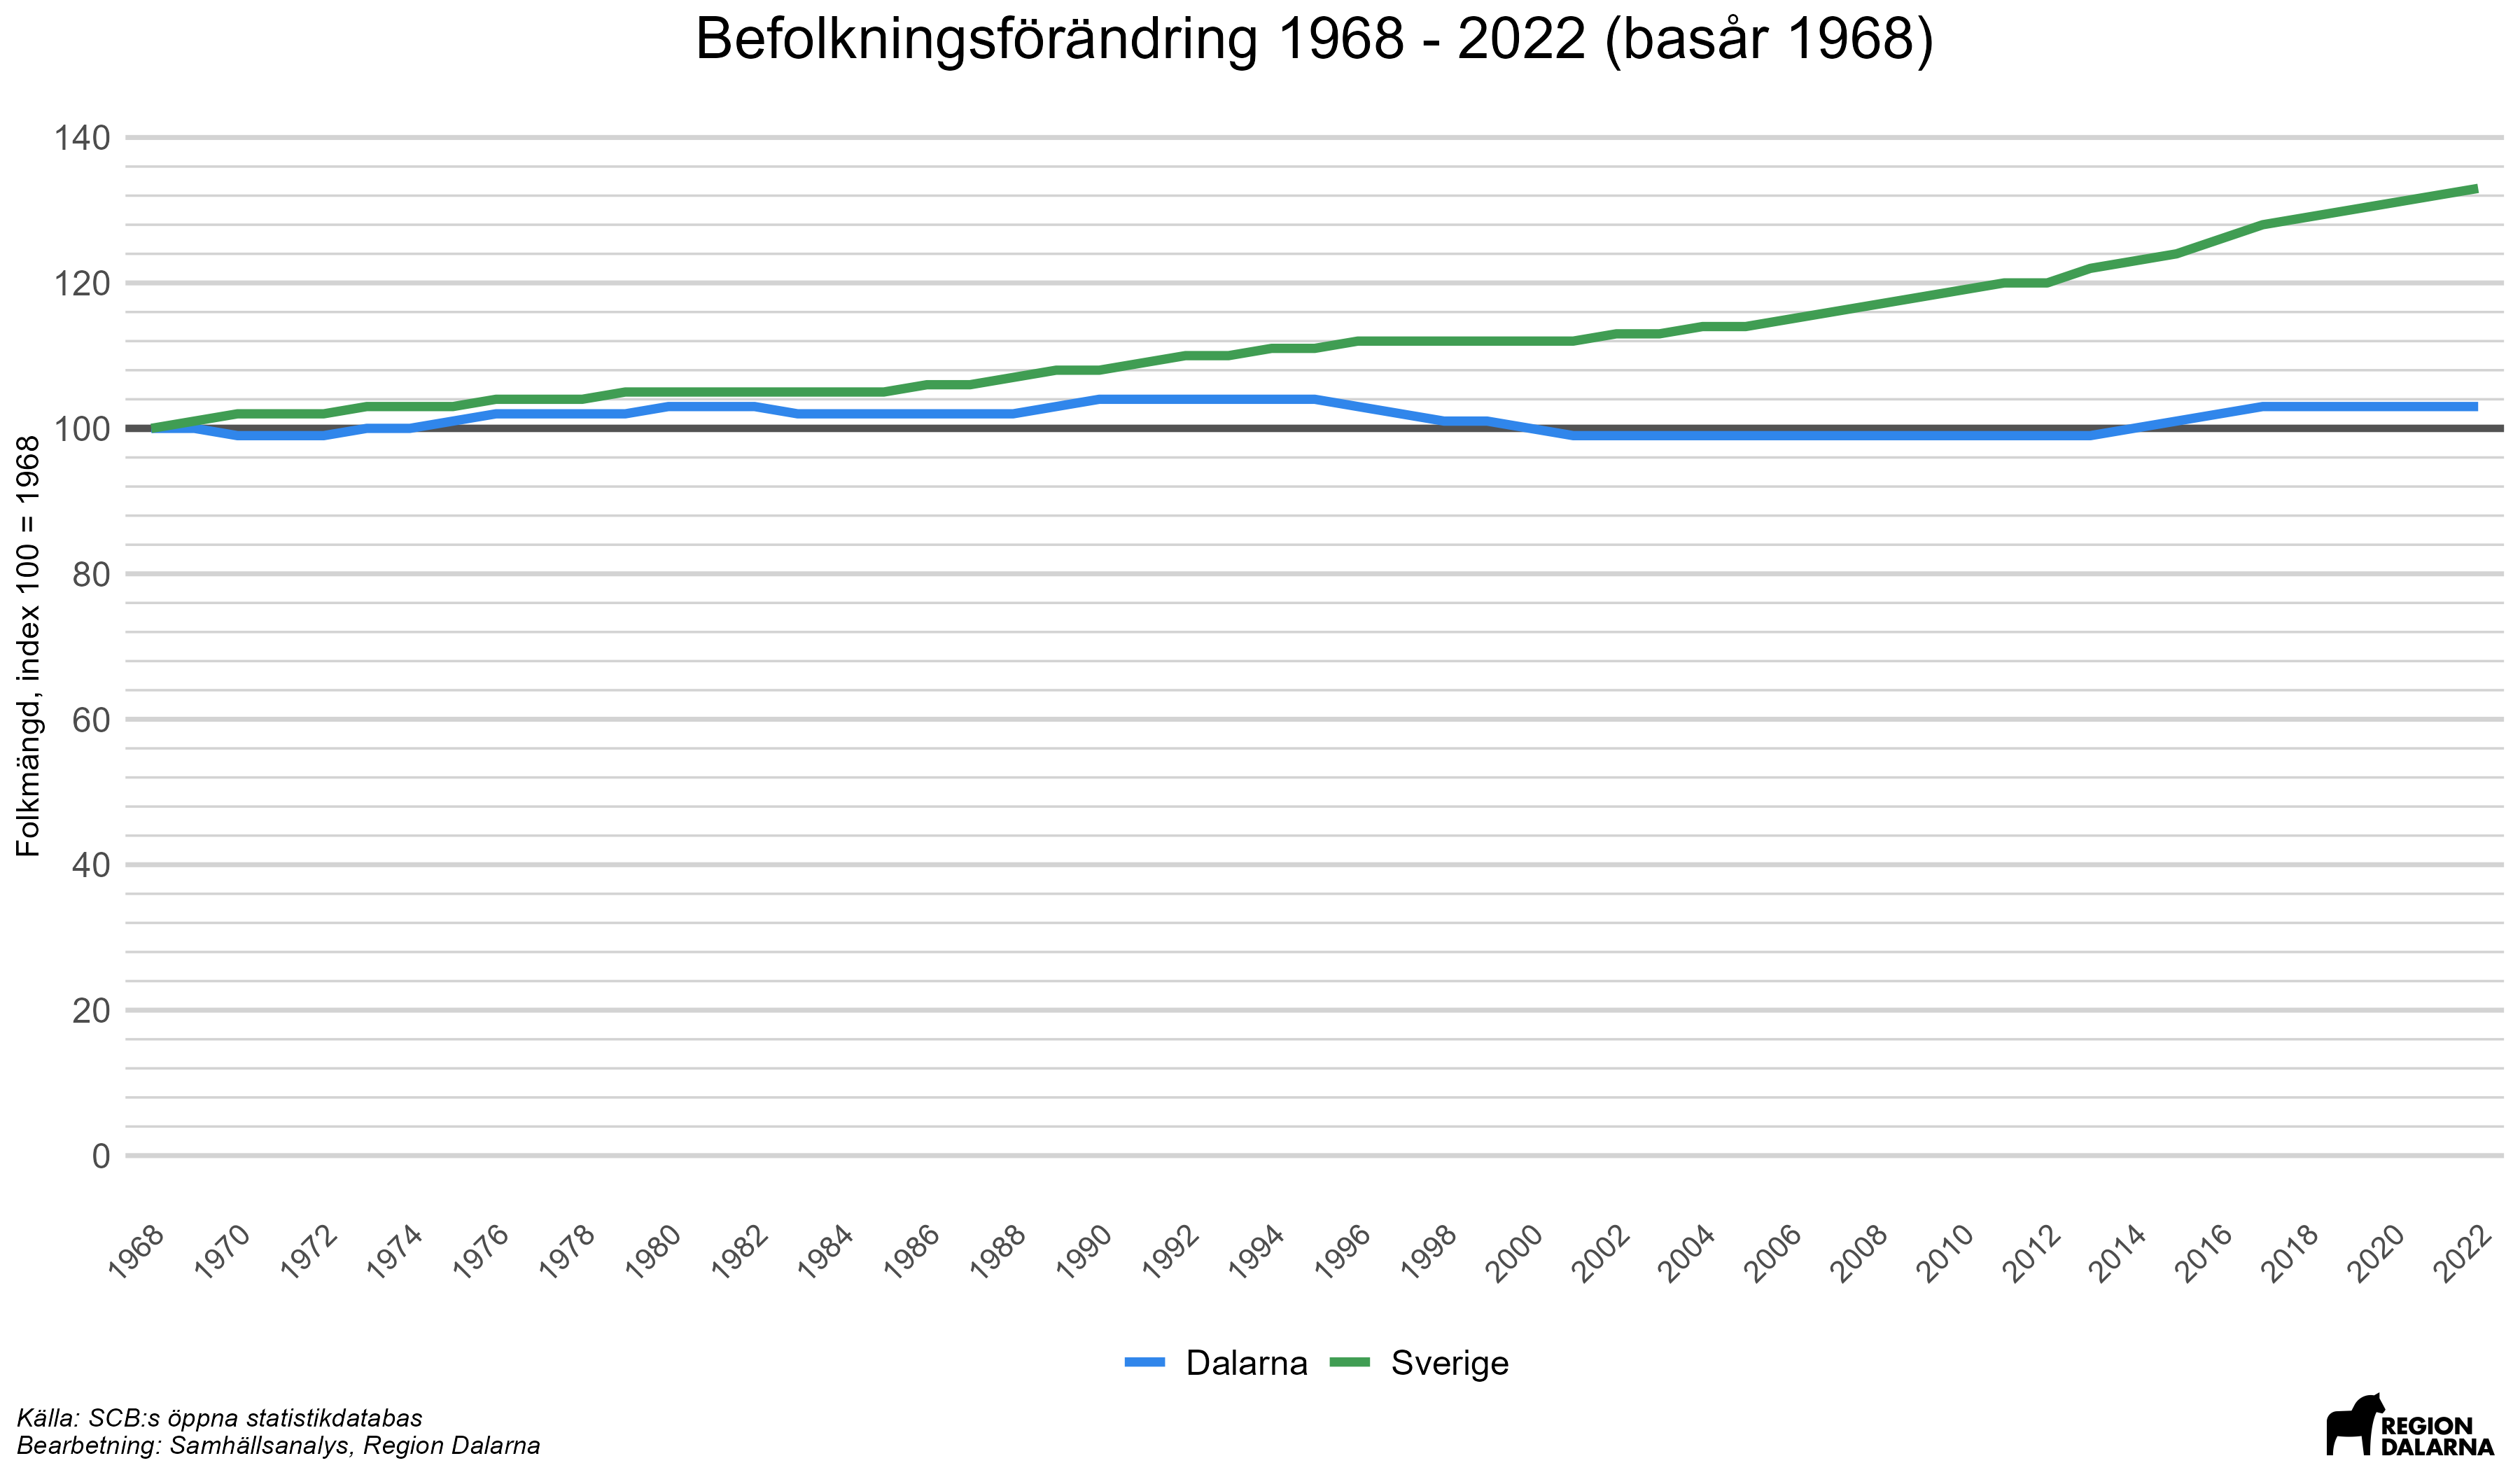
\includegraphics[width=0.9\linewidth]{G:/skript/projekt/kvinnor_man/Projekt_kvinnor_man/Diagram/befolkning_forandring} \end{center}

Befolkningen i Dalarna var 2021 relativt jämnt fördelade mellan könen,
men med något fler män än kvinnor. Åldersstrukturen har förändrats
avsevärt sedan slutet av 60-talet, vilket en jämförelse av staplarna och
de svarta linjerna i diagrammet nedanför visar. Den främsta förändringen
i länet är en förskjutning mot en allt äldre befolkning: 1968 var
relativt få personer i Dalarna 65 år eller äldre, medan åldersgrupperna
15-24 år (födda efter andra världskriget) och 45-54 (primärt födda under
mellankrigsåren) var större än idag.

Inom den äldsta ålderskategorin (85 år och äldre) finns en betydligt
större andel kvinnor än män. För yngre åldersgrupper är fördelningen
mellan män och kvinnor jämnare, men något fler män än kvinnor i
åldersgrupperna 15-24 år och 25-34 år.

\begin{center}\includegraphics[width=0.9\linewidth]{G:/skript/projekt/kvinnor_man/Projekt_kvinnor_man/Diagram/Befpyramid Dalarnas län 2021_jmfr_ar_1968} \end{center}

Dalarnas befolkning är äldre än befolkningen i de flesta andra svenska
län. I Dalarna är ungefär 23 procent av befolkningen äldre än 65 år,
vilket är tredje högst i Sverige efter Gotland och Kalmar län. Den
lägsta andelen äldre återfinns i Stockholms län där drygt 15 procent av
befolkningen är äldre än 65 år. Generellt tenderar befolkningen att vara
äldre i regioner med glesare och mindre befolkning utan större urbana
center jämfört med län där det finns större städer.

\begin{center}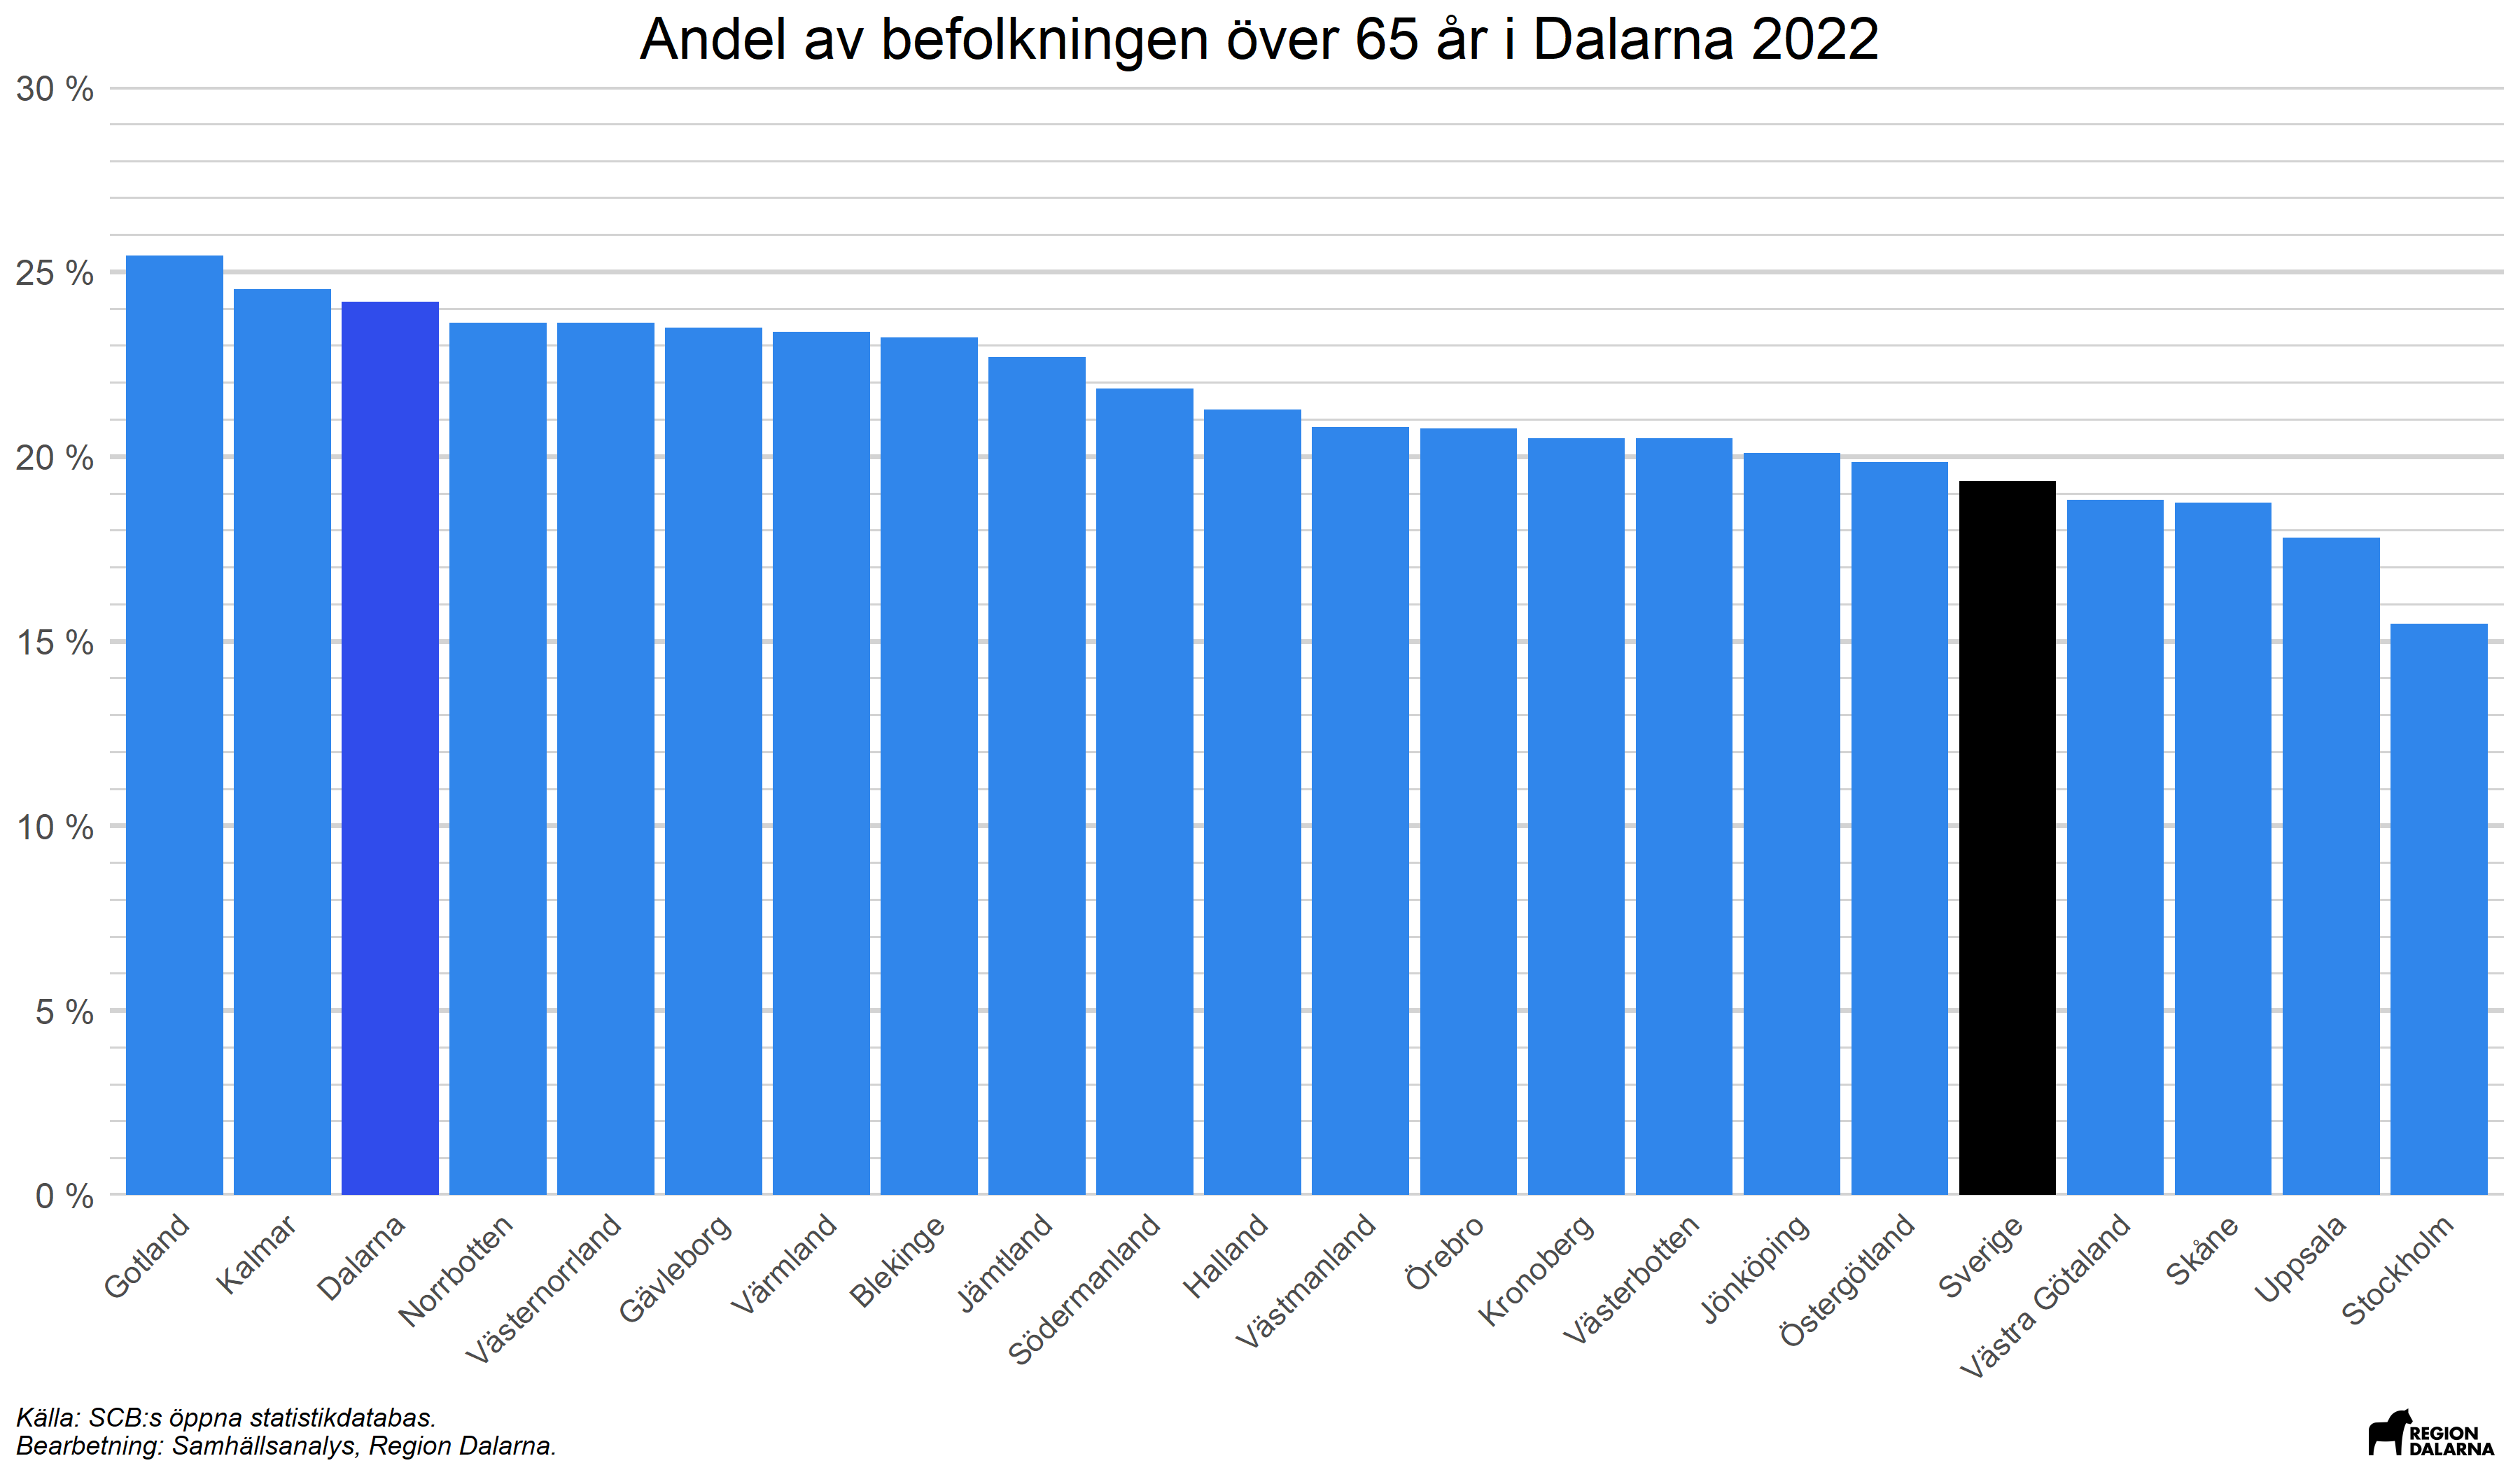
\includegraphics[width=0.9\linewidth]{G:/skript/projekt/kvinnor_man/Projekt_kvinnor_man/Diagram/andel_over_65_Sverige} \end{center}

Åldersstrukturen för inrikes och utrikes födda invånare i Dalarna
skiljer sig åt (se figuren nedan).Jämförelsevis få utrikes födda är unga
eller äldre i Dalarna, medan en betydligt större andel är i arbetsför
ålder (20-64 år) bland utrikes födda än bland inrikes födda. En
konsekvens av att inrikes födda i högre utsträckning når pensionsålder
blir att en större andel än tidigare av befolkningen i arbetsför ålder
(20-64 år) kommer att utgöras av utrikes födda.

\begin{center}\includegraphics[width=0.9\linewidth]{G:/skript/projekt/kvinnor_man/Projekt_kvinnor_man/Diagram/Befpyramid Dalarnas län 2021_jmfr_utr_inr} \end{center}

\hypertarget{utbildning-och-arbetsmarknad}{%
\section{Utbildning och
arbetsmarknad}\label{utbildning-och-arbetsmarknad}}

\hypertarget{utbildning}{%
\subsection{Utbildning}\label{utbildning}}

Utbildningsnivån för åldersgruppen 25-64 år redovisas i figuren nedan
och visar på skillnader mellan könen. Kvinnor har generellt en högre
utbildningsnivå än män i länet. Bland kvinnor i Dalarna är den
vanligaste, med 28 procent, utbildningsnivån ``eftergymnasial utbildning
som är 3 år eller längre''. Inom den här utbildningskategorin är
motsvarande siffra för män i Dalarna knappt 15 procent. I kombination
med ``kortare eftergymnasiala studier (högst 2 år)'' är det totalt 42
procent av kvinnorna i Dalarna som har någon form av eftergymnasial
utbildning. För män i länet är motsvarande siffra cirka 26 procent.

Bland män i Dalarna är den vanligast förekommande utbildningskategorin
``genomgången gymnasieutbildning på 3 år''. Drygt 30 procent av männen i
Dalarna återfinns inom denna kategori. Ytterligare drygt 26 procent av
männen har en gymnasieutbildning om högst 2 år. Sammantaget innebär
detta att drygt 56 procent av alla män i Dalarna har en
gymnasieutbildning som högsta utbildning. Motsvarande siffra för kvinnor
i Dalarna är 45 procent.

\begin{center}\includegraphics[width=0.9\linewidth]{G:/skript/projekt/kvinnor_man/Projekt_kvinnor_man/Diagram/utbildningsniva_Dalarnas län} \end{center}

I jämförelse med andra län har Dalarna relativt få personer med hög
utbildning. Andelen kvinnor med en högre utbildning om minst 3 år är 28
procent och motsvarande siffra för män i länet är cirka 14 procent.
Detta utfall placerar Dalarna som sämst i klassen, tillsammans med
Gävleborg, Kalmar och Södermanlands län som har liknande låga siffror.

Generellt tenderar regioner med större urbana center att både ha en
yngre och en mer välutbildad befolkning jämfört med mer glest befolkade
län som Dalarna. Skillnaden är störst bland män, där andelen
högutbildade män i Stockholms län är mer än dubbelt så hög som
motsvarande andel i Dalarnas län.

\begin{center}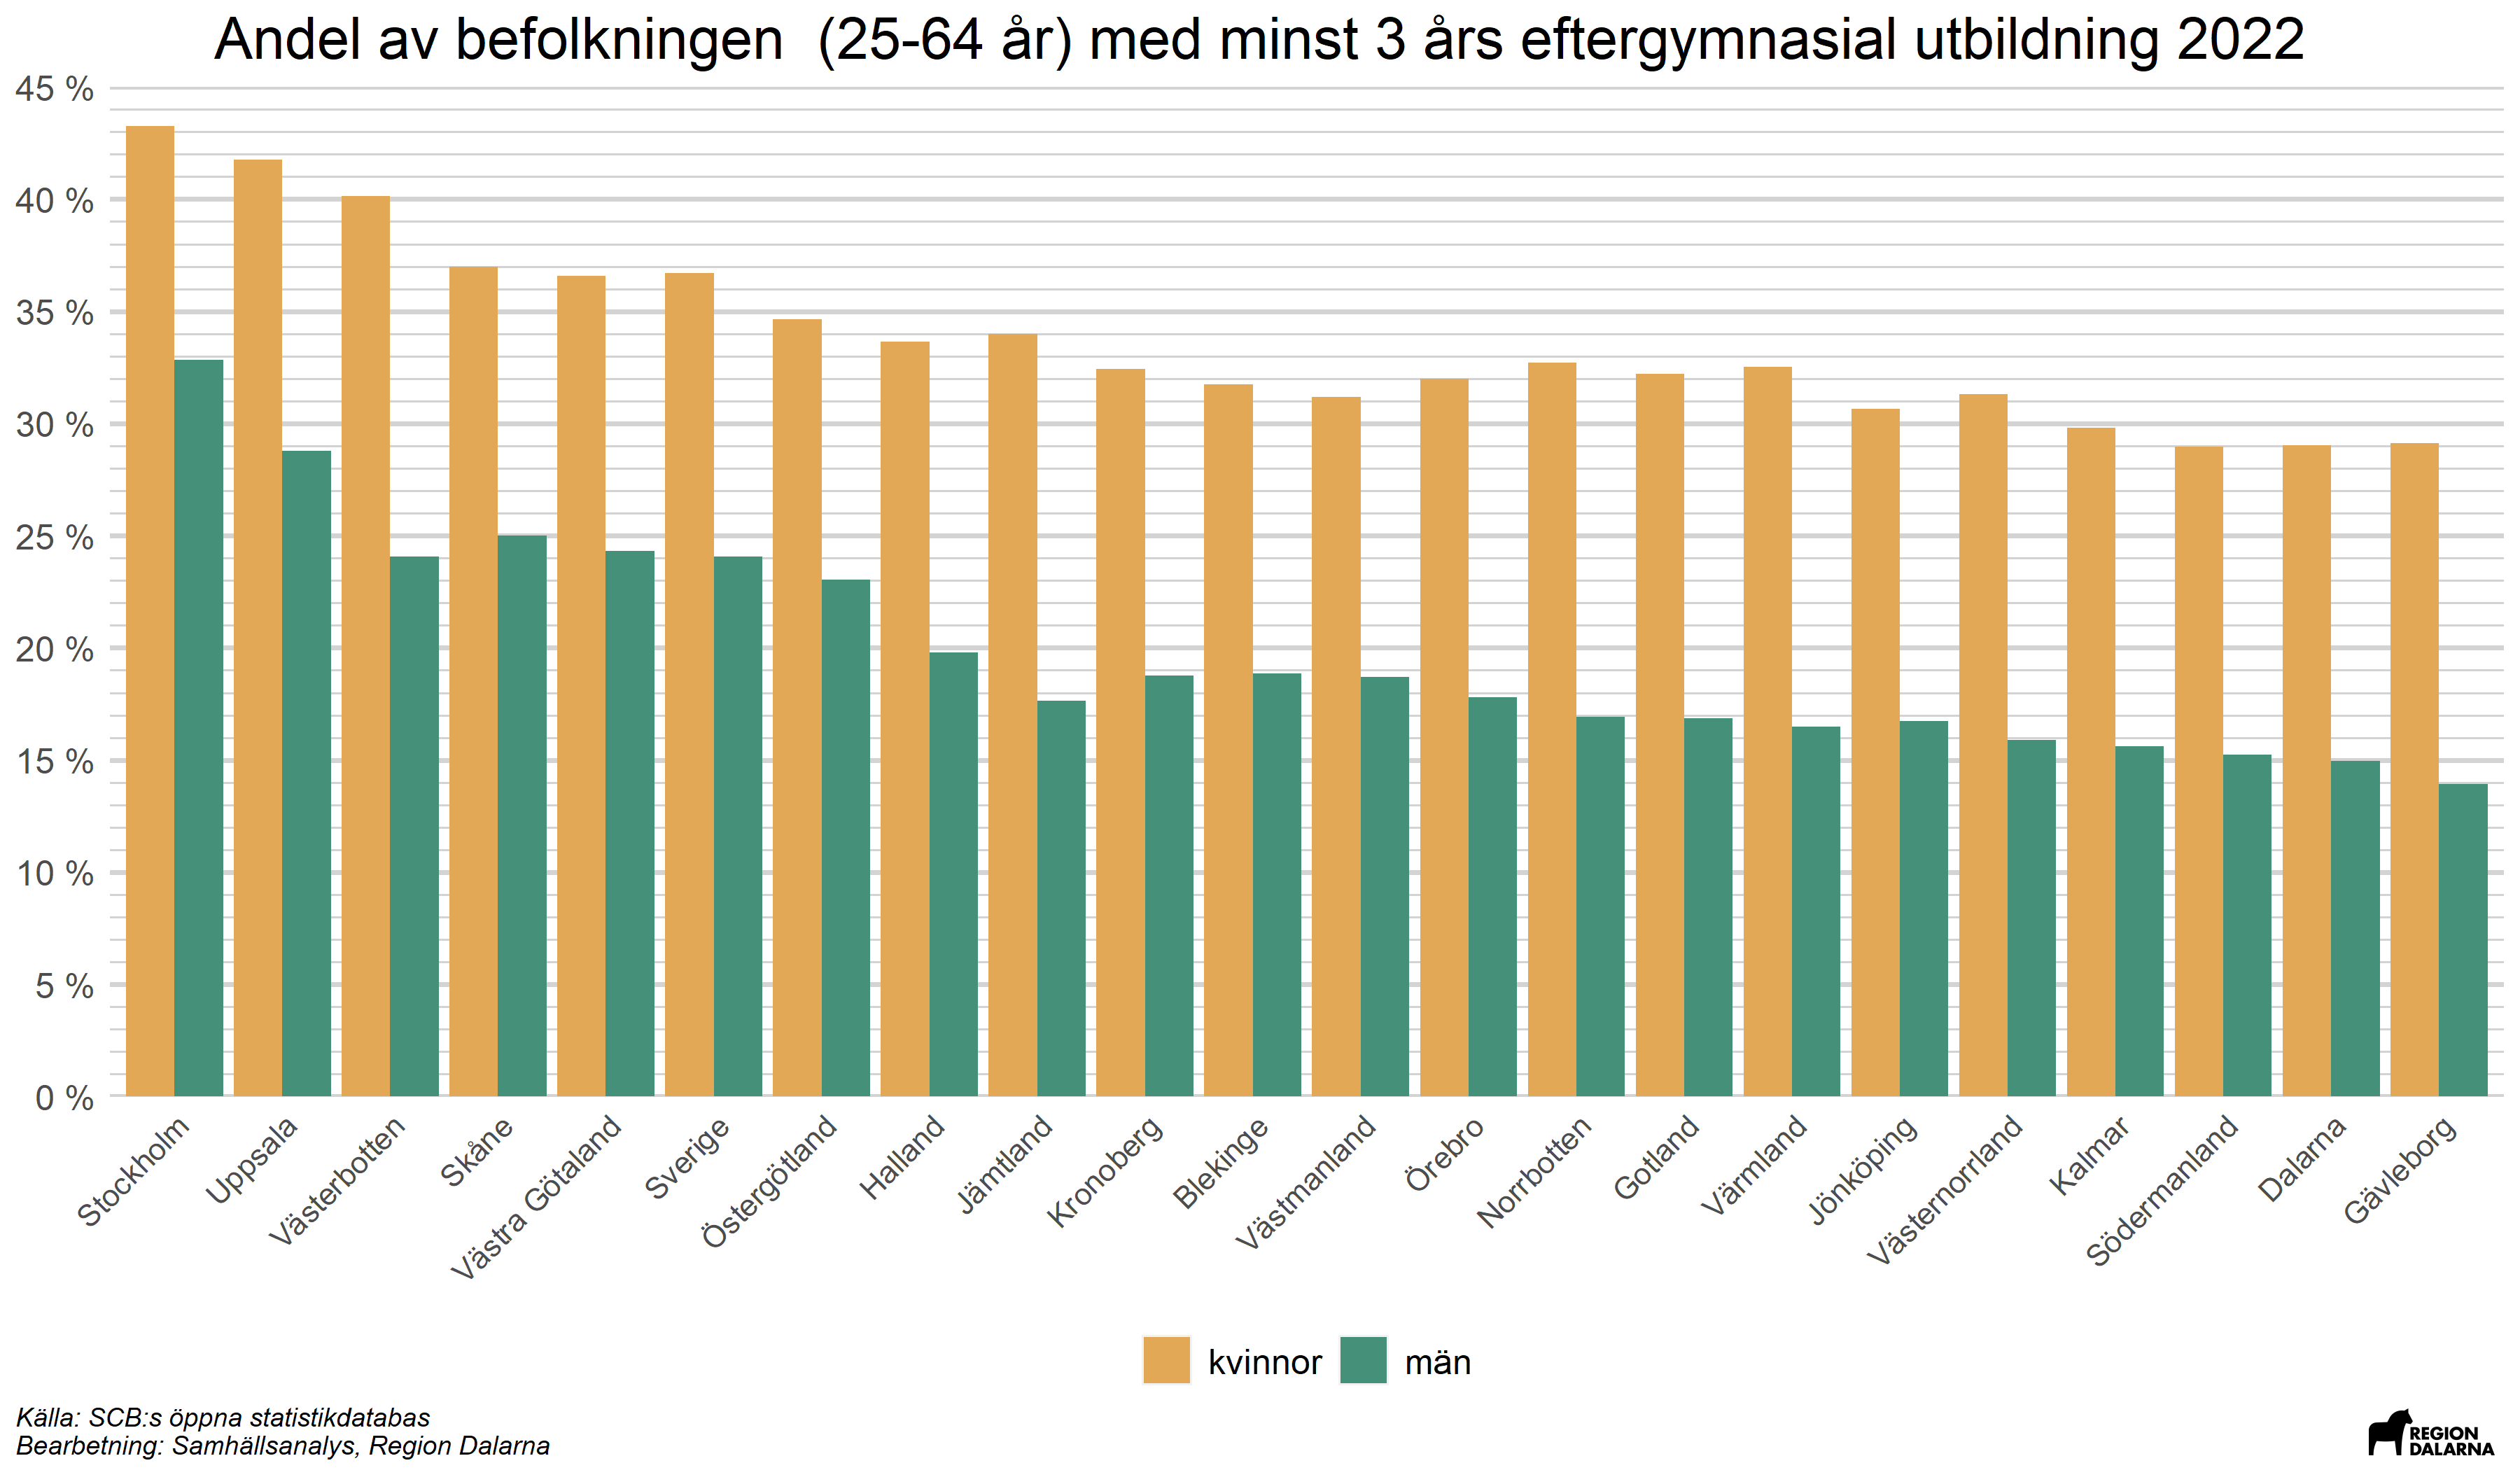
\includegraphics[width=0.9\linewidth]{G:/skript/projekt/kvinnor_man/Projekt_kvinnor_man/Diagram/utbildningsniva_jmf_lan_kon} \end{center}

Andelen av befolkningen i Dalarna med högre utbildning ökat de senaste
decennierna. Bara drygt 7 procent av befolkning hade en högre utbildning
i mitten av 80-talet. 2021 hade den andelen ökat till drygt 28 procent
för kvinnor och ungefär 15 procent för män. Anmärkningsvärt är också att
skillnaden i utbildningsnivå mellan könen har ökat avsevärt genom åren.
I mitten av 80-talet var andelen högutbildade ungefär lika stor bland
kvinnor och män. 2021 var nästan dubbelt så många kvinnor som män
högutbildade i Dalarna.

\begin{center}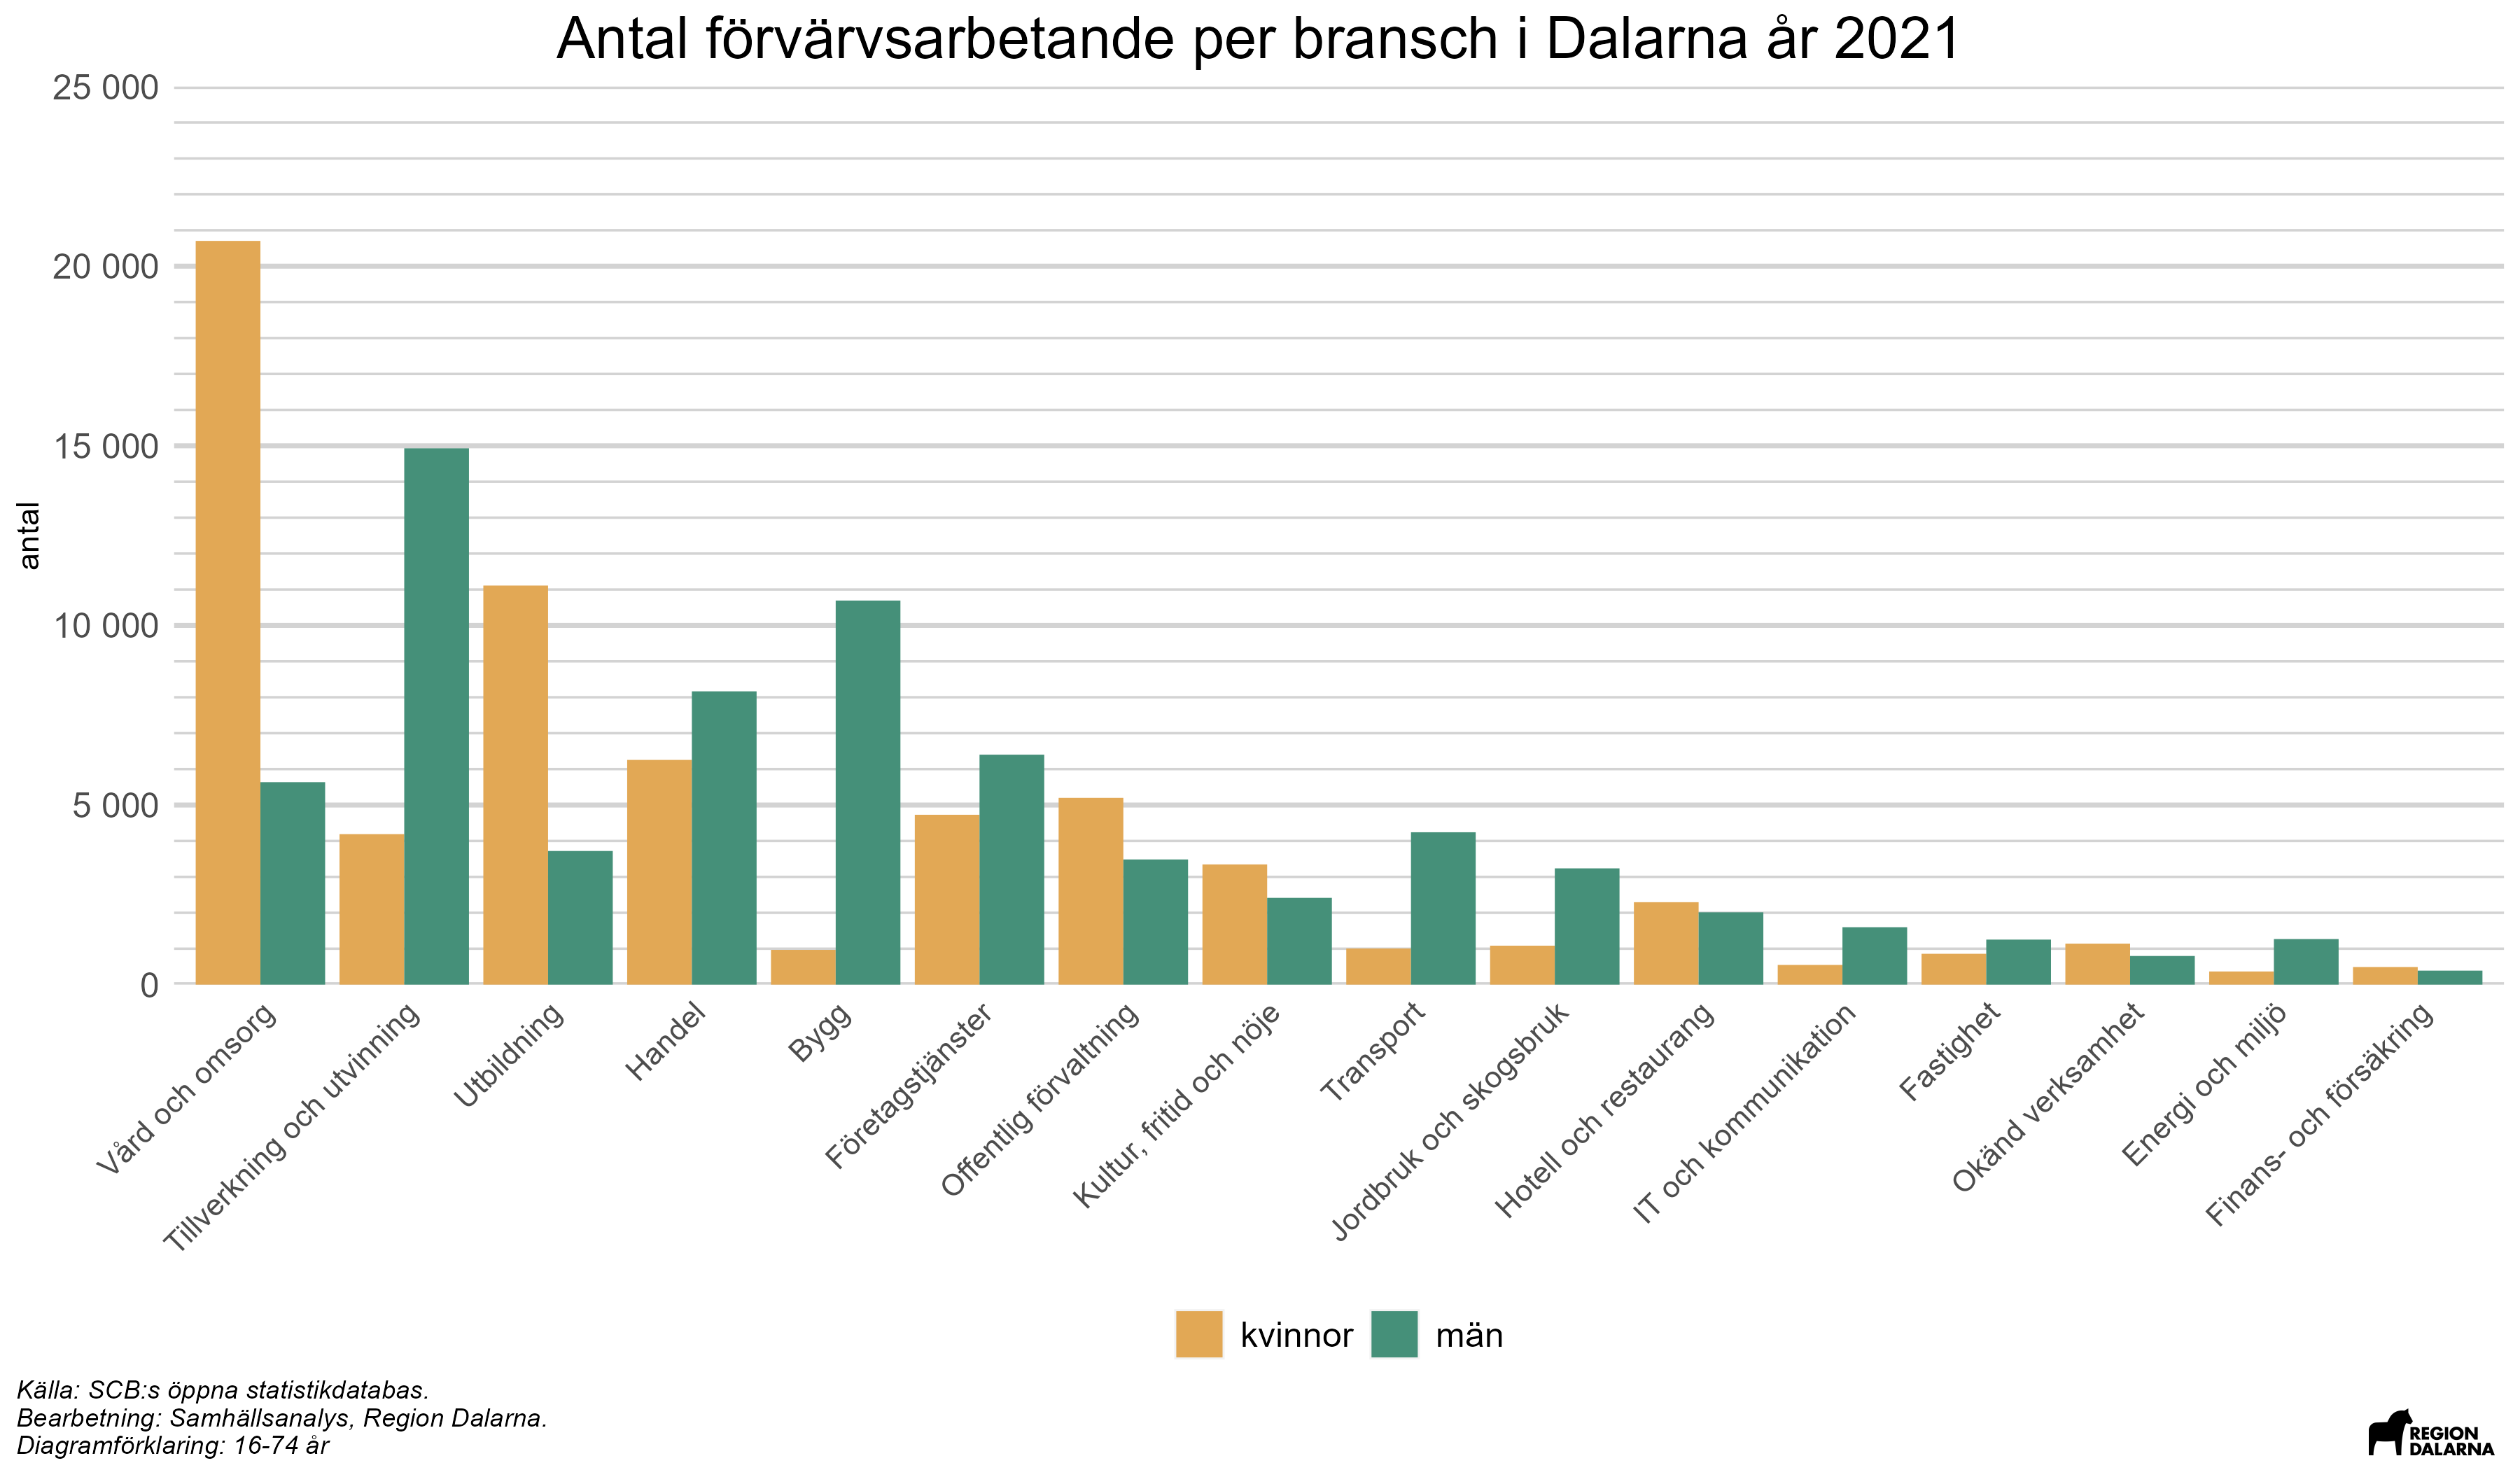
\includegraphics[width=0.9\linewidth]{G:/skript/projekt/kvinnor_man/Projekt_kvinnor_man/Diagram/utbildningsniva_85_21_kon} \end{center}

En utmaning för länet är den obalans som råder för antalet antagna till
gymnasieprogrammen i Dalarna. Av totalt 18 gymnasieprogram i länet kan
endast tre sägas vara jämställda, dvs. de har en könsfördelning där
andelen antagna är mellan 40 och 60 procent för både pojkar och flickor.
De jämställda programmen är hotell- och turismprogrammet,
introduktionsprogram, samt ekonomiprogrammet. Fem program har en
övervikt av killar, där el- och energiprogrammet har den största
obalansen följt av VVS- och fastighetsprogrammet samt bygg- och
anläggningsprogrammet. Resterande tio program har en övervikt av tjejer,
där vård- och omsorgsprogrammet är det mest obalanserade programmet
följt av hantverksprogrammet och det humanistiska programmet.

\begin{center}\includegraphics[width=1.5\linewidth]{G:/skript/jon/Presentationer/Byggforetagen juni/Indata/Konsfordelning_gymnasiet} \end{center}

\hypertarget{yrke}{%
\subsection{Yrke}\label{yrke}}

De skillnader som råder i gymnasieantagningen återspeglas i skillnader
mellan kvinnor och män senare i arbetslivet (se figuren nedan). Det
finns branscher i länet som har en tydlig övervikt av det ena eller det
andra könet, exempelvis byggbranschen, som inrymmer yrken inom bland
annat el och VVS, där män utgjorde över 90 procent av de
förvärvsarbetande 2021. Även om det har skett en ökning av andelen
kvinnor inom byggbranschen, är denna ökning försumbar. Inom vård och
omsorg är bilden den motsatta. Här utgjorde kvinnor ca 80 procent av
andelen förvärvsarbetande 2021, vilket är en något lägre andel än 2008.
Bygg samt Vård och omsorg är även de brancher som har störst övervikt
för pojkar/flickor i gymnasieantagningen, vilket innebär att en framtida
förändring i balansen mellan män och kvinnor inom olika branscher till
stor del beror på, eller kan påverkas av, en förändring i ungdomars
studieval.

Skillnader mellan kvinnor och män föreligger även på yrkesnivå. Den
största yrkesgruppen för män i Dalarnas län är kategorin som inkluderar
träarbetare och snickare, följd av yrkesförare och lagerpersonal. Dessa
yrken är typiska inom mansdominerade branscher som bygg och transport.
Bland kvinnor är det istället typiska vård och utbildningsyrken som är
vanligast. Här finns exempelvis undersköterskor, grundskollärare och
vårdbiträden. Diagrammen nedan visar de yrken i länet som flest kvinnor
respektive män utövar.

\begin{center}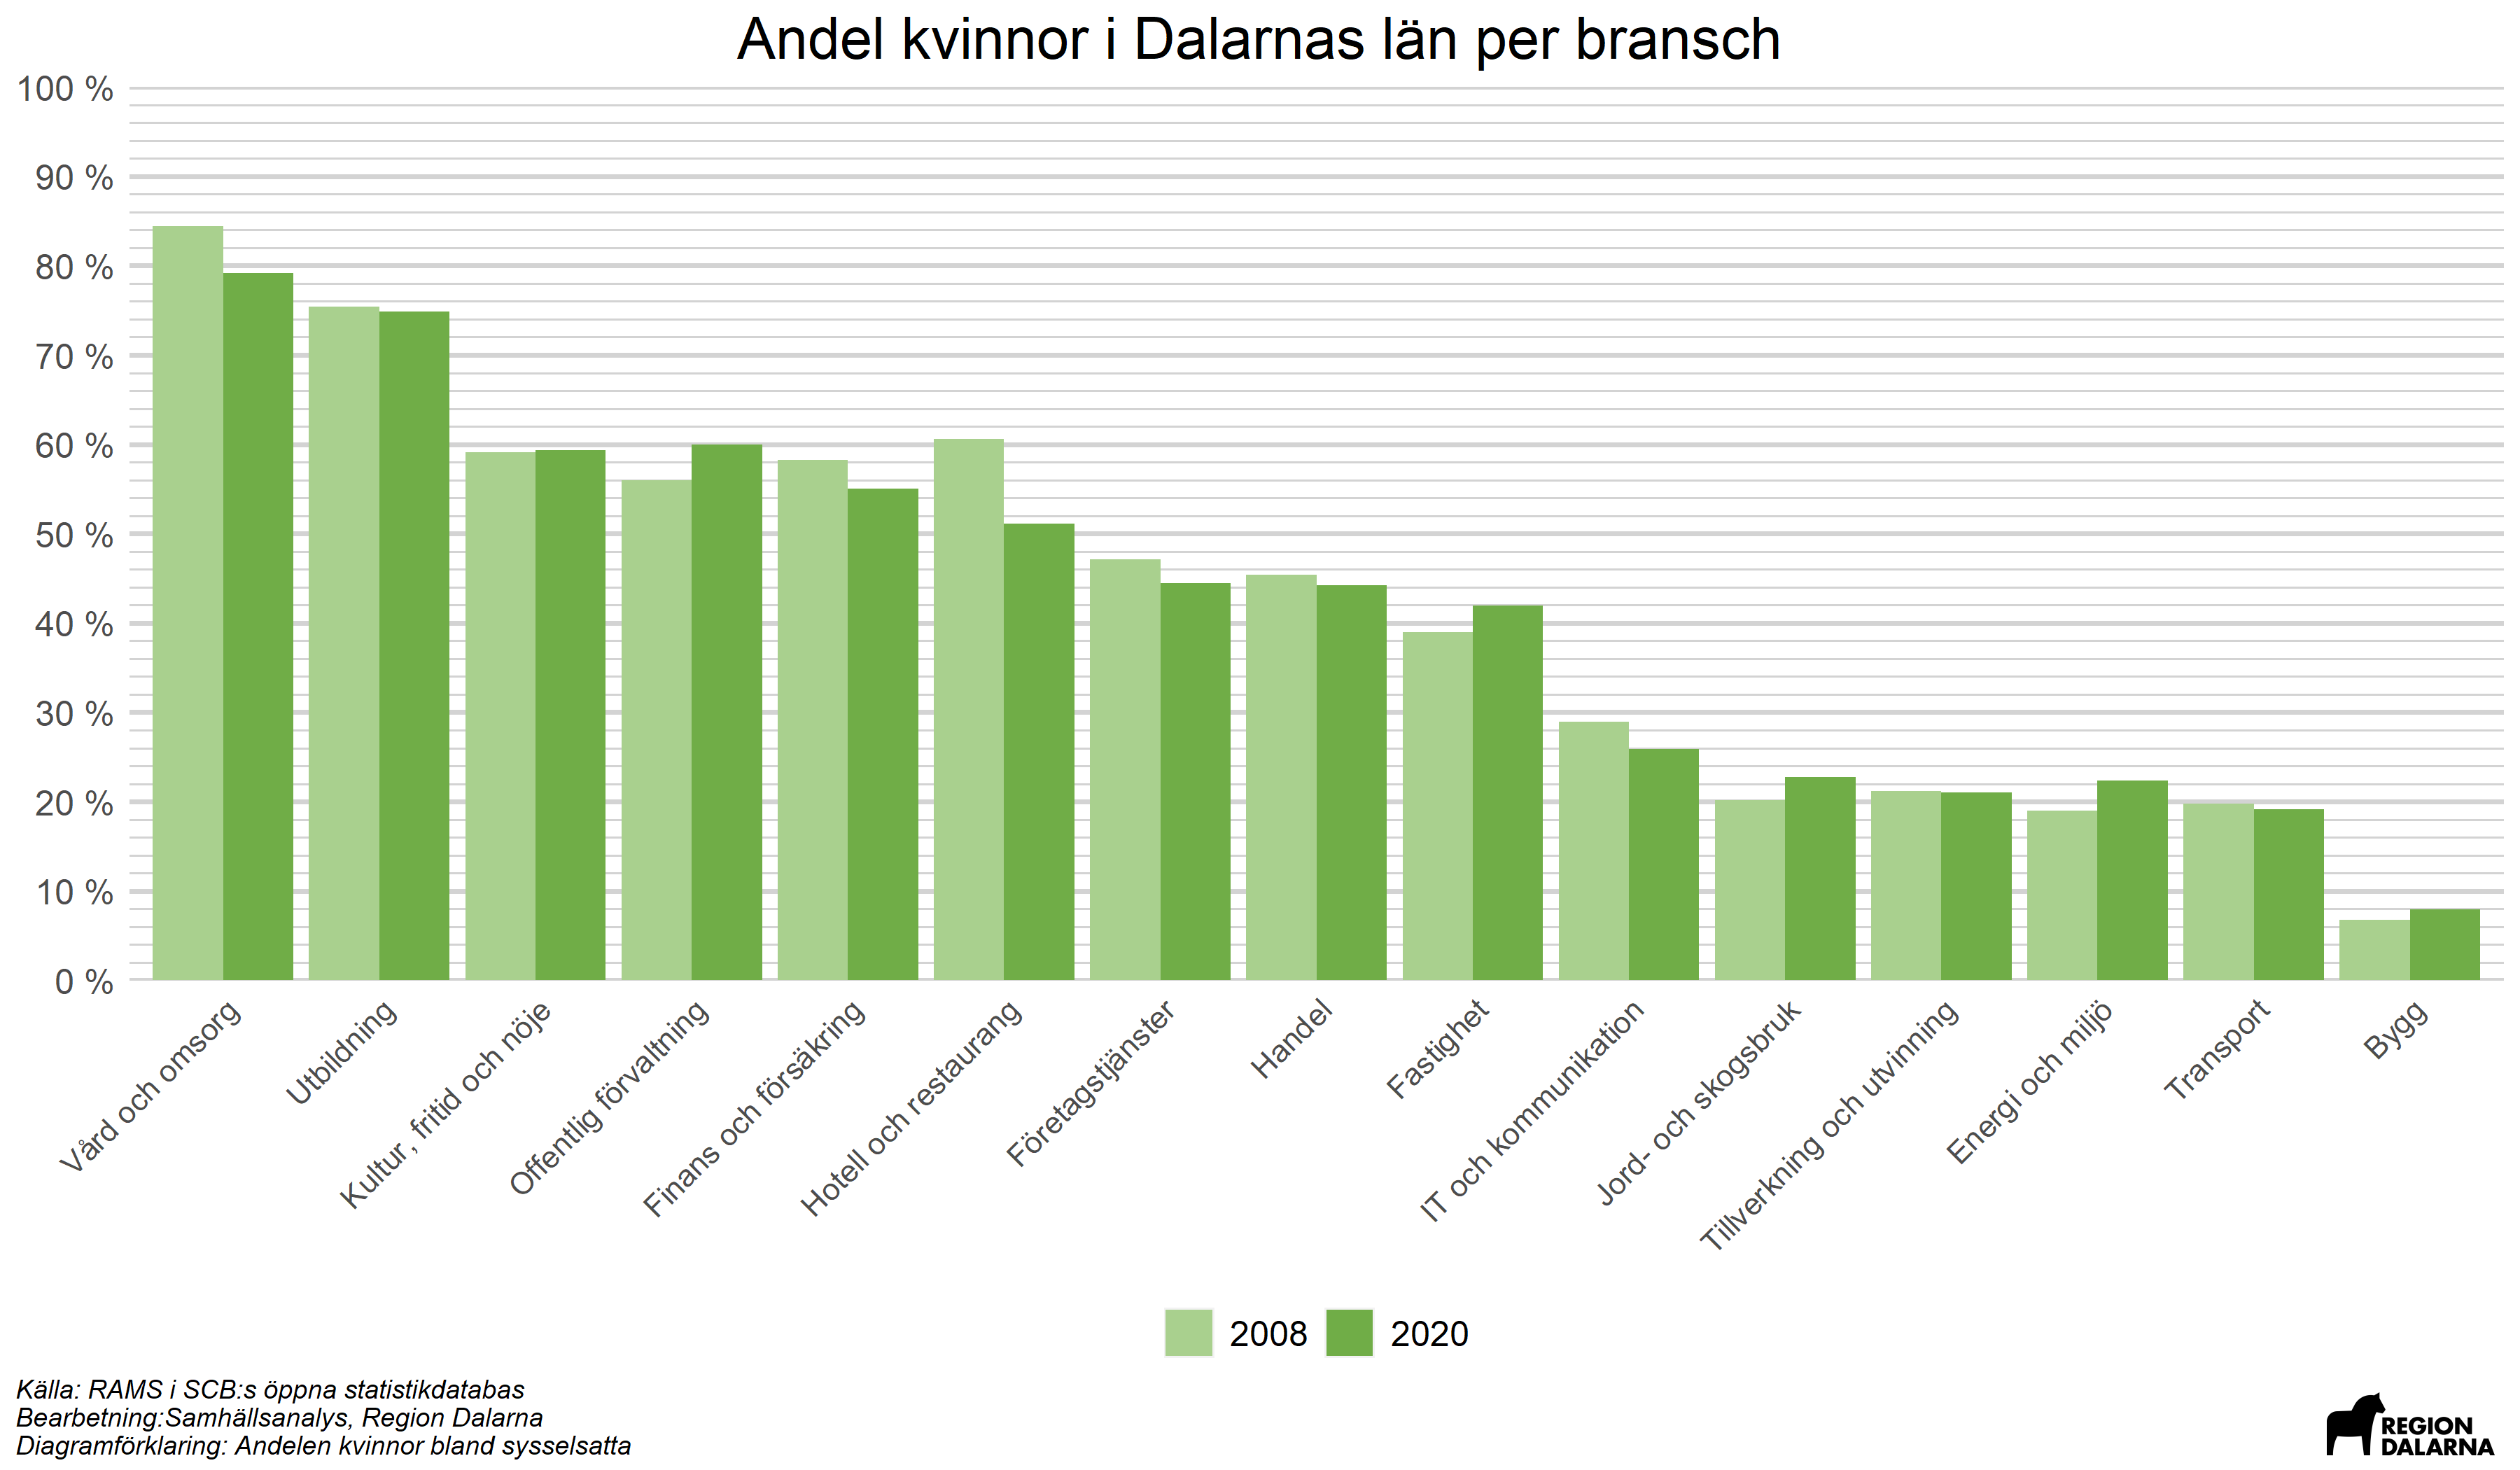
\includegraphics[width=0.9\linewidth]{G:/skript/projekt/kvinnor_man/Projekt_kvinnor_man/Diagram/Andel kvinnor i Dalarnas län per bransch_per_bransch_förändring} \end{center}

\begin{center}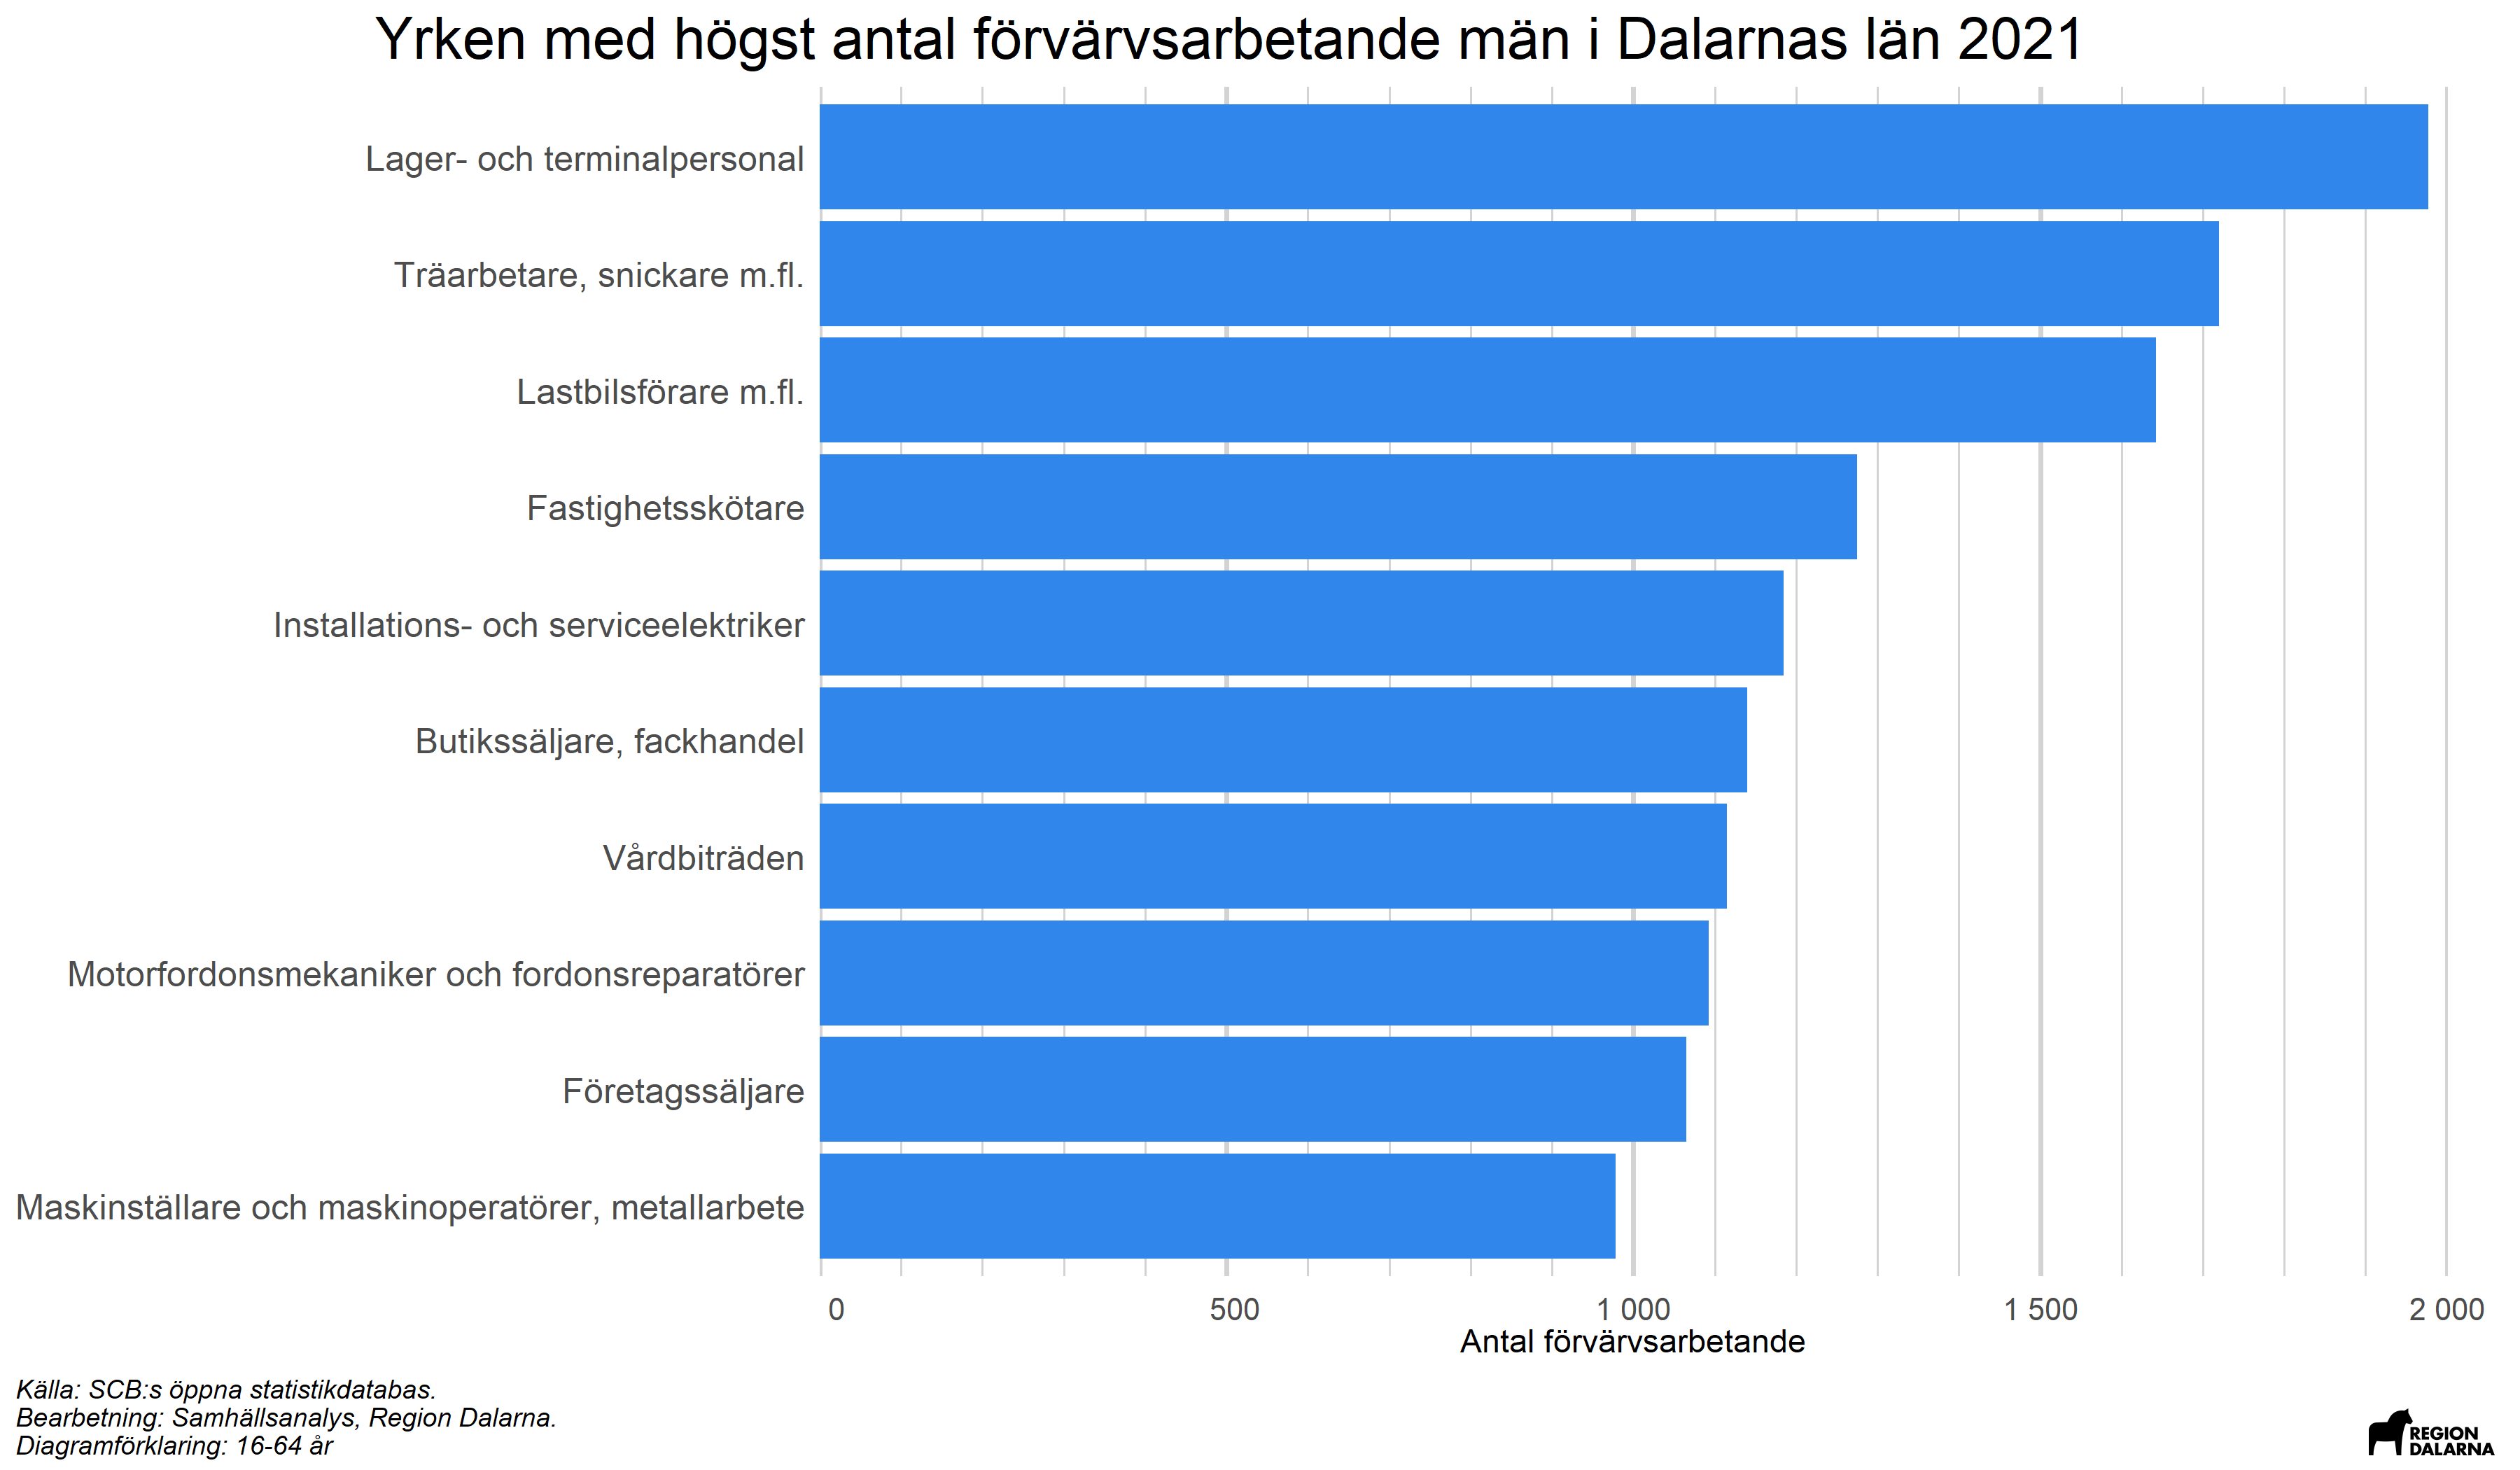
\includegraphics[width=0.9\linewidth]{G:/skript/projekt/kvinnor_man/Projekt_kvinnor_man/Diagram/yrken_man} \end{center}

\begin{center}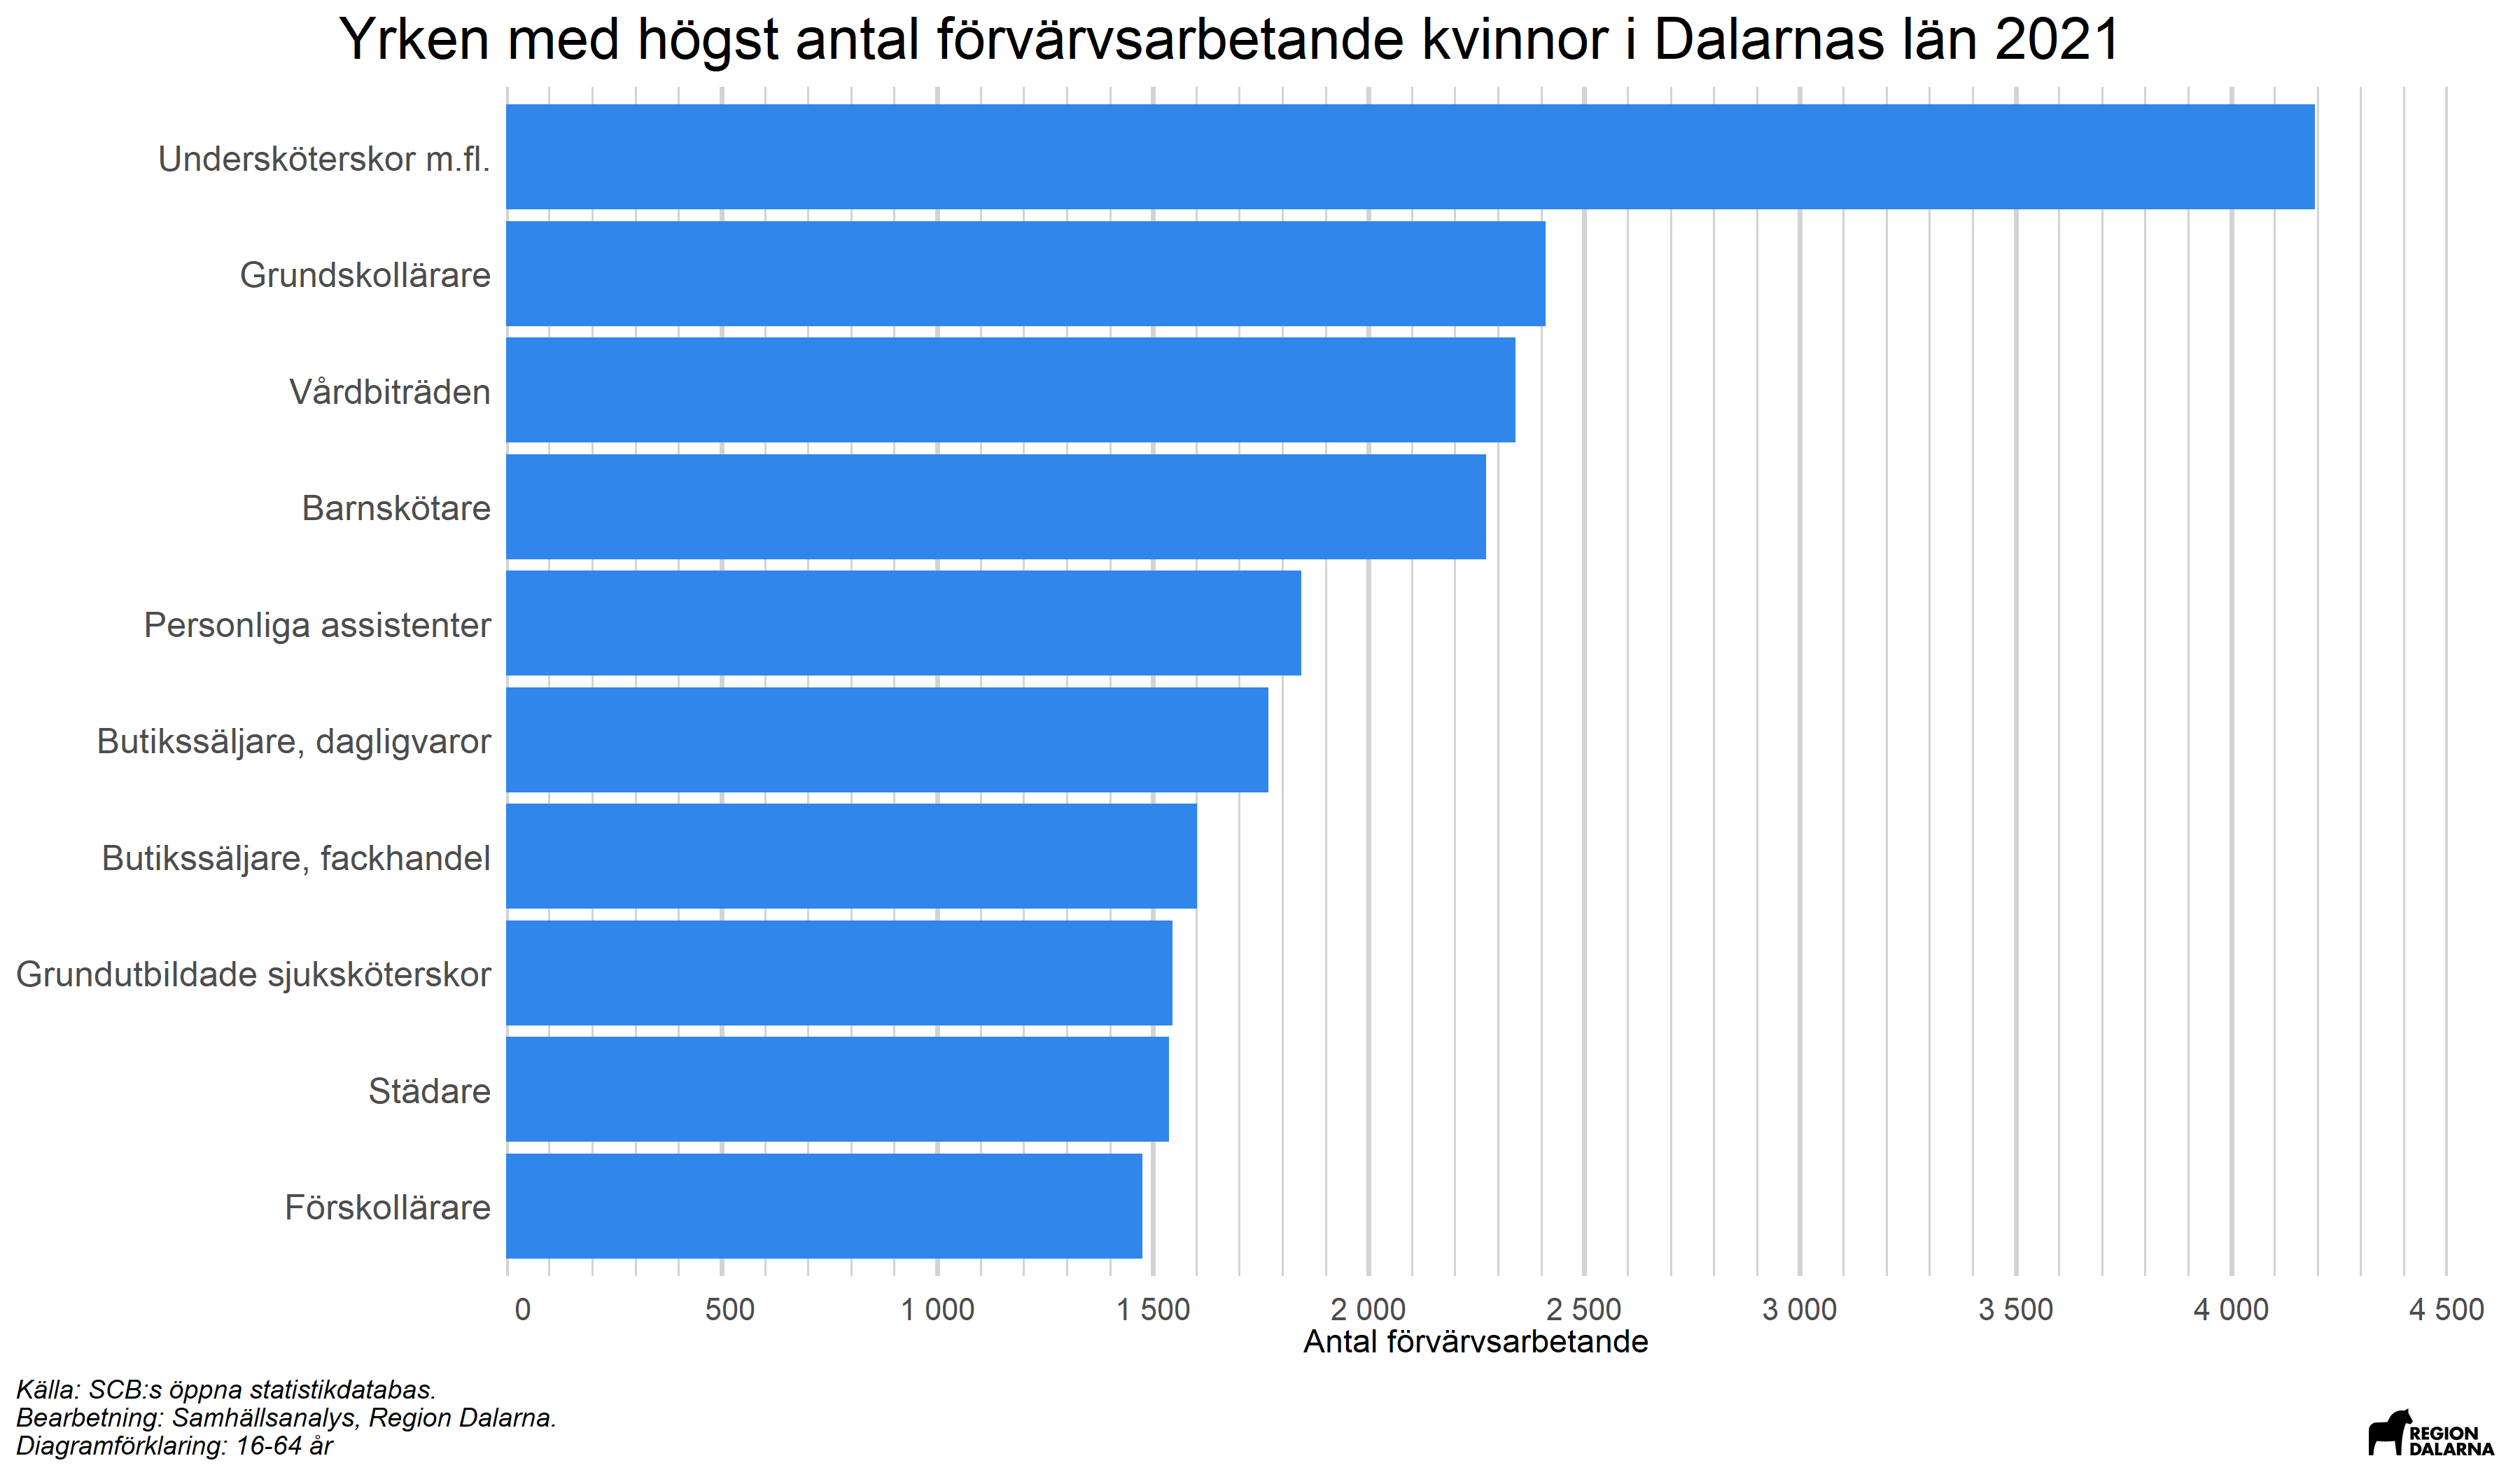
\includegraphics[width=0.9\linewidth]{G:/skript/projekt/kvinnor_man/Projekt_kvinnor_man/Diagram/yrken_kvinnor} \end{center}

\hypertarget{arbetsmarknadsstatus}{%
\subsection{Arbetsmarknadsstatus}\label{arbetsmarknadsstatus}}

Sysselsättningsgraden, det vill säga utsträckningen i vilken människor i
arbetsför ålder (20-64 år) arbetar, skiljer sig åt mellan inrikes och
utrikes födda. Sysselsättningsgraden bland utrikes födda är lägre än
sysselsättningsgraden för inrikes födda i samtliga svenska län. Det
finns även skillnader mellan kvinnor och män. För inrikes födda, det
vänstra diagrammet nedan, är sysselsättningsgraden för båda könen
ungefär lika hög. Variationen i sysselsättningsgrad mellan länen är även
den ganska liten.

För utrikes födda (det högra diagrammet nedan) är bilden annorlunda.
Utrikes födda män har en högre sysselsättningsgrad än utrikes födda
kvinnor i samtliga län förutom Norrbotten. I Dalarna är
sysselsättningsgraden bland utrikes födda män drygt 66 procent, vilket
är ungefär 8 procentenheter mer än för utrikes födda kvinnor i Dalarna.

\begin{center}\includegraphics[width=0.9\linewidth]{G:/skript/projekt/kvinnor_man/Projekt_kvinnor_man/Diagram/Sysselsättningsgrad_lan} \end{center}

Vad gäller sysselsättningsgrad uppvisar kommunerna i Dalarna ett
liknande mönster som länen på nationell nivå. Gruppen inrikes födda har
en högre sysselsättningsgrad i samtliga kommuner i Dalarna jämfört med
utrikes födda. Även här är sysselsättningsgraden för inrikes födda
kvinnor och män ungefär lika hög. För utrikes födda är det däremot stora
skillnader mellan kvinnor och män, men också mellan olika kommuner. I
linje med den nationella bilden är sysselsättningsgraden högre för
gruppen utrikes födda män än för utrikes födda kvinnor.
Sysselsättningsgraden för utrikes födda män skiljer sig dock åt mellan
kommuner där den högsta sysselsättningsgraden finns i Malung-Sälens
kommun (drygt 74 procent) och den lägsta i Smedjebacken (knappt 62
procent).

Skillnaderna mellan utrikes födda kvinnor och män är mer synlig mellan
kommuner i Dalarna än när länen som helhet jämförs. Gagnefs kommun har
den högsta sysselsättningsgraden för gruppen utrikes födda kvinnor, 70
procent, och ligger klart över genomsnittet för Dalarnas län (knappt 58
procent). Samtidigt är sysselsättningsgraden i Ludvika kommun bland
utrikes födda kvinnor bara drygt 50 procent. Ludvika, tillsammans med
Vansbro, har de största skillnadera i sysselsättningsgrad, ungefär 15
procentenheter vardera, mellan utrikes födda kvinnor och män.

\begin{center}\includegraphics[width=0.9\linewidth]{G:/skript/projekt/kvinnor_man/Projekt_kvinnor_man/Diagram/Sysselsättningsgrad_kommun} \end{center}

Bilden av arbetsmarknaden kompletteras genom att titta på
arbetslösheten, som visar hur många av de aktivt arbetssökande som inte
har ett jobb.En jämförelse av arbetslösheten för utrikes födda och
inrikes födda åskådligör ett antal viktiga skillnader.

Arbetslösheten är generellt mycket högre för utrikes födda än för
inrikes födda. Bland inrikes födda är arbetslösheten låg och ligger
kring 3-4 procent för kvinnor och ungefär 4-5 procent för män (se
diagrammet nedan). Arbetslösheten för inrikes födda i Dalarna ligger
något högre än rikets som helhet, men kan fortfarande beskrivas som låg.
Arbetslösheten bland utrikes födda är däremot betydligt högre i samtliga
av Sveriges län. I Dalarna är skillnaden i arbetslöshet mellan utrikes
och inrikes födda ca 18 procentenheter för kvinnor och ca 13
procentenheter för män.

Gruppen utrikes födda kvinnor har en klart högre arbetslösheten än
gruppen utrikes födda män i de flesta av Sveriges län. Ett undantag är
Norrbottens län, där arbetslösheten för utrikes födda män bara är
marginellt högre än arbetslösheten för utrikes födda kvinnor.

I figuren nedan framgår också att det finns avsevärda skillnader mellan
länen. Norrbottens har den lägsta arbetslösheten för utrikes födda med
ungefär 10-11 procent för både kvinnor och män, medan arbetslösheten
överstiger 20 procent för båda könen i såväl Gävleborg som Södermanland.
Dalarnas län ligger något över riksgenomsnittet, men uppvisar inte
extrema arbetslöshetssiffror åt något håll.

\begin{center}\includegraphics[width=0.9\linewidth]{G:/skript/projekt/kvinnor_man/Projekt_kvinnor_man/Diagram/Arbetslöshet_lan} \end{center}

Precis som var fallet med sysselsättninggrad tidigare, så uppvisar
Dalarnas kommuner ett liknande mönster som länen på nationell nivå.
Bland inrikes födda är arbetslösheten låg och något fler män än kvinnor
är arbetslösa. Högst arbetslöshet bland inrikes födda finns i Ludvika,
men skillnaden gentemot genomsnittet i länet är relativt liten. Lägst
arbetslöshet återfinns i Malung-Sälens kommun.

För utrikes födda är arbetslösheten avsevärt mycket högre för både
kvinnor och män. Genomsnittet i Dalarnas län ligger på drygt 21 procent
för utrikes födda kvinnor och drygt 18 procent för utrikes födda män. De
högsta arbetslösheterna för utrikes födda kvinnor återfinns i Avesta och
Ludvika där de ligger på över 30 procent. Avesta redovisar även den
högsta arbetslöshetssiffran för utrikes födda män med drygt 24 procent.
Lägst arbetslöshet återfinns även här i Malung-Sälens kommun.

\begin{center}\includegraphics[width=0.9\linewidth]{G:/skript/projekt/kvinnor_man/Projekt_kvinnor_man/Diagram/Arbetslöshet_kommun} \end{center}

Arbetslösheten i Dalarna för inrikes och utrikes födda visar på
skillnader över tid. För gruppen inrikes födda syns en nedgång i andelen
arbetslösa från 2010 och framåt, med ett litet avbrott i trendlinjen
under pandemiåren 2020-2021. Gruppen utrikes födda har två trendlinjer i
diagrammet nedan. Från 2006 till 2017 ökade arbetslösheten bland utrikes
födda till relativt höga nivåer jämfört med början på tidsperioden.
Arbetslösheten bland utrikes födda män i Dalarna var också konsekvent
högre än för utrikes födda kvinnor och betydligt högre under
flyktingkrisen och åren som följde. Efter flyktingkrisen, från 2017 och
framåt, har arbetslösheten bland gruppen utrikes födda minskat från
toppnivåerna och utrikes födda kvinnor har idag en något högre
arbetslöshet än utrikes födda män.

\begin{center}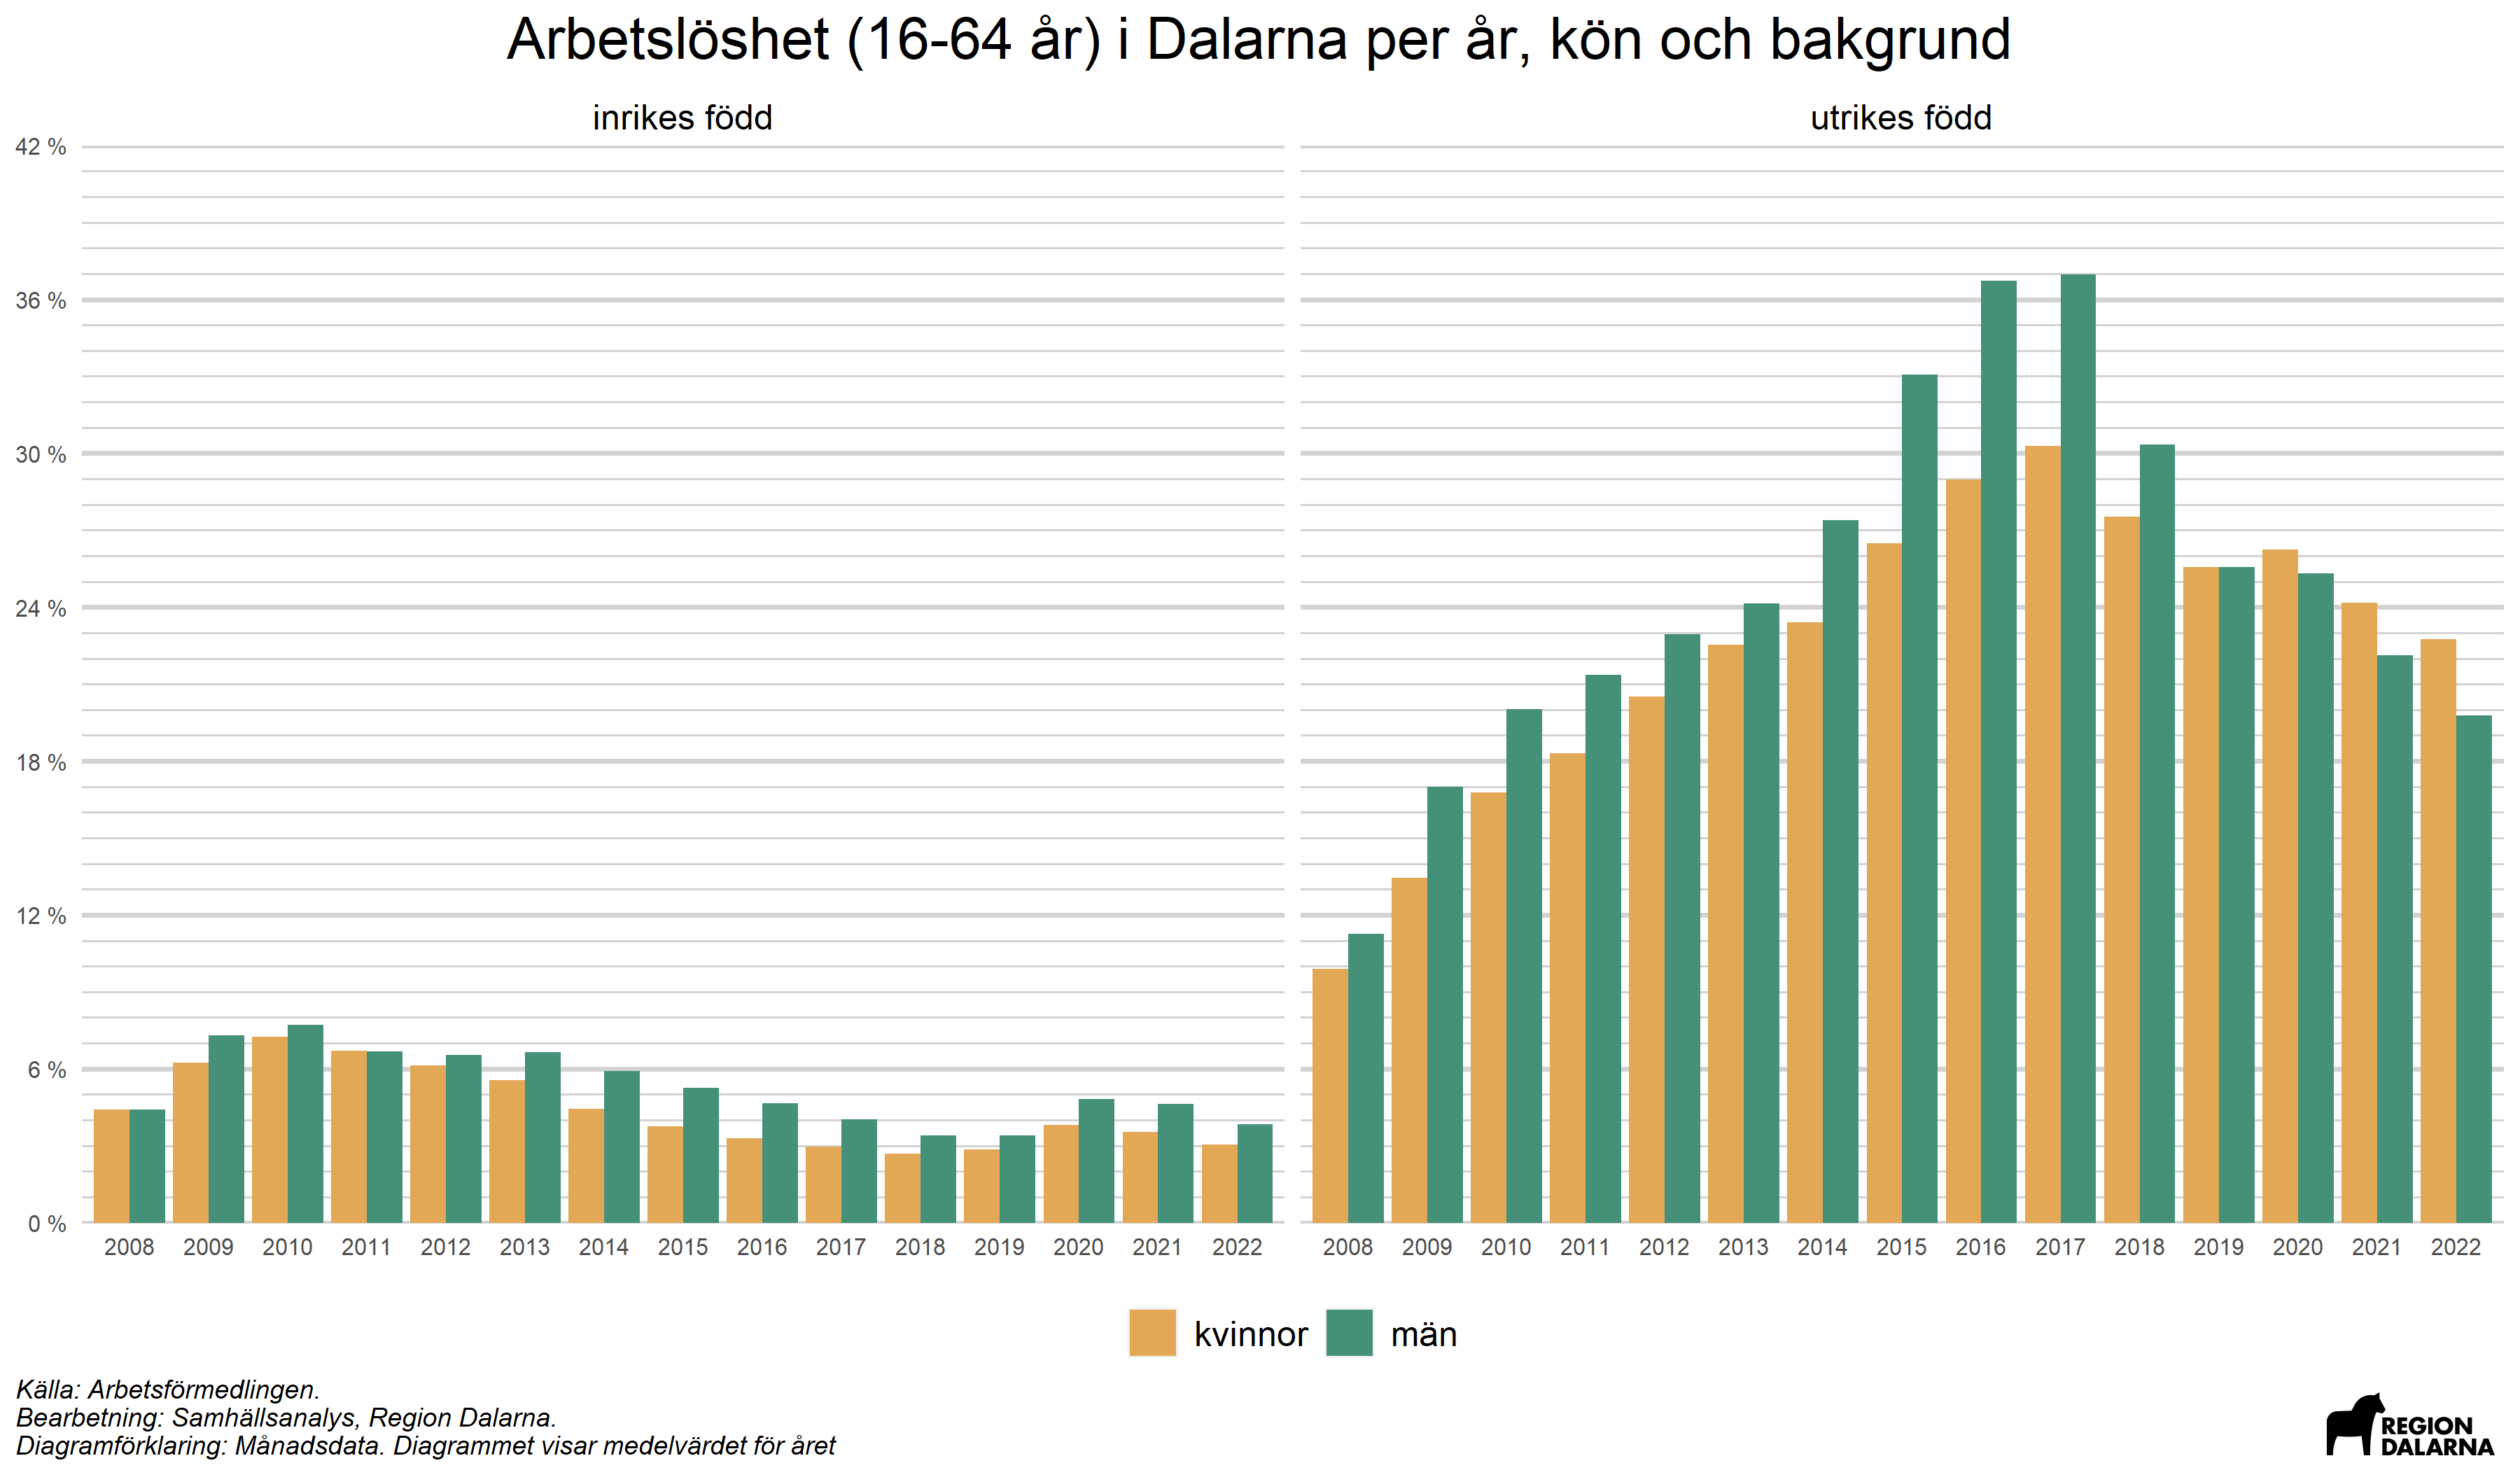
\includegraphics[width=0.9\linewidth]{G:/skript/projekt/kvinnor_man/Projekt_kvinnor_man/Diagram/arbetsloshet_Dalarna_tidsserie_bakgrund} \end{center}

Hur långt ifrån arbetsmarknaden som en individ befinner sig beror delvis
på hur länge personen har varit utan anställning. En person som har
varit arbetslös länge har ofta svårare att ta sig tillbaka in på
arbetsmarknaden. I diagrammet nedan har arbetslösa delats in i tre olika
grupper efter arbetslöshetsstid (1-12 månader, 12-24 månader samt 24+
månader). I Dalarnas län är den största gruppen arbetslösa de som inte
haft en anställning under de senaste 12 månaderna. Ungefär 2 procent av
arbetskraften har varit arbetslösa i över 24 månader och står därmed
långt från arbetsmarknaden.

\begin{center}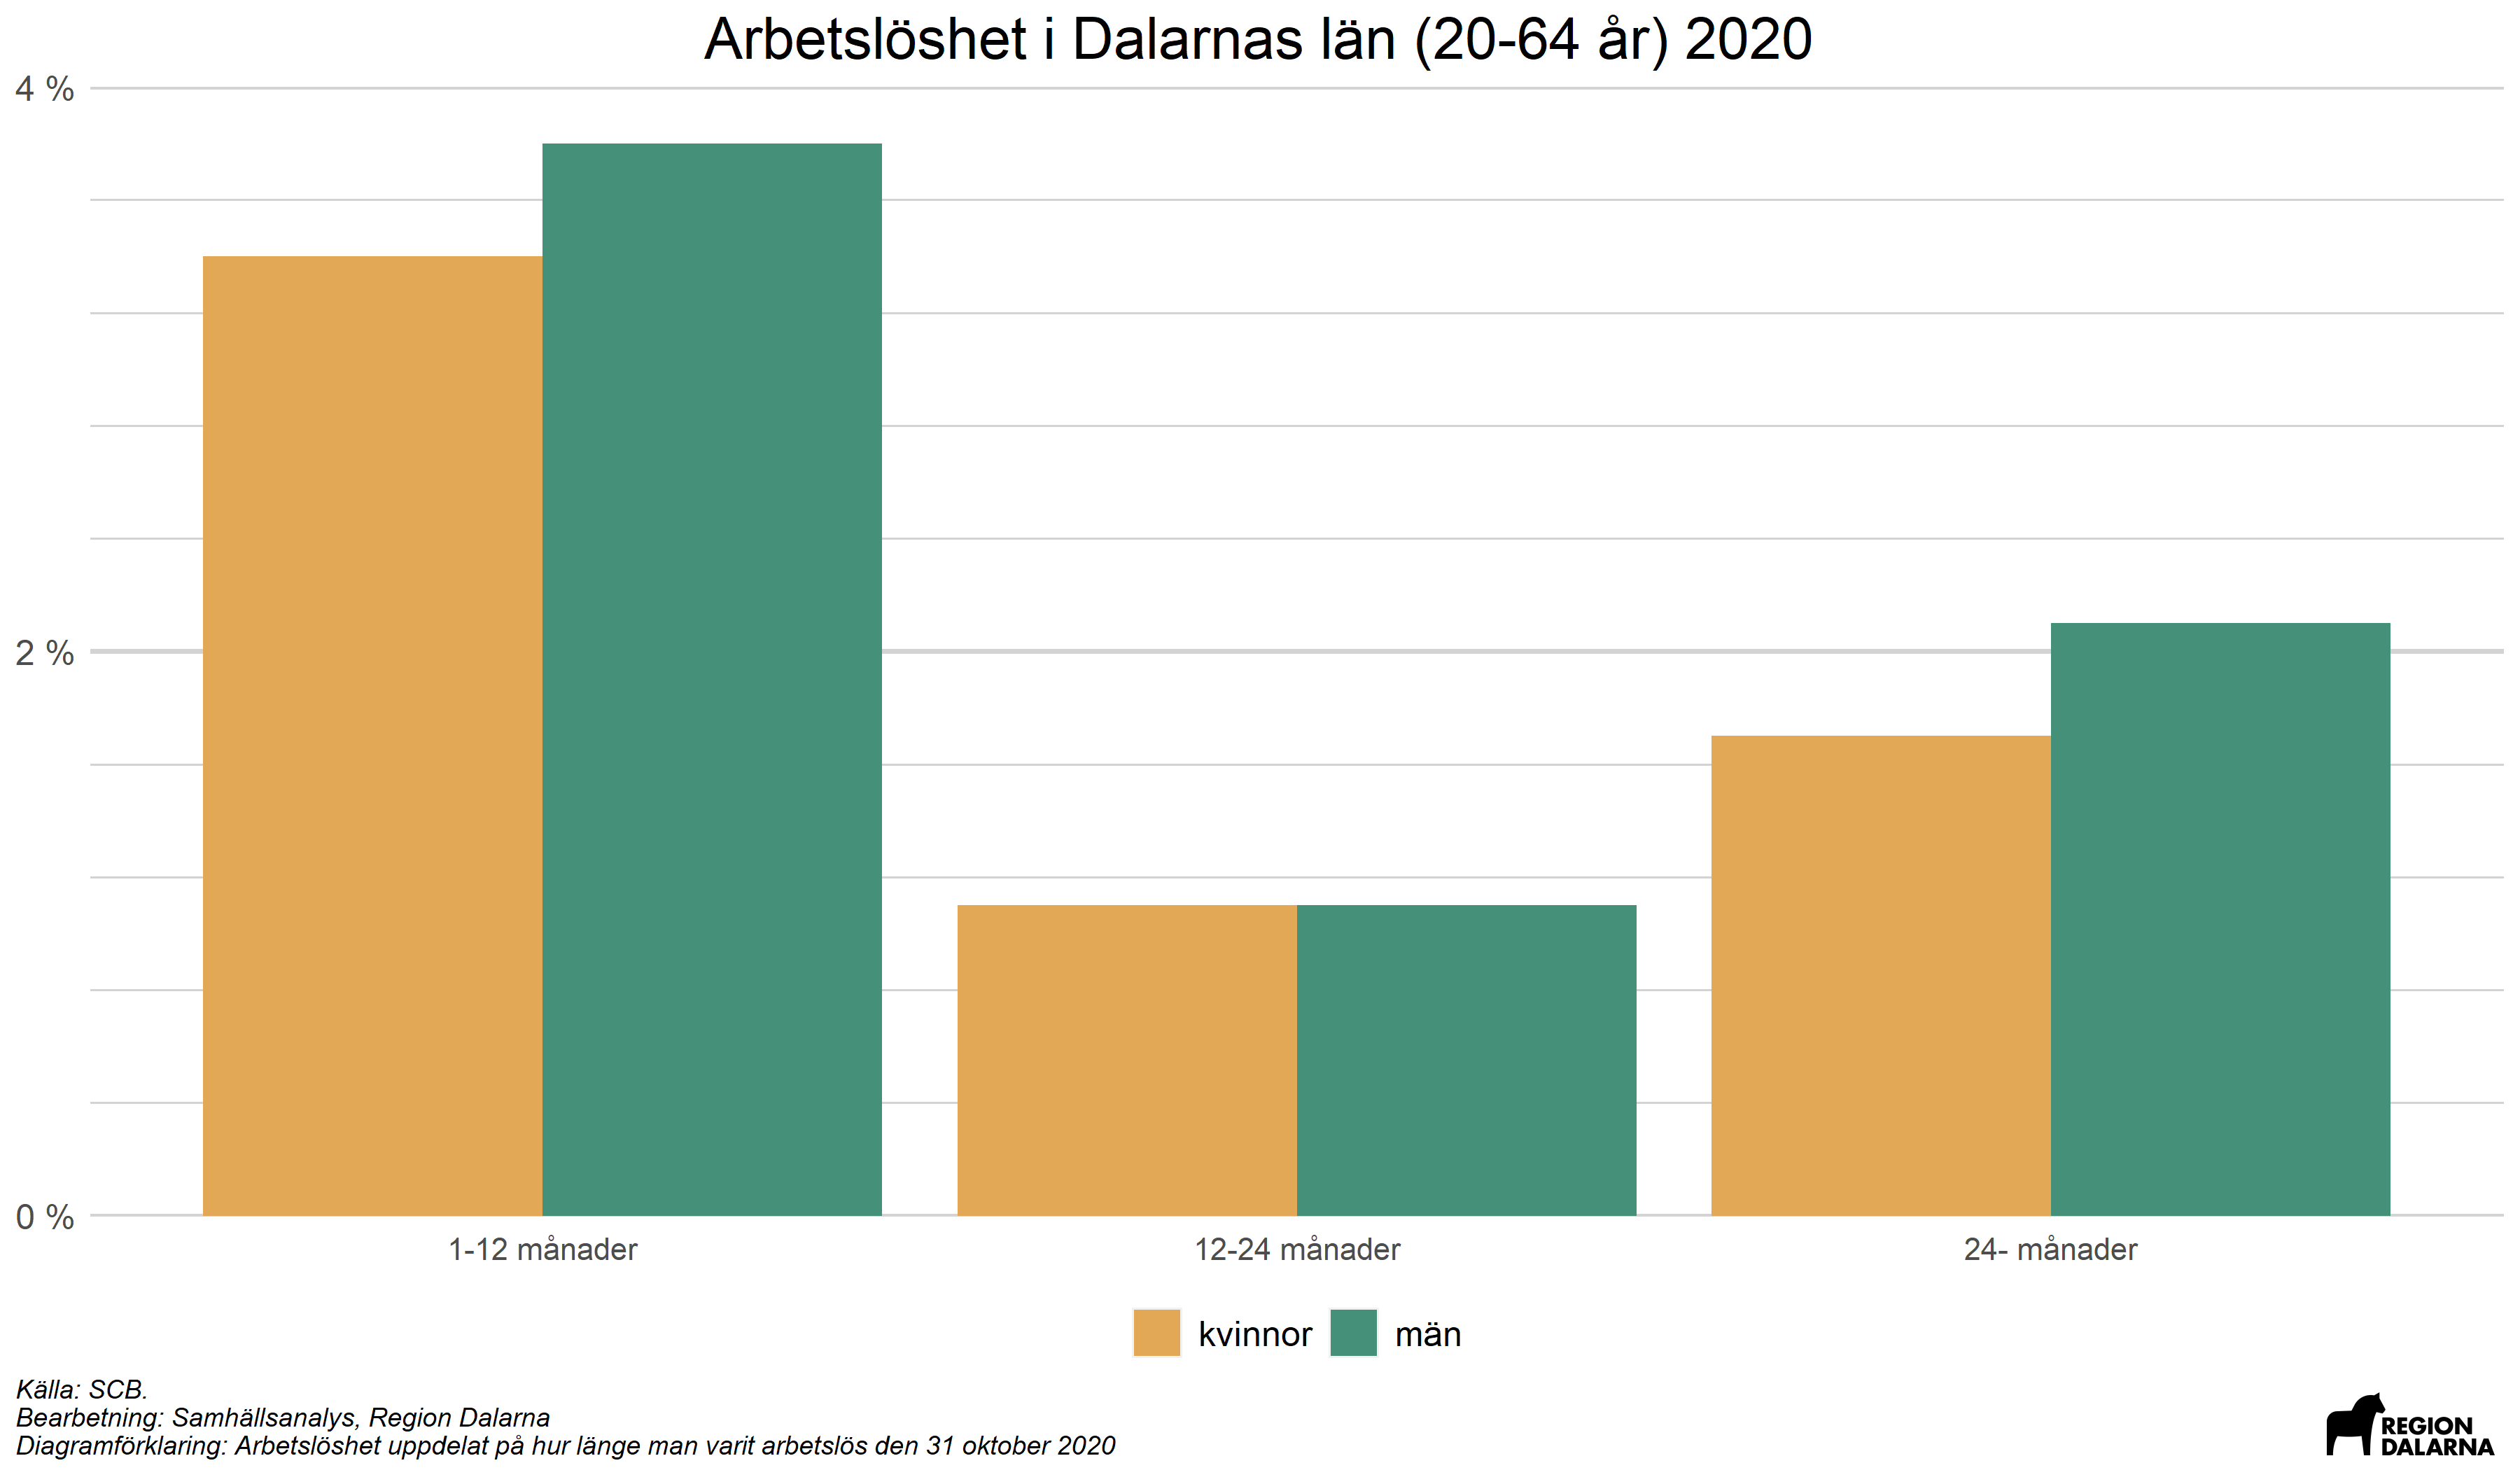
\includegraphics[width=0.9\linewidth]{G:/skript/projekt/kvinnor_man/Projekt_kvinnor_man/Diagram/langtidsarbetsloshet_lan_kon} \end{center}

\uline{\emph{OBS! DEN SUMMERADE ARBETSLÖSHETEN PÅ OLIKA LÄNGDER VERKAR
INTE ÖVERENSTÄMMA MED DEN TOTALA ARBETSLÖSHETEN HÖGRE UPP.}}

Arbetslöshetstiden skiljer sig åt mellan inrikes och utrikes födda (se
diagrammet nedan). Inrikes födda har en klart större andel arbetslösa
med kort arbetslöshetstid (\textless12 månader) än arbetslösa med lång
långtidsarbetslöshet (\textgreater12 månader). Bland utrikes födda är
bilden annorlunda. Här är gruppen långtidsarbetslösa ungefär lika stor
som andelen korttidsarbetslösa. Det är också värt att notera att en
relativt stor andel av de utrikes födda varit arbetslösa under en mycket
lång period (\textgreater24 månader).

Arbetslöshetstiden skiljer sig även mellan kvinnor och män. Bland
inrikes födda har männen en något högre grad av arbetslöshet oavsett
arbetslöshetstid. Bland utrikes födda har kvinnor en högre grad av
korttidsarbetslöshet, medan männen i större utsträckning blir fast i
längre perioder av arbetslöshet.

\begin{center}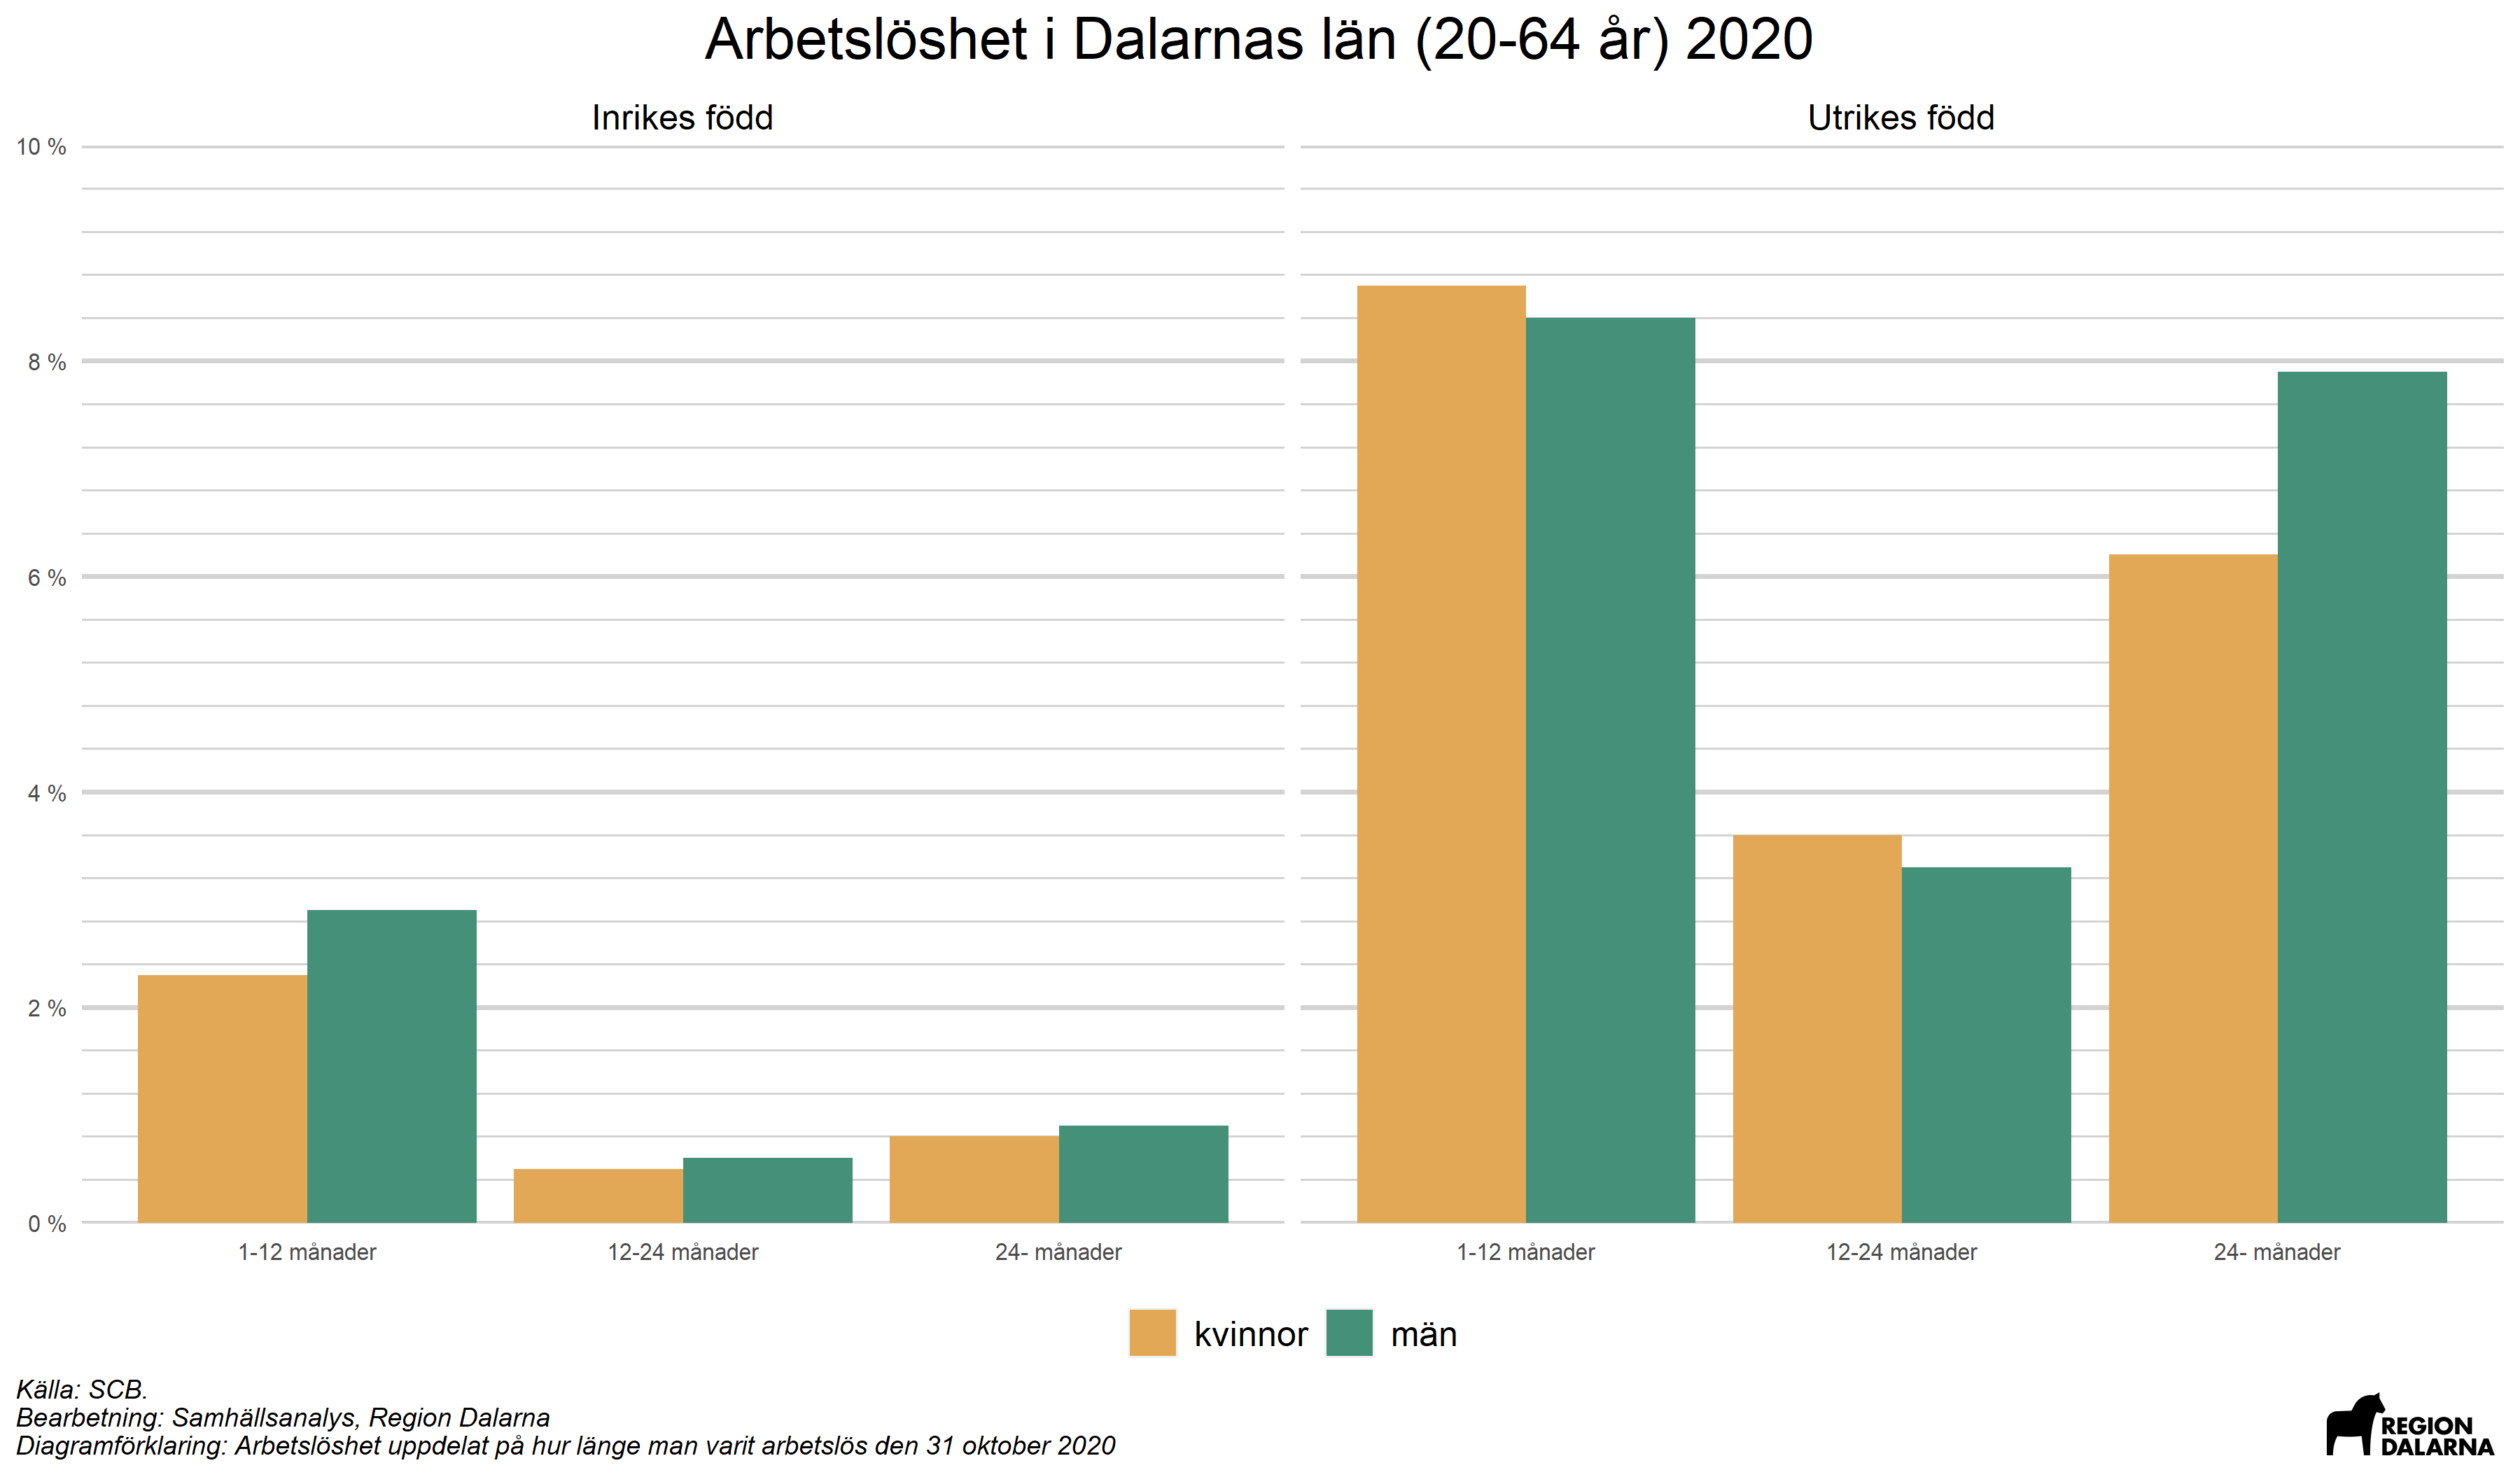
\includegraphics[width=0.9\linewidth]{G:/skript/projekt/kvinnor_man/Projekt_kvinnor_man/Diagram/langtidsarbetsloshet_lan_bakgrund} \end{center}

För att utöka bilden av arbetslösheten i länet redovisas här även
arbetslöshet efter utbildningsbakgrund för både kvinnor och män (se
figuren nedan). Arbetslösheten tenderar att vara lägre i grupper med
längre utbildning för både kvinnor och män. För gruppen med längst
utbildning, minst tre års eftergymnasial utbildning, ligger
kortidsarbetslösheten mellan 1 och 2 procent och långtidsarbetslösheten
är ännu lägre. I gruppen med lägst utbildning, förgymnasial utbildning
som är kortare än 9 år, ser vi däremot att arbetslösheten är betydligt
högre oavsett arbetslöshetstid.

\begin{center}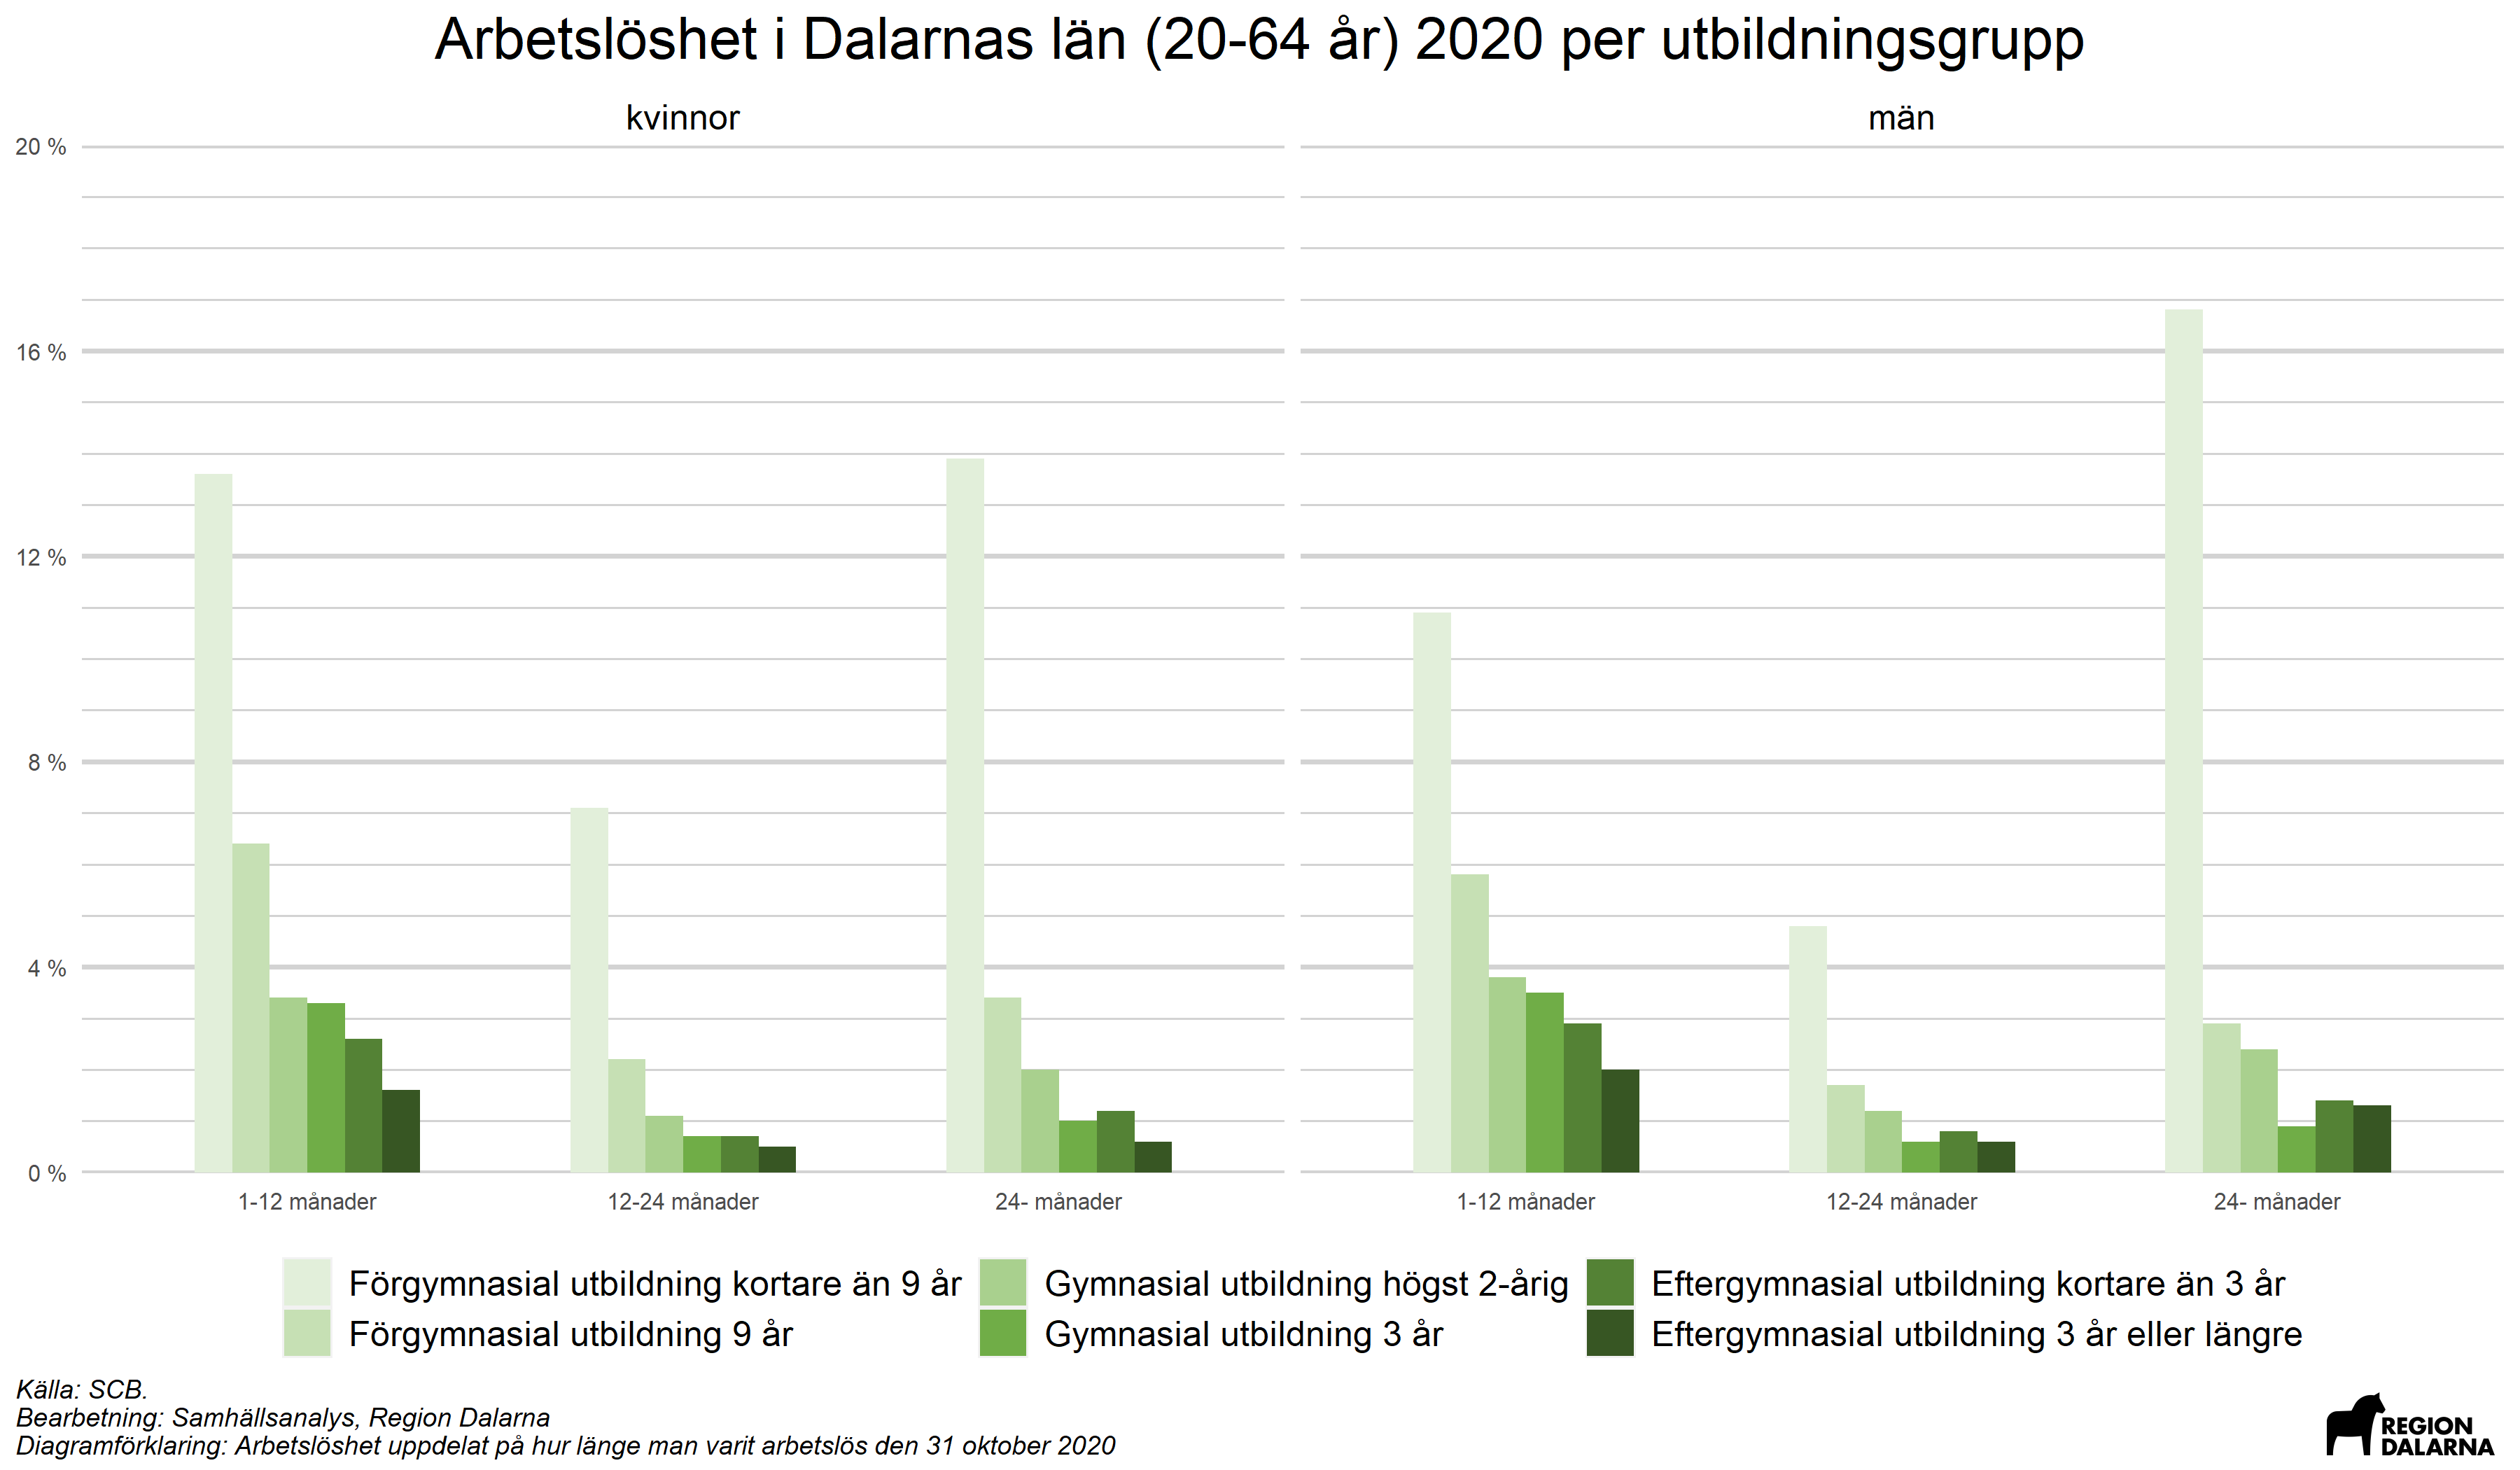
\includegraphics[width=0.9\linewidth]{G:/skript/projekt/kvinnor_man/Projekt_kvinnor_man/Diagram/langtidsarbetsloshet_lan_utbildningsniva} \end{center}

\hypertarget{matchning-puxe5-arbetsmarknaden}{%
\subsection{Matchning på
arbetsmarknaden}\label{matchning-puxe5-arbetsmarknaden}}

Nivån av matchning på arbetsmarknaden mäter i hur stor utsträckning
människor jobbar med vad de är utbildade till. Generellt tenderar olika
typer av specialicerade eftergymnasiala utbildningar, exempelvis läkare
och psykologer, ha hög matchning. Utbildar man sig till läkare är det
väldigt hög sannolikhet att man även har det som yrke (närmare 100
procent). På andra sidan av spektrumet finns dels olika former av
gymnasieutbildningar, dels eftergymansieala utbildningar inom exempelvis
humaniora och konst, där runt hälften jobbar med vad de är utbildade
till. Rent generellt ligger matchninggraden på runt 70 procent i
Sverige, där något fler kvinnor än män jobbar med vad de är utbildade
till. Det finns vissa skillnader mellan länen, men dessa är relativt
små. I Dalarna är matchningsgraden för såväl kvinnor som män strax under
70 procent, vilket är något sämre än riket som helhet.

\begin{center}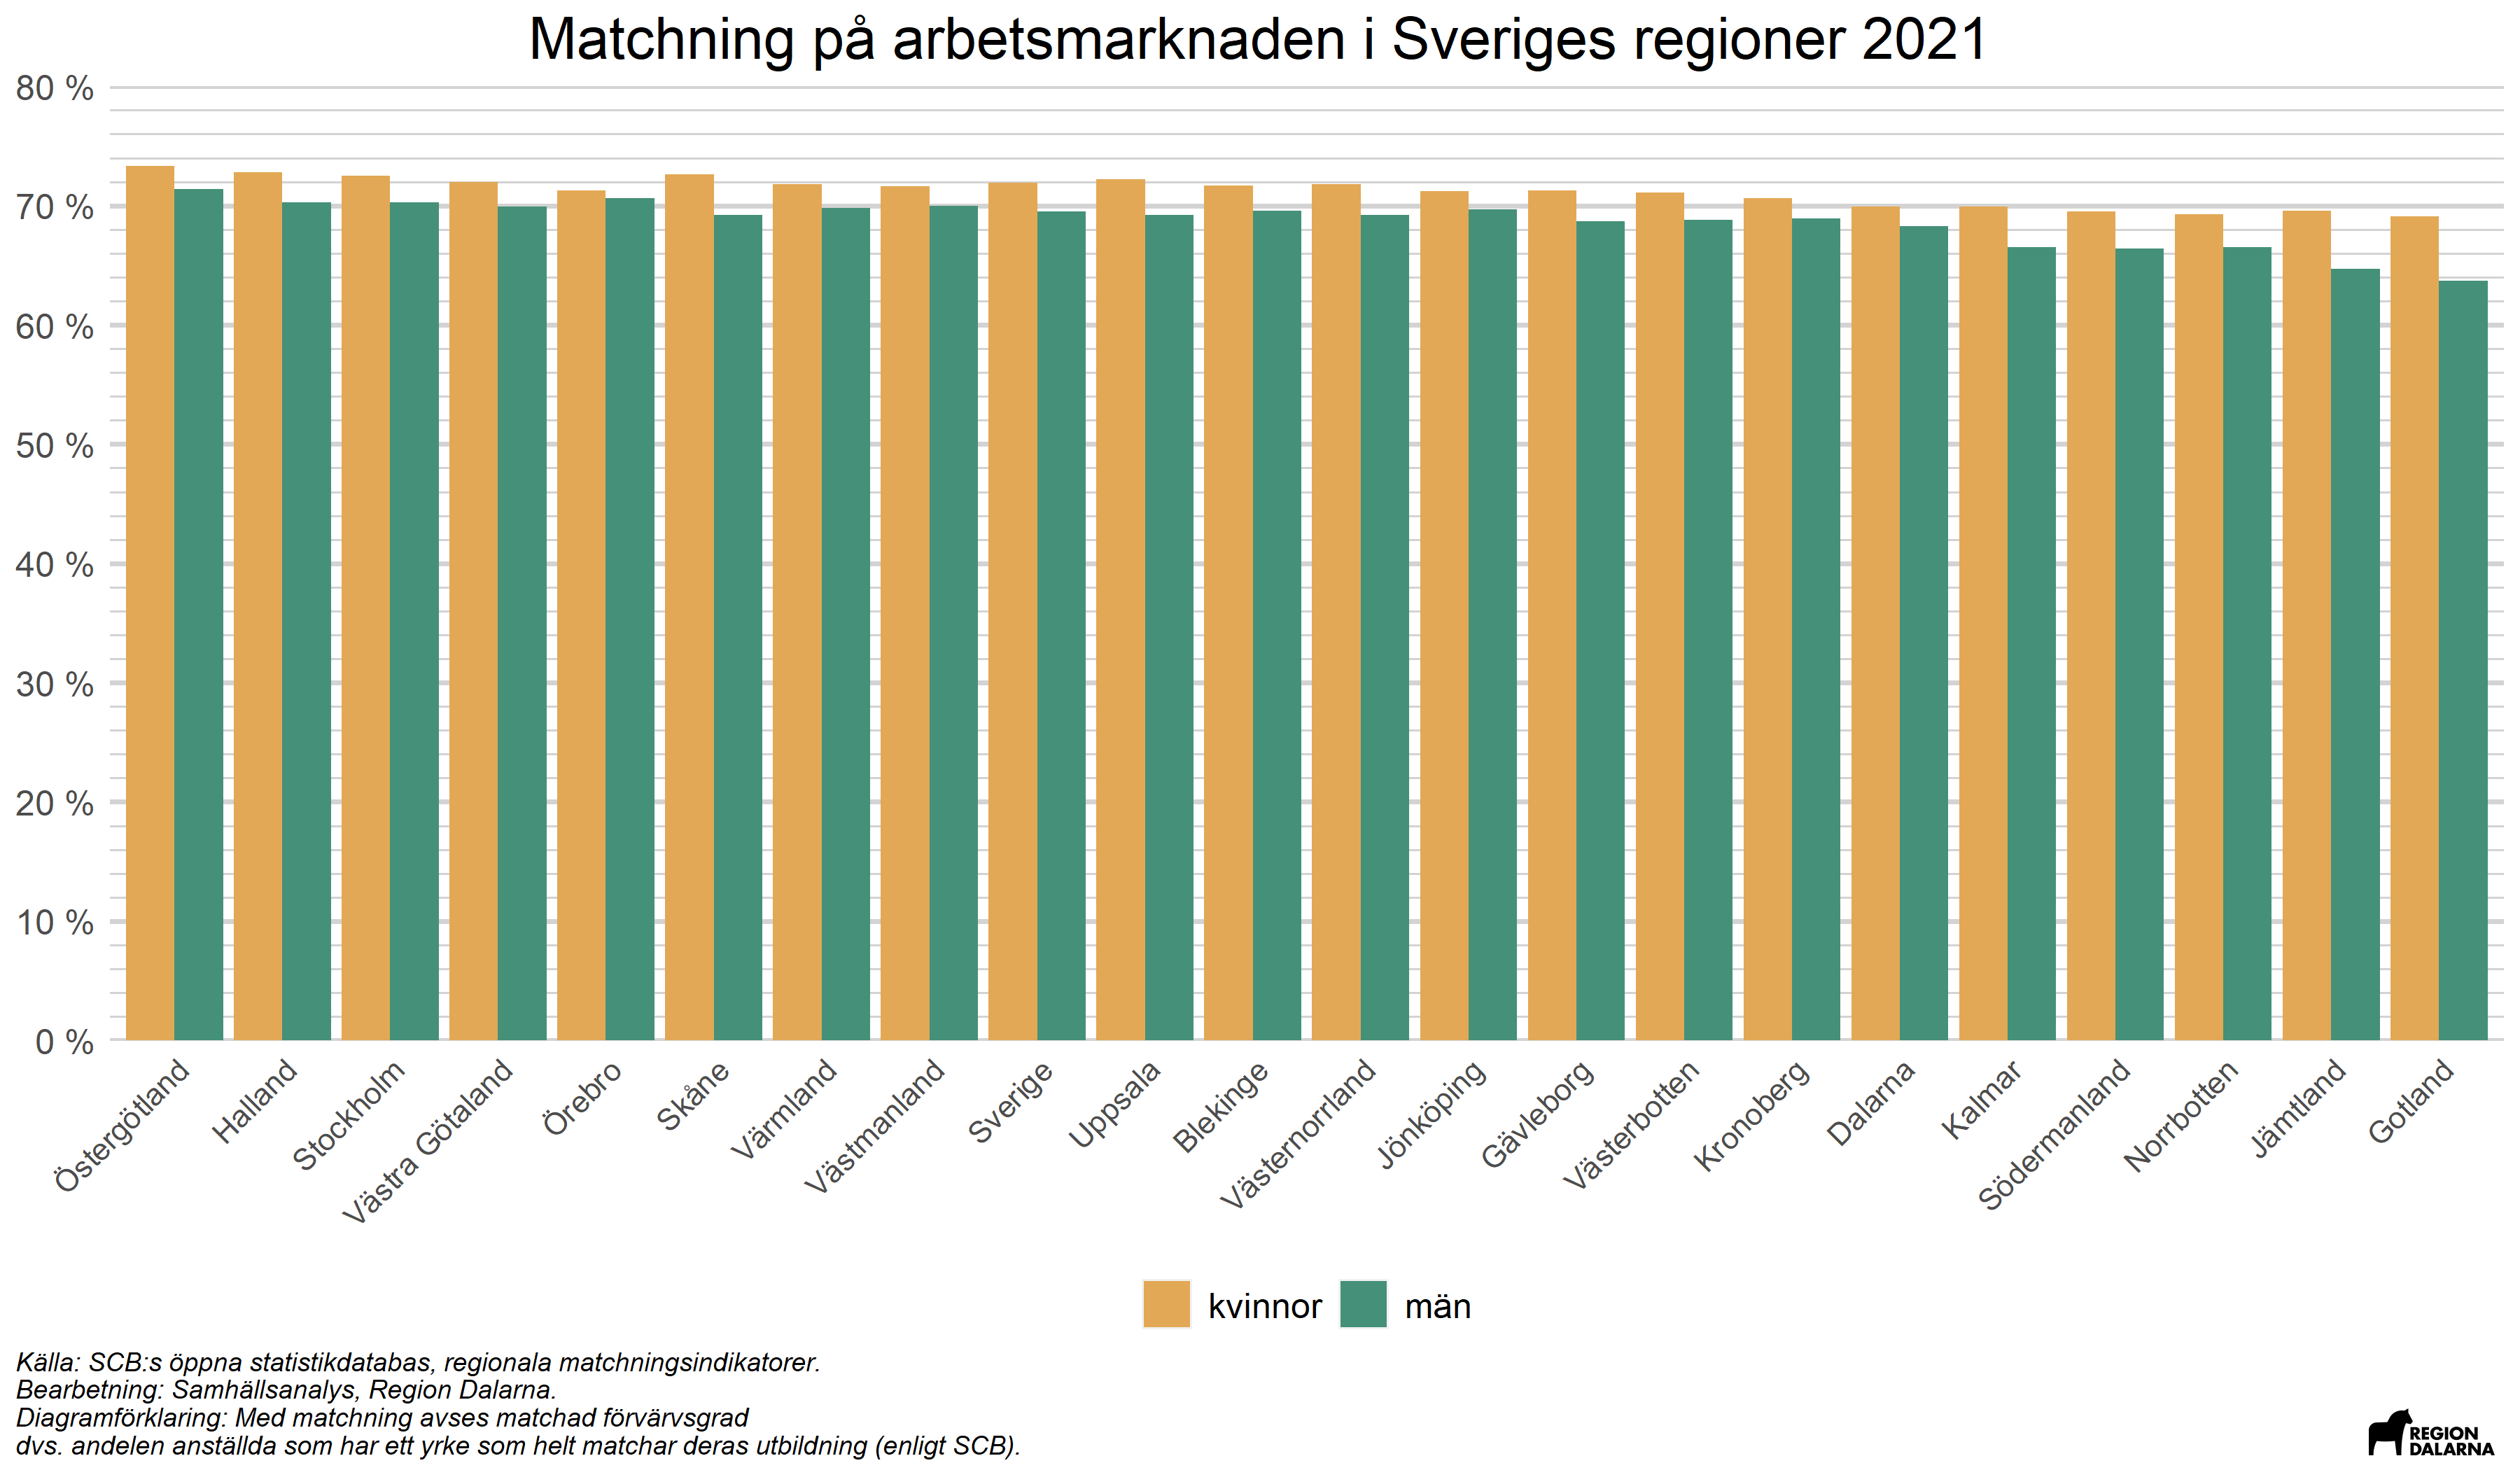
\includegraphics[width=0.9\linewidth]{G:/skript/projekt/kvinnor_man/Projekt_kvinnor_man/Diagram/matchning_lan} \end{center}

Matchningen på arbetsmarknaden tenderar att variera beroende på var man
är född. I Dalarna har inrikes födda högst matchning med närmare 70
procent för både kvinnor och män. Även personer födda inom EU har hög
matchning (runt 65 procent). Lägst matchningsgrad har personer födda i
Afrika (ca 60 procent).

\begin{center}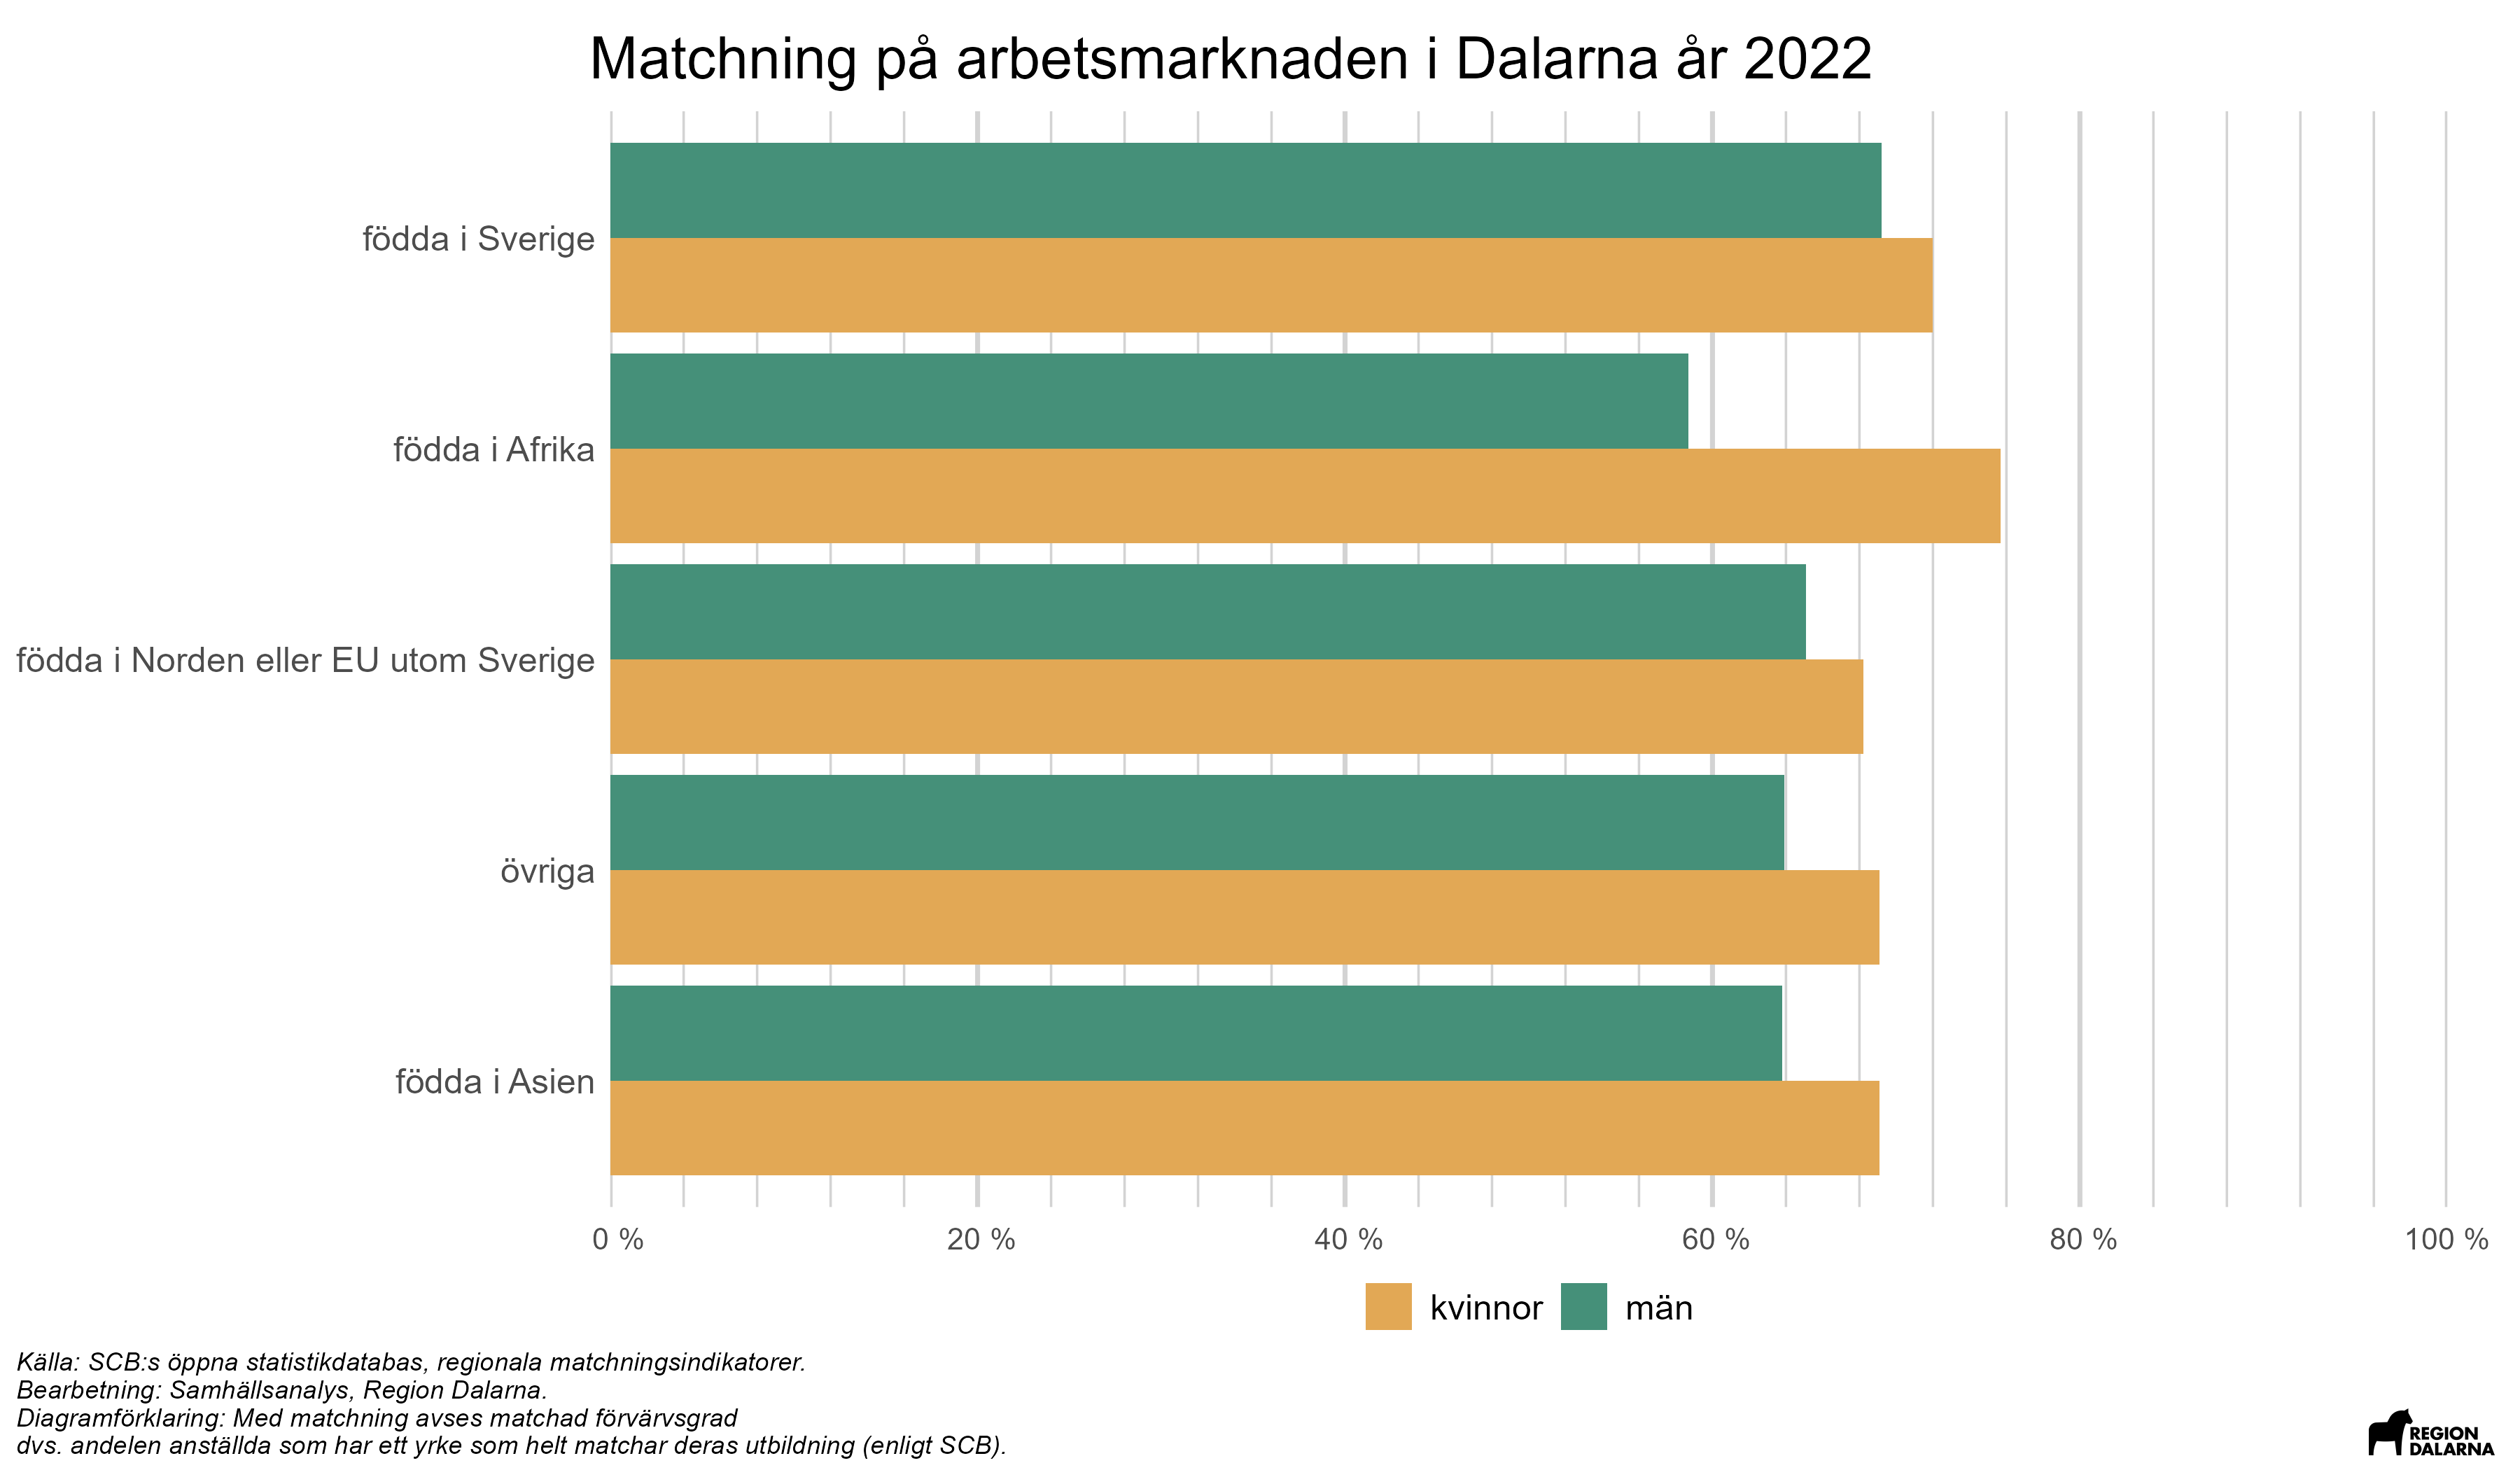
\includegraphics[width=0.9\linewidth]{G:/skript/projekt/kvinnor_man/Projekt_kvinnor_man/Diagram/matchning_bakgrund} \end{center}

\hypertarget{etablering}{%
\subsection{Etablering}\label{etablering}}

Som diskuterats tidigare är sysselsättningsgraden låg bland utrikes
födda generellt, och framförallt bland kvinnor. En bidragande orsak till
det är att det tar relativt lång tid för, i första hand, nyanlända
kvinnor att etablera sig på arbetsmarknaden. För utrikesfödda kvinnor
som befunnit sig i Sverige i upp till 2 år (0-1 år i grafen nedan) är de
bara knappt en fjärdedel i arbetsför ålder (20-64 år) som arbetar. För
motsvarande grupp bland männen arbetar ungefär varannan inom 2 år. Över
tid tenderar etableringsgraden att öka avsevärt och efter minst tio år i
Sverige är det ungefär 70 procent av såväl männen som kvinnorna som
arbetar.

\begin{center}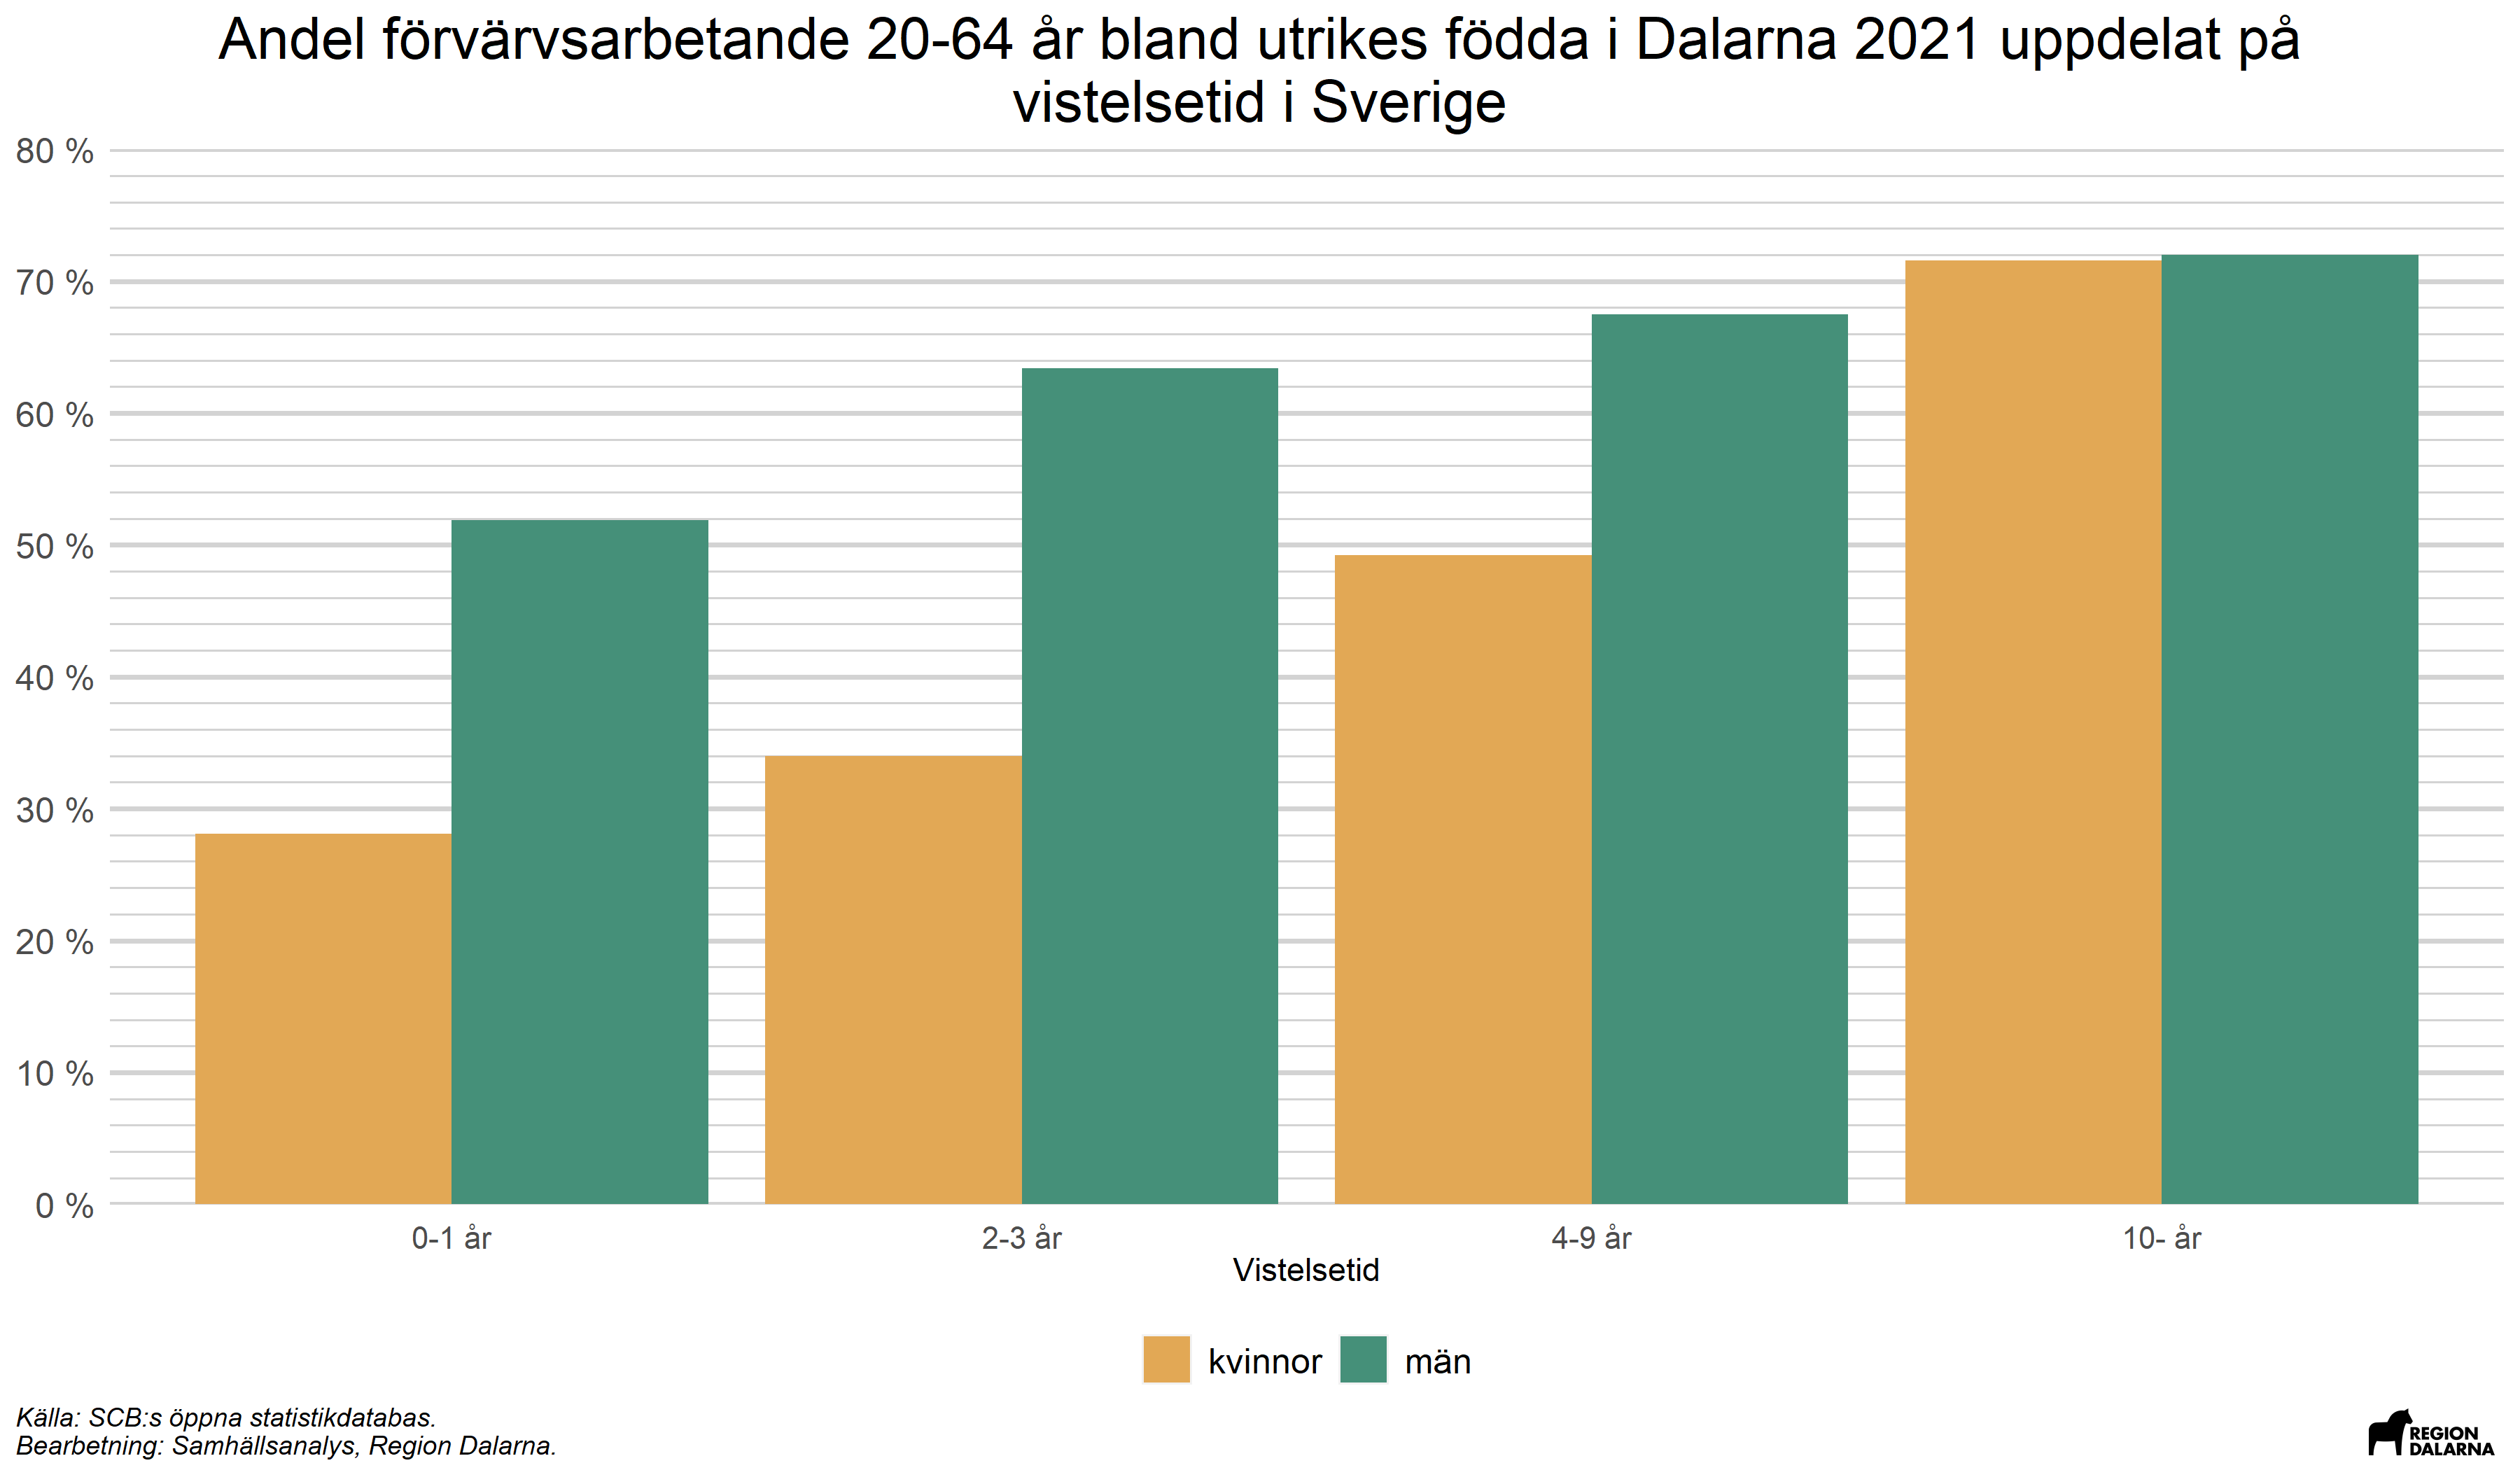
\includegraphics[width=0.9\linewidth]{G:/skript/projekt/kvinnor_man/Projekt_kvinnor_man/Diagram/etablering_lan} \end{center}

Hur snabbt en nyanländ person etableras på arbetsmarknaden är nära
kopplat till vilken utbildningsnivå personen har. För de med högst
utbilning tenderar processen att gå relativt snabbt och nära 40 procent
av kvinnorna och 60 procent av männen arbetar innan man varit i Sverige
i 2 år (0-1 år i figuren nedan). Sedan ökar etableringsgraden över tid
och efter 10 år eller längre har fler än 80 procent av kvinnorna mellan
20 år och 64 år jobb, vilket är i linje med sysselsättningsgraden för
inrikes födda kvinnor i samma åldersgrupp. För de med lägst utbildning
(ej gymnasieutbildning) är situationen väsentligt annorlunda. I den
gruppen jobbar ungefär var 10e utrikesfödd kvinna, och var 3e
utrikesfödd man, inom 2 år efter att man kommit till Sverige. Över tid
ökar etableringen på arbetsmarknaden, men bara ungefär hälften av
kvinnorna och ungefär 60 procent av männen jobbar trots att de varit i
Sverige i minst 10 år.

\begin{center}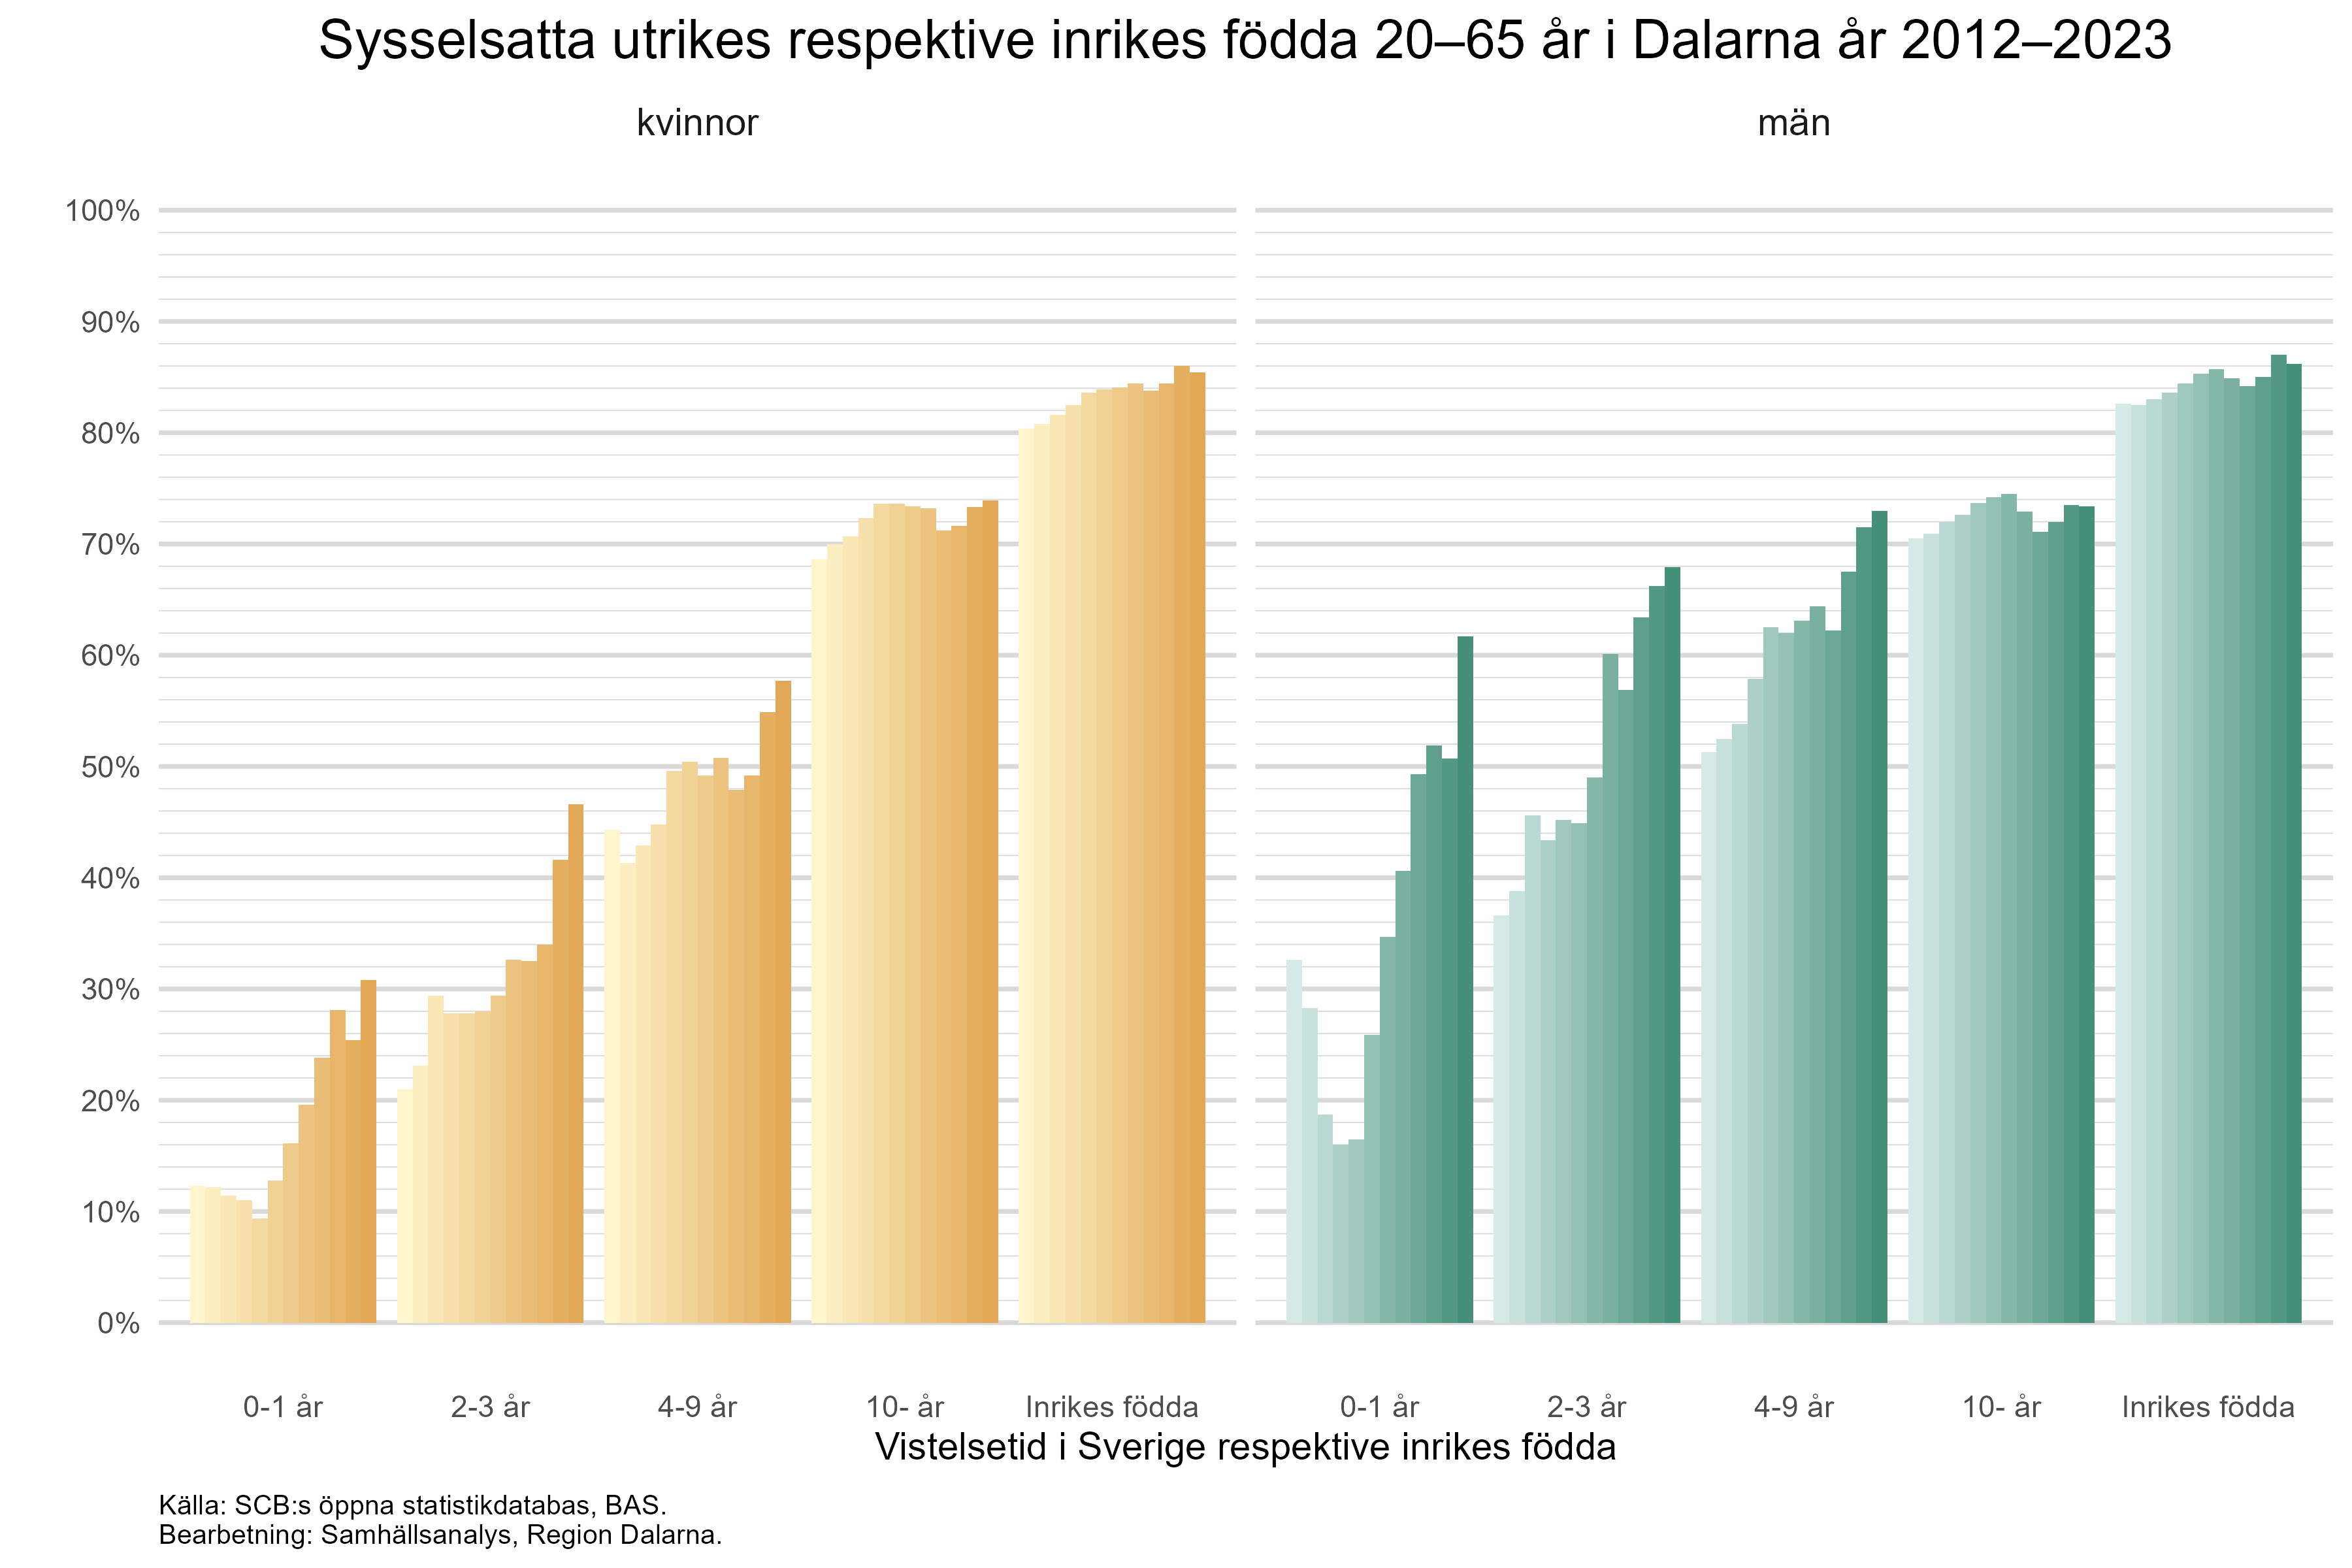
\includegraphics[width=0.9\linewidth]{G:/skript/projekt/kvinnor_man/Projekt_kvinnor_man/Diagram/etablering_lan_utb} \end{center}

\hypertarget{ekonomisk-juxe4mstuxe4lldhet}{%
\section{Ekonomisk jämställdhet}\label{ekonomisk-juxe4mstuxe4lldhet}}

\hypertarget{inkomst}{%
\subsection{Inkomst}\label{inkomst}}

En jämförelse av kvinnor och mäns löner i Dalarna visar på stora
skillnader som har hållit i sig över tid. Medianinkomsten för en man i
Dalarna var 2020 strax över 360 000 kr före skatt, medan en kvinna hade
en medianinkomst på drygt 300 000 kr. I den andra figuren nedan syns
dock att den relativa skillnaden i inkomst mellan könen har minskat
sedan millenieskiftet. Diagrammet visar att kvinnans medianinkomsten har
fördubblats medan mannens har ökat med ungefär 80 procent. Det är dock
viktigt att notera att figurerna nedan inte tar hänsyn till andra
faktorer än kön som kan tänkas förklara inkomstens storlek. Som vi sett
i ett flertal tidigare figurer finns det stora skillnader mellan könen
kopplat till bland annat yrke och utbildning, vilket kan förklara en del
av skillnaden. På nationell nivå har SCB jämfört den standardvägda
lönen, dvs. lönen när man tagit hänsyn till bland annat ålder och
utbildningsnivå, mellan könen och kommit fram till att kvinnors
standardvägda lön är ungefär 95\% av männens standardvägda lön
\footnote{SCB:
  \url{https://www.scb.se/hitta-statistik/statistik-efter-amne/arbetsmarknad/loner-och-arbetskostnader/lonestrukturstatistik-hela-ekonomin/pong/tabell-och-diagram/kvinnors-lon-i-procent-av-mans-lon-efter-sektor}}

\begin{center}\includegraphics[width=0.9\linewidth]{G:/skript/projekt/kvinnor_man/Projekt_kvinnor_man/Diagram/medianinkomst_kon_total_Dalarnas län} \end{center}

\begin{center}\includegraphics[width=0.9\linewidth]{G:/skript/projekt/kvinnor_man/Projekt_kvinnor_man/Diagram/medianinkomst_kon_total_forandring_Dalarnas län} \end{center}

Utöver inkomster är det även relevant att undersöka den disponibla
inkomsten, dvs. summan av alla inkomster och transfereringar (exempelvis
barnbidrag) minus slutgiltig skatt. I figuren nedan är det tydligt att
den disponibla inkomsten varierar mellan olika grupper. En generell
trend för alla grupper är att den disponibla inkomsten, utan att justera
för inflation, har ökat mellan 2011-2020.

Det är tydligt att sammanboende, med eller utan barn, har en högre
disponibel inkomst än ensamstående. Sammanboende med barn har också en
högre disponibel inkomst än sammanboende utan barn. På andra sidan av
skalan återfinns gruppen ensamstående kvinnor utan barn som har lägst
disponibel inkomst. Diagrammet visar också på att det finns tydliga
skillnader mellan könen. Bland ensamstående har män, med eller utan
barn, högre disponibel inkomst än kvinnor i motsvarande grupp.

\begin{center}\includegraphics[width=0.9\linewidth]{G:/skript/projekt/kvinnor_man/Projekt_kvinnor_man/Diagram/disponibel_inkomstDalarnas län} \end{center}

\hypertarget{antal-skuldsatta}{%
\subsection{Antal skuldsatta}\label{antal-skuldsatta}}

Ytterligare en aspekt av ekonomisk status är skuldsättningsgraden för
olika grupper. I det första diagrammet nedan redovisas antalet personer
i Dalarna som har skulder under indrivning hos Kronofogden. Två trender
är tydliga. Under det senaste decenniet har antalet skuldsatta minskat
från drygt 10 000 skuldsatta till drygt 8000 i Dalarnas län. Det är
också en tydlig variation mellan kvinnor och män, där den senare gruppen
har avsevärt fler skuldskatta i länet.

I det andra diagrammet nedan redovisas antalet långsiktigt skuldsatta i
Dalarna. Även här finns det betydligt fler män än kvinnor. Över tid
skedde en svag ökning av antalet långsiktigt skuldsatta i åren i början
på tidsperioden för att sjunka tillbaka under de senare åren som är
inkluderade i diagrammet.

\begin{center}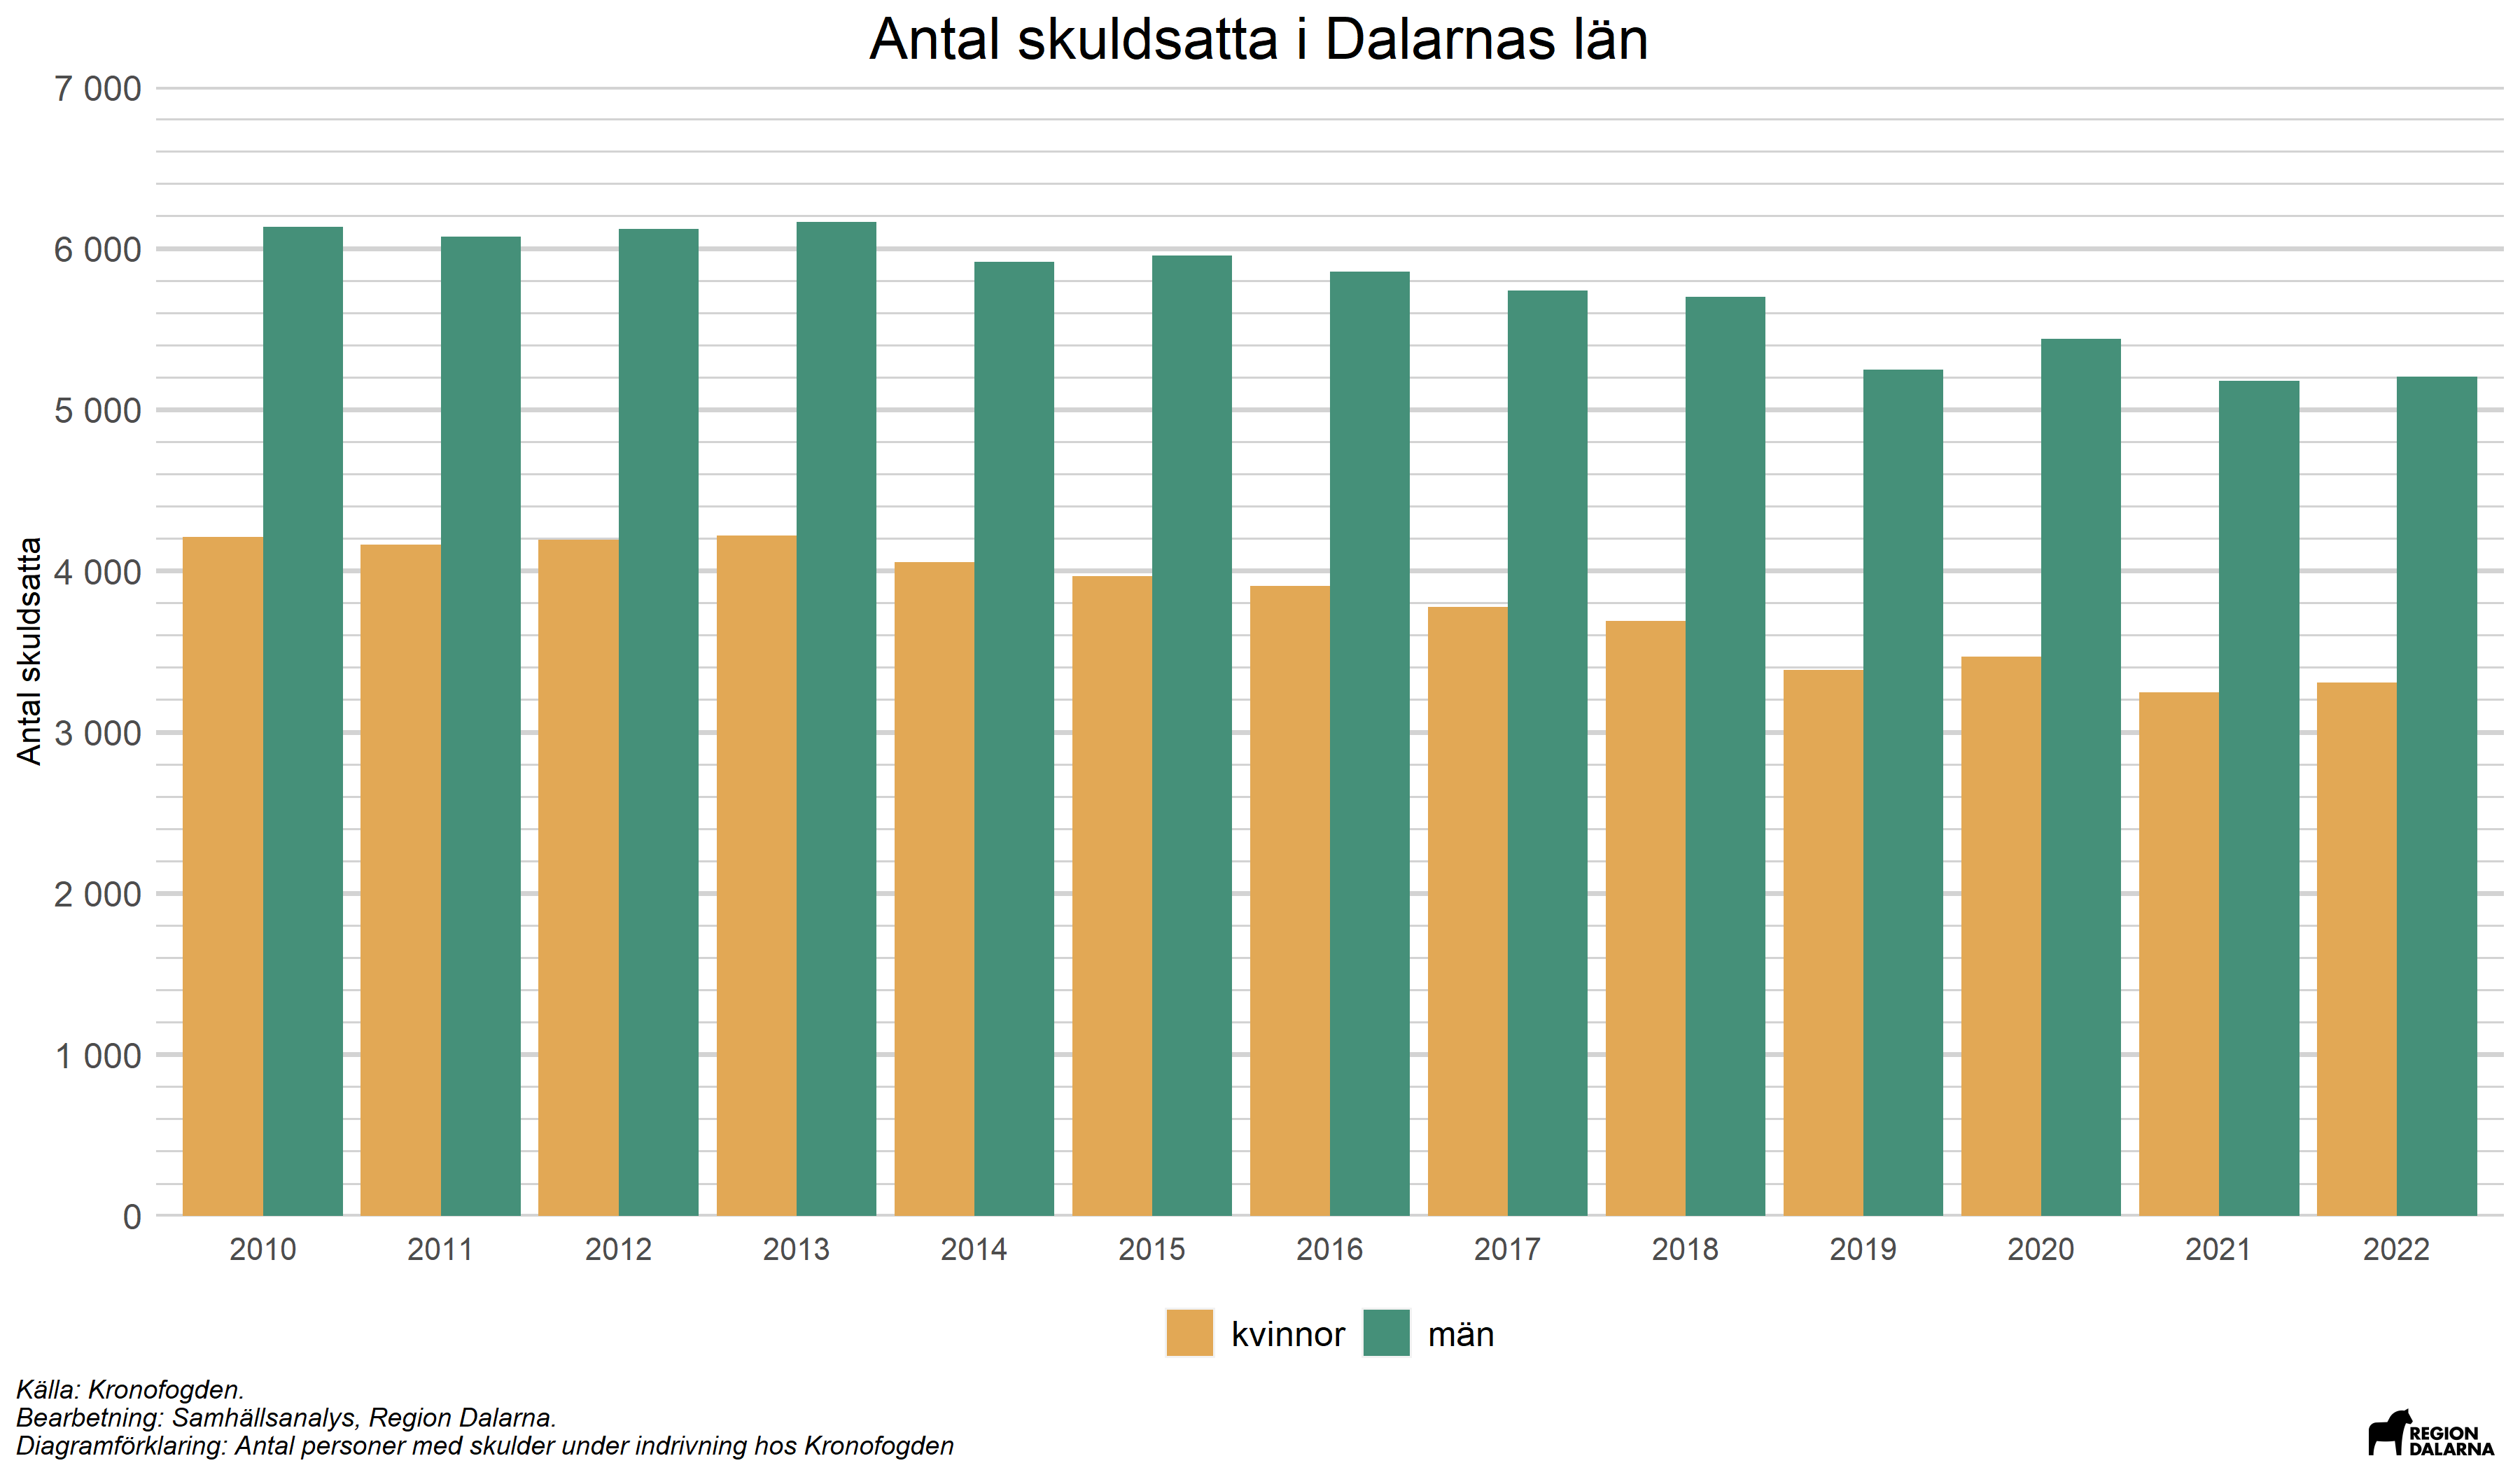
\includegraphics[width=0.9\linewidth]{G:/skript/projekt/kvinnor_man/Projekt_kvinnor_man/Diagram/antal_skuldsatta_Dalarna} \end{center}

\begin{center}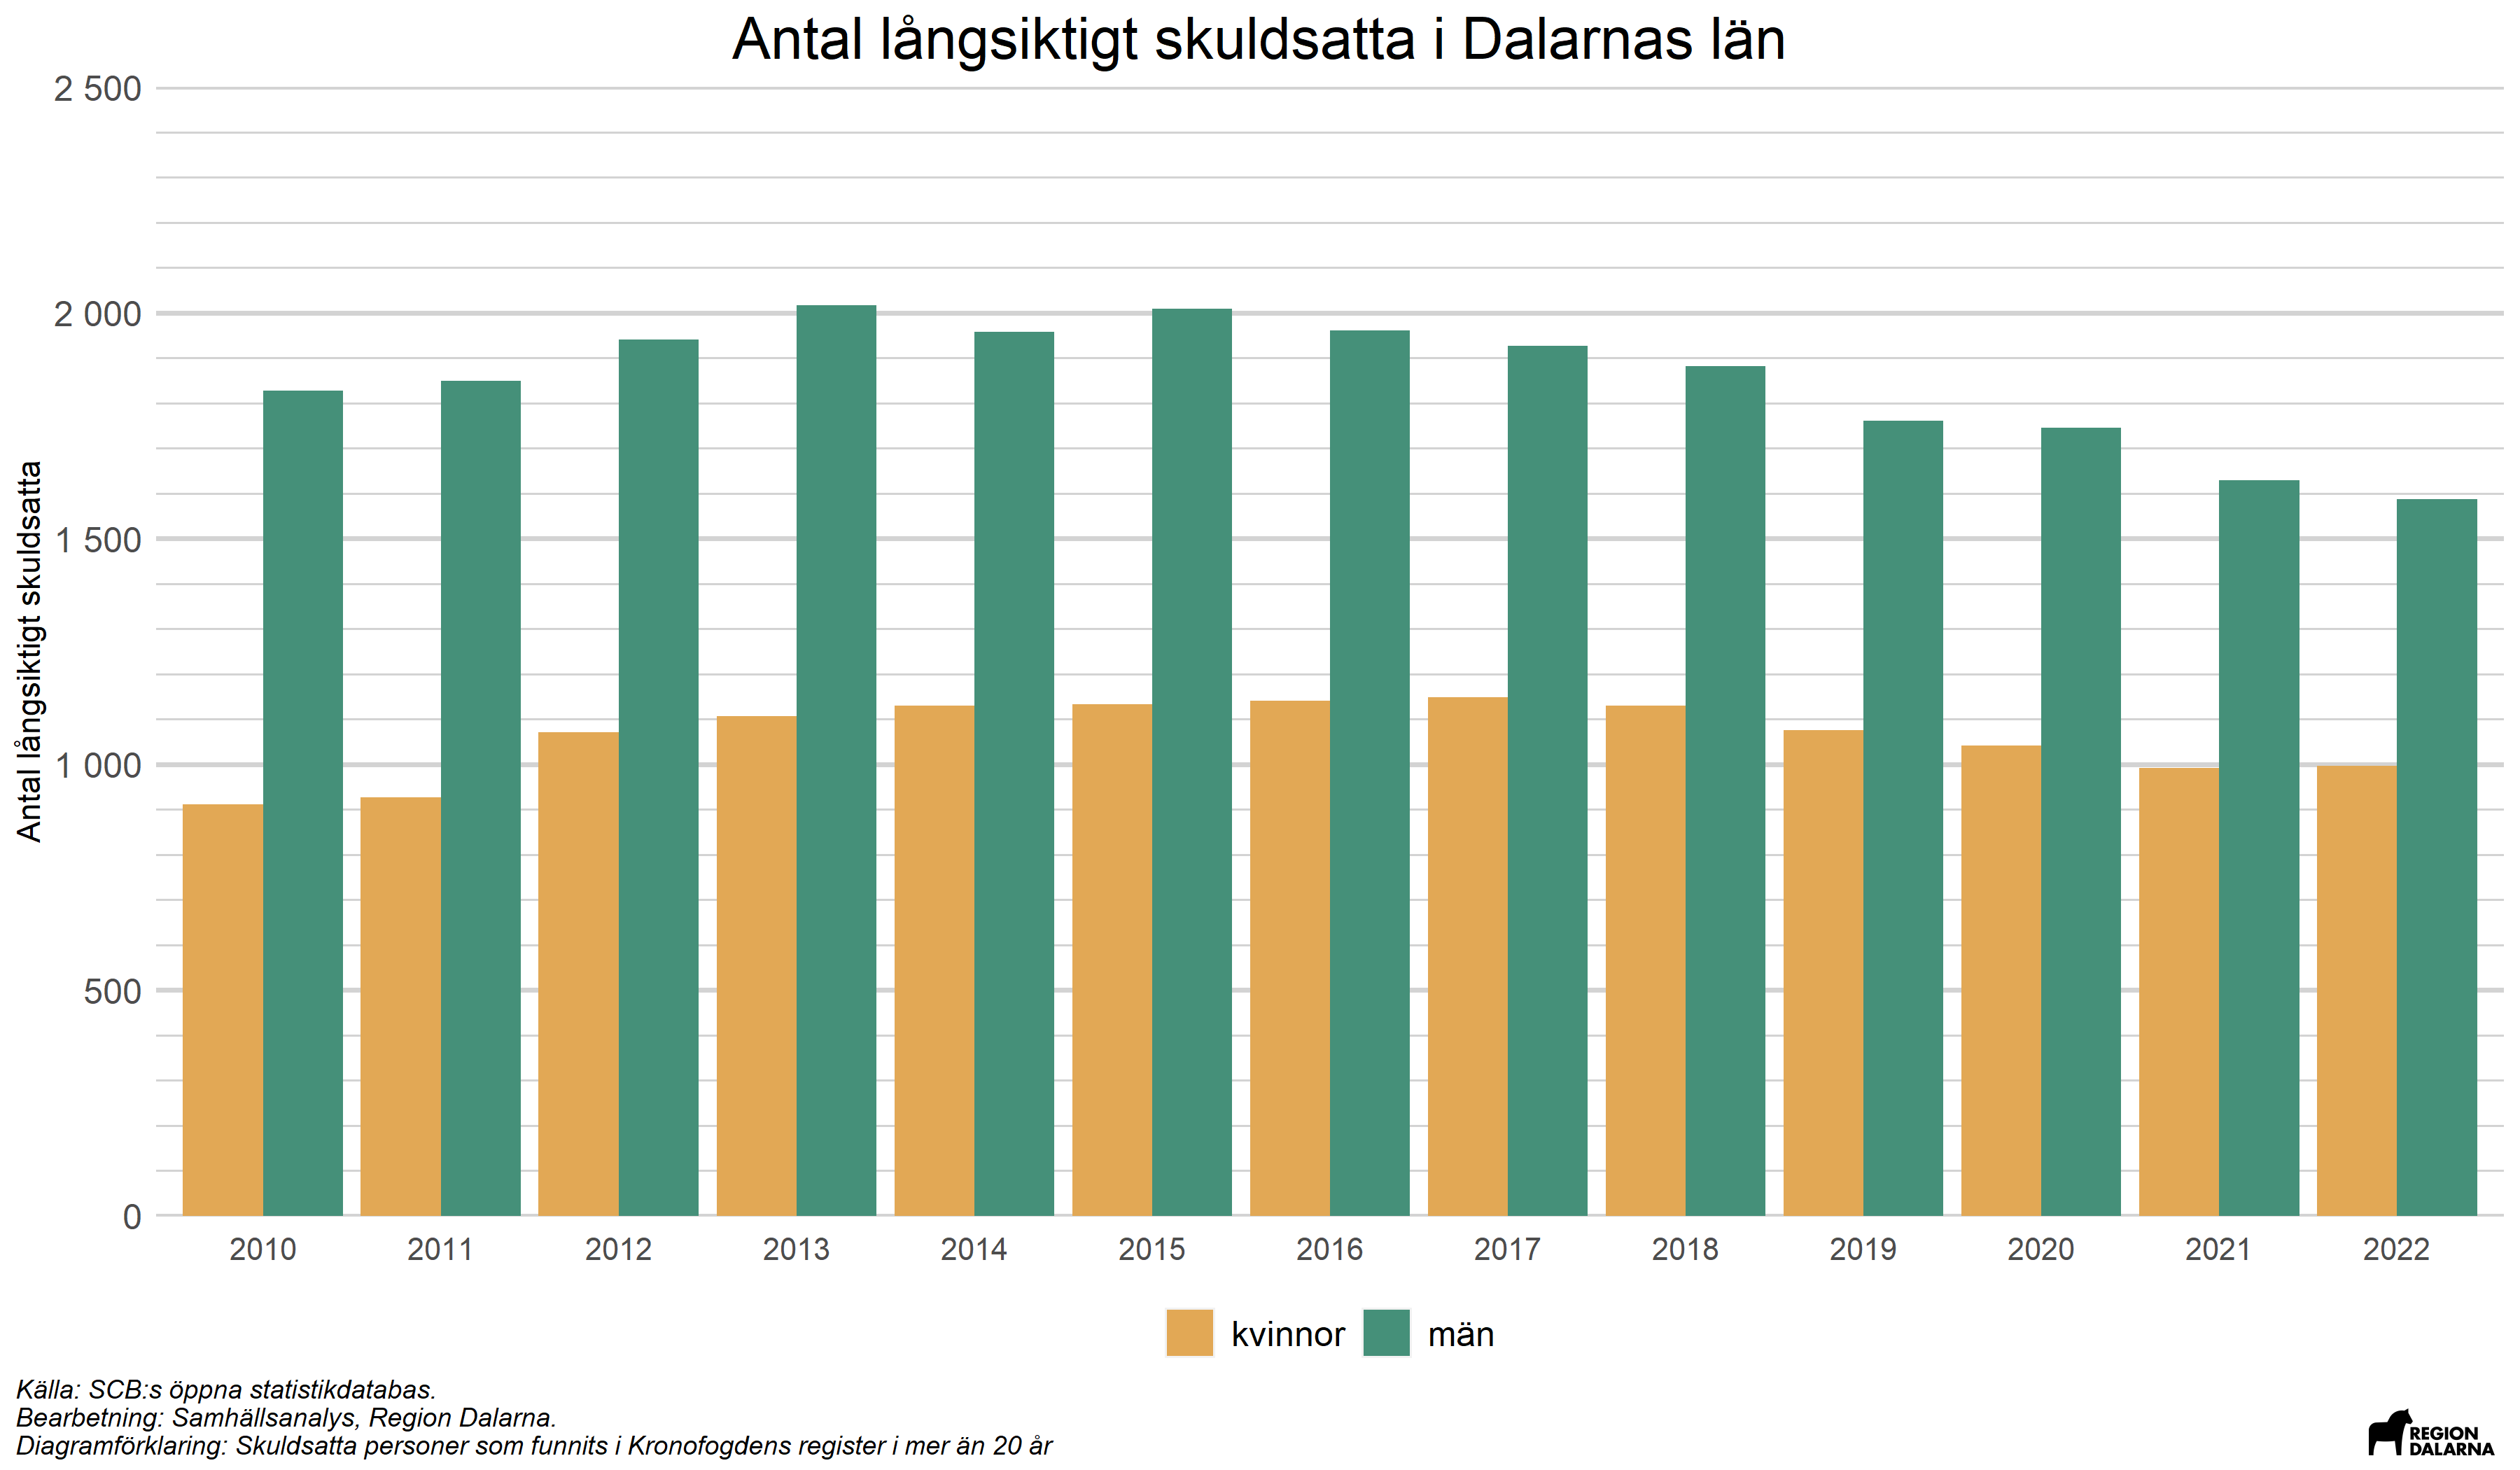
\includegraphics[width=0.9\linewidth]{G:/skript/projekt/kvinnor_man/Projekt_kvinnor_man/Diagram/Antal_langsiktigt_skuldsatta} \end{center}

\hypertarget{ohuxe4lsa}{%
\section{(O)hälsa}\label{ohuxe4lsa}}

\hypertarget{ohuxe4lsotalet}{%
\subsection{Ohälsotalet}\label{ohuxe4lsotalet}}

Det finns tydliga skillnader mellan kvinnor och män inom hälsa.
Ohälsotalet\footnote{Ohälsotalet: hur många dagar under en
  tolvmånadersperiod Försäkringskassan betalar ut ersättning för nedsatt
  arbetsförmåga i förhållande till antalet försäkrade i åldrarna 16-64
  år.} mäter utsträckningen i vilken personer tvingas vara borta från
jobbet under längre perioder på grund av nedsatt arbetsförmåga.
Ohälsotalet varierar över tid och var relativt högt under början av
00-talet. Därefter syns en klart nedåtgående trend. Under hela
tidsperioden har ohälsotalet varit högre för kvinnor än för män även om
skillnaden mellan könen har minskat något över tid.

Inom Dalarna visar ohälsotalet att det finns skillnader mellan länets
kommuner. För män är ohälsotalet högst i Hedemora och lägst i Falun. För
kvinnor är ohälsotalet högst i Rättvik och lägst i Leksand. Skillnaden
mellan kvinnor och män högst i Rättvik. Orsaken till skillnaderna
behöver djupare studier och analys men potentiella faktorer omfattar
dels branschstrukturen i olika kommuner och dels socioekonomiska
variabler som skiljer mellan kommunerna i Dalarna.

\begin{center}\includegraphics[width=0.9\linewidth]{G:/skript/projekt/kvinnor_man/Projekt_kvinnor_man/Diagram/ohalsotalDalarnas län} \end{center}

\begin{center}\includegraphics[width=0.9\linewidth]{G:/skript/projekt/kvinnor_man/Projekt_kvinnor_man/Diagram/ohalsotal_kommunDalarnas län} \end{center}

\hypertarget{sjukpenningtalet}{%
\subsection{Sjukpenningtalet}\label{sjukpenningtalet}}

I likhet med ohälsotalet så tenderar sjukpenningtalet, som enbart
innefattar sjukpenning och rehabiliteringspenning, att variera kraftigt
över tiden. I början av 00-talet var talet högt för både kvinnor och
män, för att därefter minska rejält fram till 2010. Därefter kan en
ökning återigen skönjas, innan sjukpenningtalet stabiliserats på senare
år. Kvinnor är sjukskrivna i större utsträckning än män, vilket
återspeglas i sjukpenningtalet. Att talet förändras över tid behöver
inte nödvändigtvis bero på att människor blir mer eller mindre sjuka.
Det kan snarare bero på en mer eller mindre restriktiv syn på vad som
krävs för att bli sjukskriven, något som ofta är politiskt påverkat.
Exempelvis beror den kraftiga nedgången i sjukpenningtalet mellan 2002
och 2010 sannolikt inte på att arbetstagare var mindre sjuka, utan på
att bedömningen av vad som berättigar en sjukskrivning var hårdare.

Även när det kommer till sjukpenningtalet finns det skillnader mellan
Dalarnas kommuner. För män är talet högst i Rättvik, medan det för
kvinnor är högst i Säter. Precis som var fallet vid ohälsotalet
tidigare, är Falun återigen bäst i klassen, denna gång för såväl kvinnor
som män.

\begin{center}\includegraphics[width=0.9\linewidth]{G:/skript/projekt/kvinnor_man/Projekt_kvinnor_man/Diagram/SjukpenningtalDalarnas län} \end{center}

\begin{center}\includegraphics[width=0.9\linewidth]{G:/skript/projekt/kvinnor_man/Projekt_kvinnor_man/Diagram/Sjukpenningtal_kommunDalarnas län} \end{center}

\hypertarget{stress}{%
\subsection{Stress}\label{stress}}

En märkbar utveckling under de senaste årtiodena är ökningen i antalet
stressrelaterade sjukskrivningar. Ett allt större antal sjukskrivningar,
för både män och kvinnor, kan kopplas till stress i Dalarna. För kvinnor
har antalet pågående sjukfall kopplade till stress mellan 2009 och 2016
tiodubblats. Från 2016 till idag har utvecklingen stabiliserats men
ligger kvar på en mycket högre nivå än innan uppgången påbörjades.
Antalet män som sjukskriver sig med hänvisning till stress har också
ökat, om än inte i lika stor utsträckning som den för kvinnor. Att
utröna exakt vad detta beror på är svårt, men det finns ett väl belagt
samband mellan psykiatriska diagnoser (såsom svår stress) och den
psykosociala arbetsmiljön.\footnote{Försäkringskassan, Korta analyser
  2016:2, `'Sjukskrivning för reaktioner på svår stress ökar mest.'':
  \url{https://www.forsakringskassan.se/download/18.3a5418591814e228e4413b2/1661267958656/psykisk-ohalsa-korta-analyser-2016-2.pdf}}

\begin{center}\includegraphics[width=0.9\linewidth]{G:/skript/projekt/kvinnor_man/Projekt_kvinnor_man/Diagram/Antal_stressDalarnas län} \end{center}

\hypertarget{uxe4r-det-skillnader-puxe5-branscher}{%
\subsection{Är det skillnader på
branscher?}\label{uxe4r-det-skillnader-puxe5-branscher}}

Rent generellt är det stora skillnader i antalet startade sjukfall (per
1000 förvärvsarbetande) mellan olika branscher. För kvinnor är antalet
störst i typiskt kvinnodominerade yrken som vård och omsorg och
utbildning, vilket kan vara en förklaring till att kvinnor är
sjukskrivna i större utsträckning än män. För män är det istället inom
transport som antalet startade sjukfall är högst. Oavsett kön, är antal
startade sjukfall lägst inom klassiska kontorsjobb som ekonomi, juridik
och IT.

\begin{center}\includegraphics[width=0.9\linewidth]{G:/skript/projekt/kvinnor_man/Projekt_kvinnor_man/Diagram/Startade_sjukfall_branschDalarnas län} \end{center}

\hypertarget{obetalt-arbete}{%
\section{Obetalt arbete}\label{obetalt-arbete}}

\hypertarget{fuxf6ruxe4ldrapenning}{%
\subsection{Föräldrapenning}\label{fuxf6ruxe4ldrapenning}}

Antalet mottagare av föräldrapenning (den första figuren nedan) har ökat
från ungefär 13 000 i slutet av 90-talet för att nå upp över 22 000
under 2018. En viss minskning syntes under pandemiåren, vilket sannolikt
beror på att uttaget av tillfällig föräldrapenning (VAB) då ökade
kraftigt (se nedan). Antalet uttagna dagar har ökat för såväl kvinnor
som män, men den relativa skillnaden i uttag mellan könen har minskat. I
slutet av 90-talet togs runt 85-90 procent av föräldrapenning ut av
mammorna, en andel som hade minskat till runt 70 procent 2021.
Utvecklingen går dock relativt trögt och Sverige är långt ifrån ett
jämställt uttag av dagar.

Antalet mottagare av föräldrapenning är olika jämnt fördelade beroende
på vilken kommun i Dalarna vi tittar på. Falun är relativt mest
jämställt, där över 30\% av föräldrapenningen togs ut av männen. Minst
jämställt är Orsa, där motsvarande uttag är ungefär 20\%.

\begin{center}\includegraphics[width=0.9\linewidth]{G:/skript/projekt/kvinnor_man/Projekt_kvinnor_man/Diagram/Foraldrapenning_antalDalarnas län} \end{center}

\begin{center}\includegraphics[width=0.9\linewidth]{G:/skript/projekt/kvinnor_man/Projekt_kvinnor_man/Diagram/Foraldrapenning_andelDalarnas län} \end{center}

\begin{center}\includegraphics[width=0.9\linewidth]{G:/skript/projekt/kvinnor_man/Projekt_kvinnor_man/Diagram/Foraldrapenning_andel_kommunDalarnas län} \end{center}

\hypertarget{tillfuxe4llig-fuxf6ruxe4ldrapenning}{%
\subsection{Tillfällig
föräldrapenning}\label{tillfuxe4llig-fuxf6ruxe4ldrapenning}}

Vad gäller tillfällig föräldrapenning, det som i folkmun kallas Vab,
minskade antalet uttagna nettodagar något mellan 2006 och 2009, för att
därefter öka stadigt fram till idag (den första figuren nedan). En
tydlig pandemieffekt går att skönja, då antalet dagar ökade avsevärt
från 2019 till 2020/2021. Kvinnor tar ut betydligt fler dagar än männen,
men till skillnad från föräldrapenning blir uttaget av Vab-dagar inte
mer jämställt över tiden (det verkar dock föreligga en viss skillnad
under pandemin), se den andra figuren nedan

\begin{center}\includegraphics[width=0.9\linewidth]{G:/skript/projekt/kvinnor_man/Projekt_kvinnor_man/Diagram/Vab_antalDalarnas län} \end{center}

\begin{center}\includegraphics[width=0.9\linewidth]{G:/skript/projekt/kvinnor_man/Projekt_kvinnor_man/Diagram/Vab_antal_linjeDalarnas län} \end{center}

\hypertarget{makt-och-politik}{%
\section{Makt och politik}\label{makt-och-politik}}

\hypertarget{politiskt-valda}{%
\subsection{Politiskt valda}\label{politiskt-valda}}

Den politiska sfären har historiskt varit mansdominerad och kvinnor har
haft avsevärt färre tynga politiska uppdrag. Det första diagrammet i det
här avsnittet visar könsfördelningen bland riksdagsledamöter från valet
1973 till 2018. Riksdagens könsfördelning har under den här tidsperioden
sett en stor förändring och utveckling. Vid riksdagsvalet 1973 var en
övervägande majoritet av de folkvalda ledamöterna män. Endast drygt 70
kvinnor återfanns på bänkarna i Riksdagen under den här mandatperioden.
45 år senare är männen fortfarande fler än kvinnorna, men skillnaden
mellan könen är färre än 30 stycken ledamöter. Den mest jämställda
Riksdagen i Sverige var mandatperioden 2006-2010 då antalet kvinnor
översteg 160.

Trenden på nationell nivå syns även på regional nivå där trenden går mot
mer jämställdhet bland de folkvalda. Vid landstingsvalet 1982 i Dalarna
var antalet manliga ledamöter i regionfullmäktige övervägande män. Vid
regionvalet 2014 var fördelning i princip helt jämställd med nästan
samma antal män och kvinnor bland folkvalda i regionens fullmäktige.
Efter valet 2018 syns däremot återigen en ökning av antalet män i
Regionfullmäktige.

På lokal nivå i Dalarna finns det stora skillnader mellan kommunerna.
Från 2018-2022 var Leksand den enda kommunen i länet där kvinnorna i
fullmäktige översteg antalet män. Flera andra kommuner hade också en i
princip jämställd församling där exempelvis Rättvik kan nämnas. Ett
antal andra kommuner uppvisar mycket större skillnader i andelen män och
kvinnor bland deras folkvalda politiker. Mora har mer än dubbelt så
många manliga som kvinnliga ledamöter men även kommunfullmäktige i
Falun, Gagnef och Ludvika kan nämnas bland kommunerna med stor övervikt
av män.

\begin{center}\includegraphics[width=0.9\linewidth]{G:/skript/projekt/kvinnor_man/Projekt_kvinnor_man/Diagram/Riksdagsledamöter} \end{center}

\begin{center}\includegraphics[width=0.9\linewidth]{G:/skript/projekt/kvinnor_man/Projekt_kvinnor_man/Diagram/regionfullmaktige_Dalarnas län} \end{center}

\begin{center}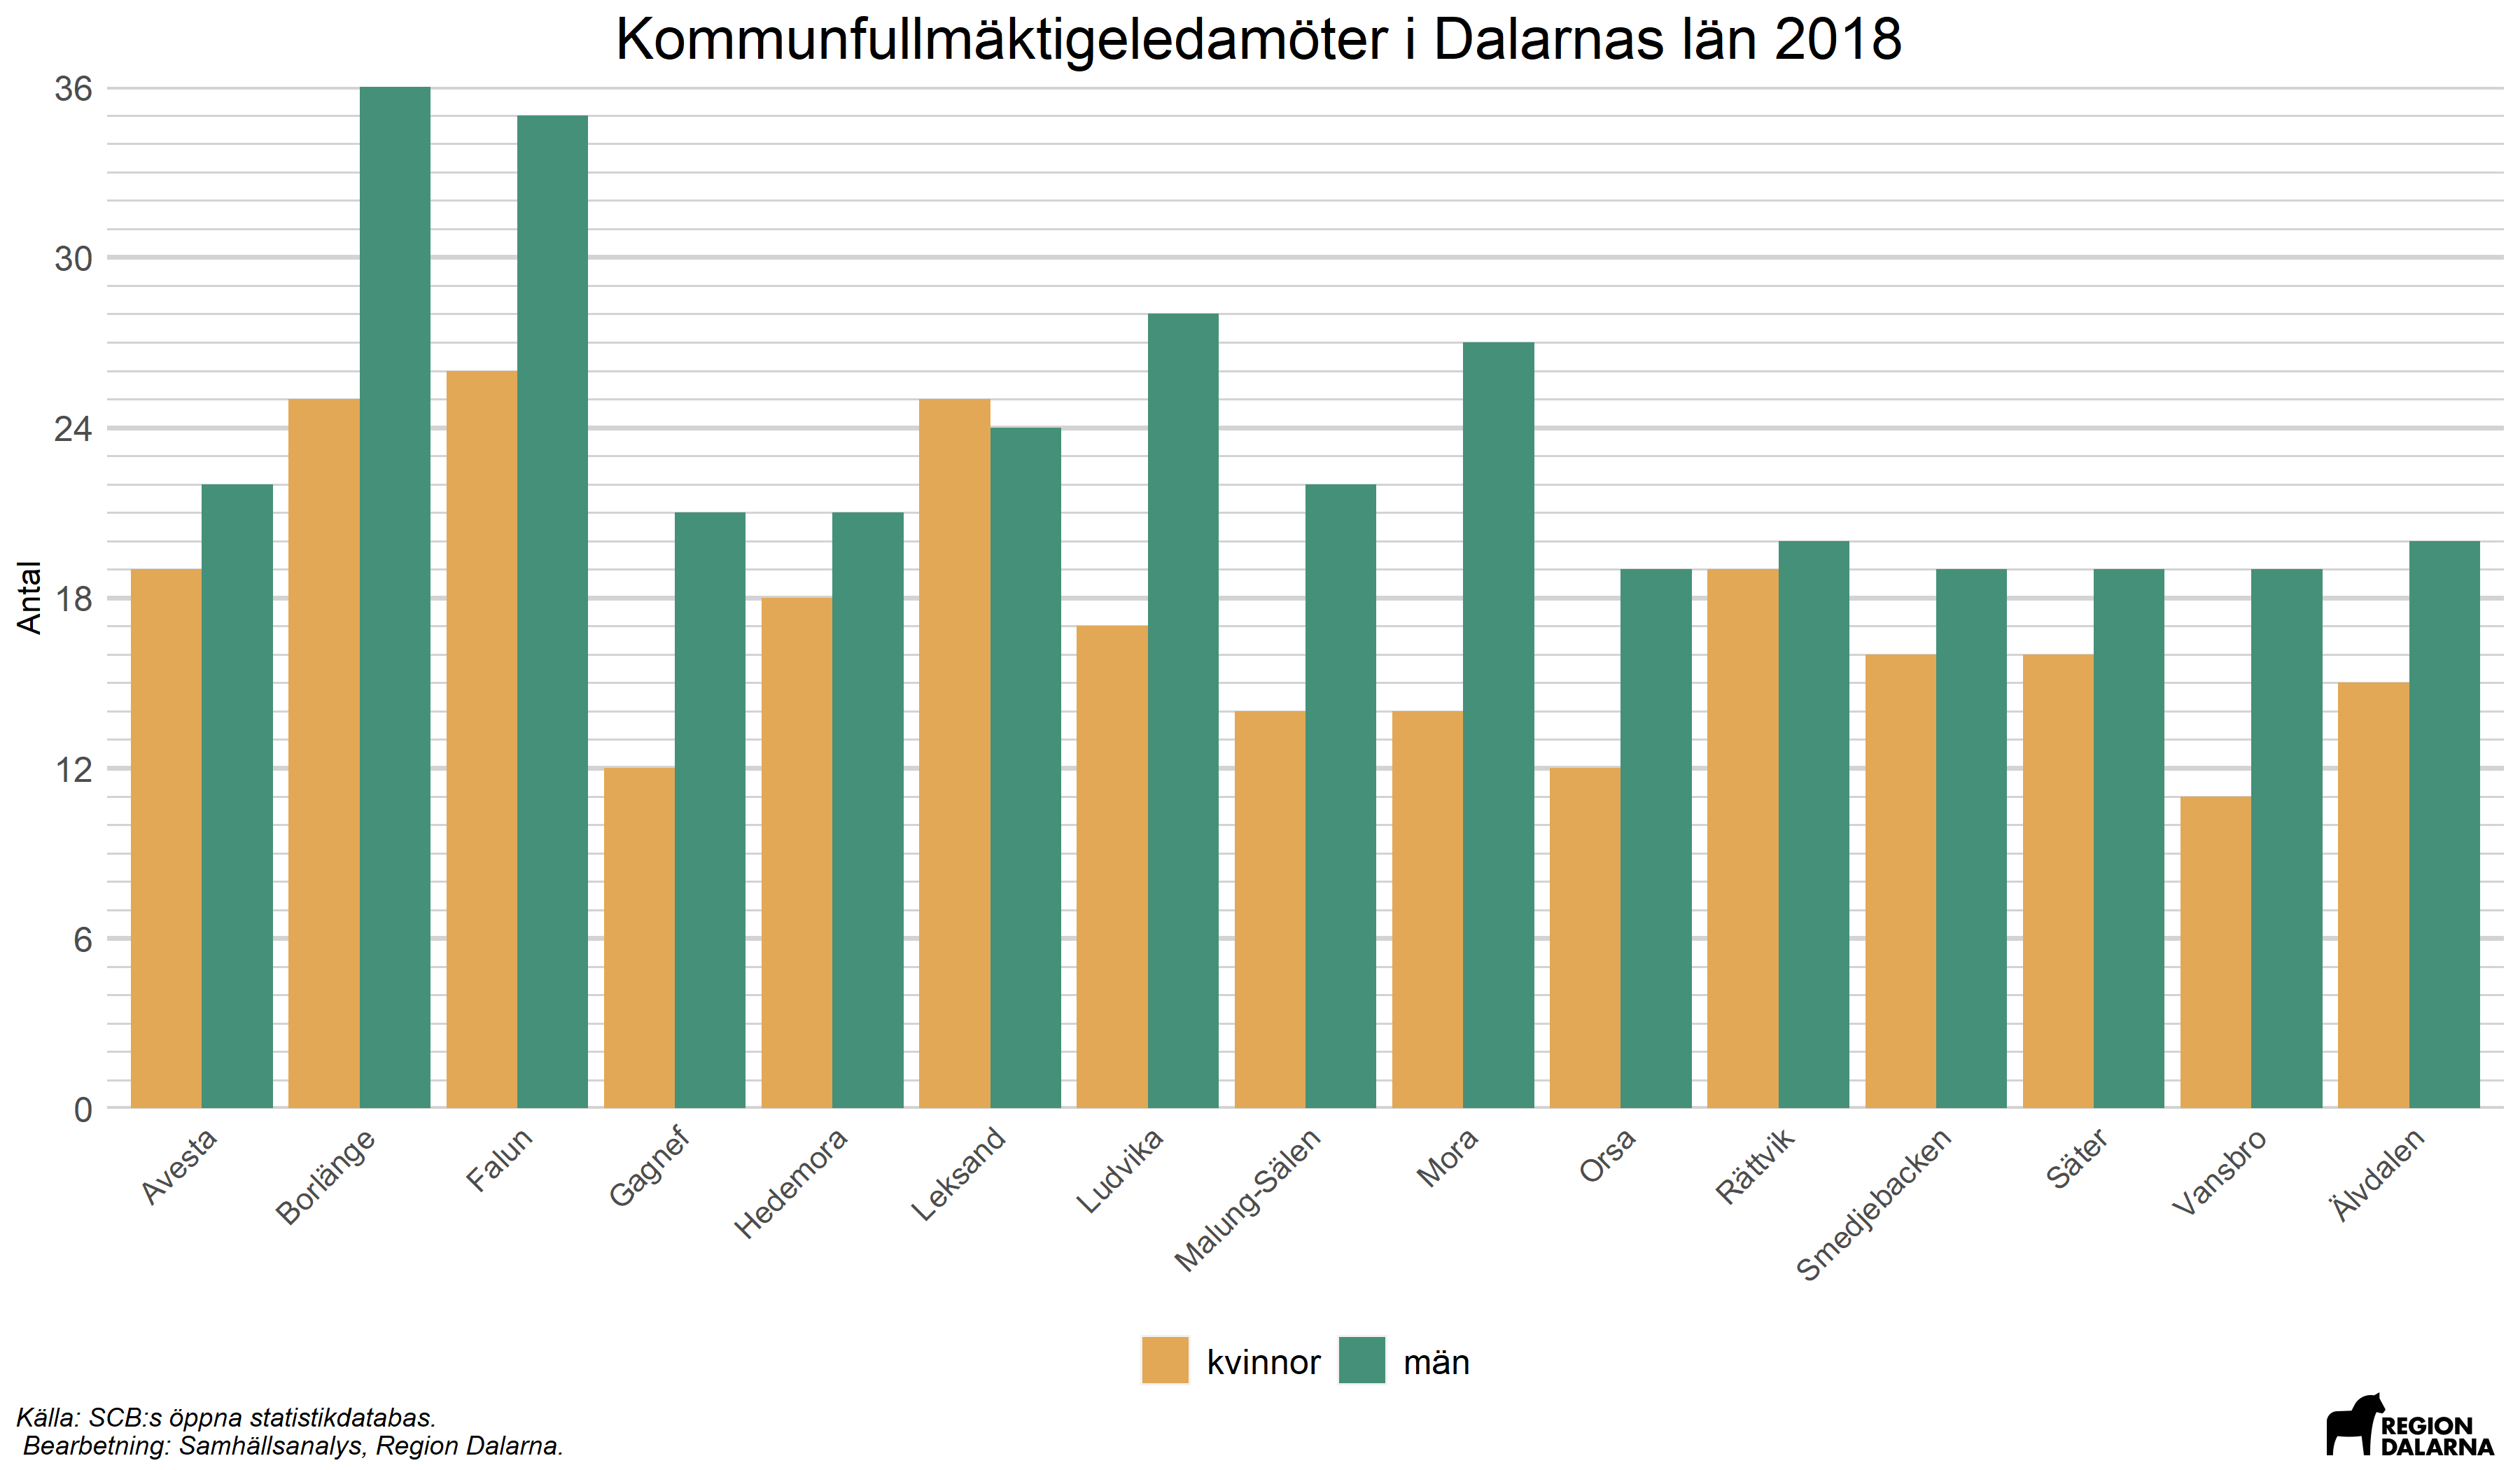
\includegraphics[width=0.9\linewidth]{G:/skript/projekt/kvinnor_man/Projekt_kvinnor_man/Diagram/kommunfullmäktige_Dalarnas län} \end{center}

\hypertarget{chefsskap}{%
\subsection{Chefsskap}\label{chefsskap}}

Ett annat mått på makt är den ställning individen har på arbetsplatsen
och i yrkeslivet. I det först diagrammet nedan visas andelen chefer för
kön per utbildningsnivå. I samtliga grupper i Dalarna är en större andel
av männen sysselsatta i någon form av chefsposition jämfört med
motsvarande grupp kvinnor. Andelen chefer är även tydligt kopplad till
utbildningsnivå där högre utbildning är associerad med en högre andel
individer i chefspositioner. Bland gruppen sysselsatta män i Dalarna med
eftergymnasial utbildning innehar drygt 11 procent någon form av
chefsställning. Bland kvinnor med eftergymnasial utbildning är
motsvarande siffra knappt 8 procent.

I det andra diagrammet ser vi utveckling över tid. Andelen kvinnor i
chefsposition i Dalarna har nästintill fördubblats under en
tjugoårsperiod. Under samma period är andelen män i chefspositioner mer
eller mindre oförändrat. Utvecklingen över tid går därmed i en mer
jämställd riktning, även om situationen på arbetsmarknaden i nuläget är
fortsatt ojämställd.

\begin{center}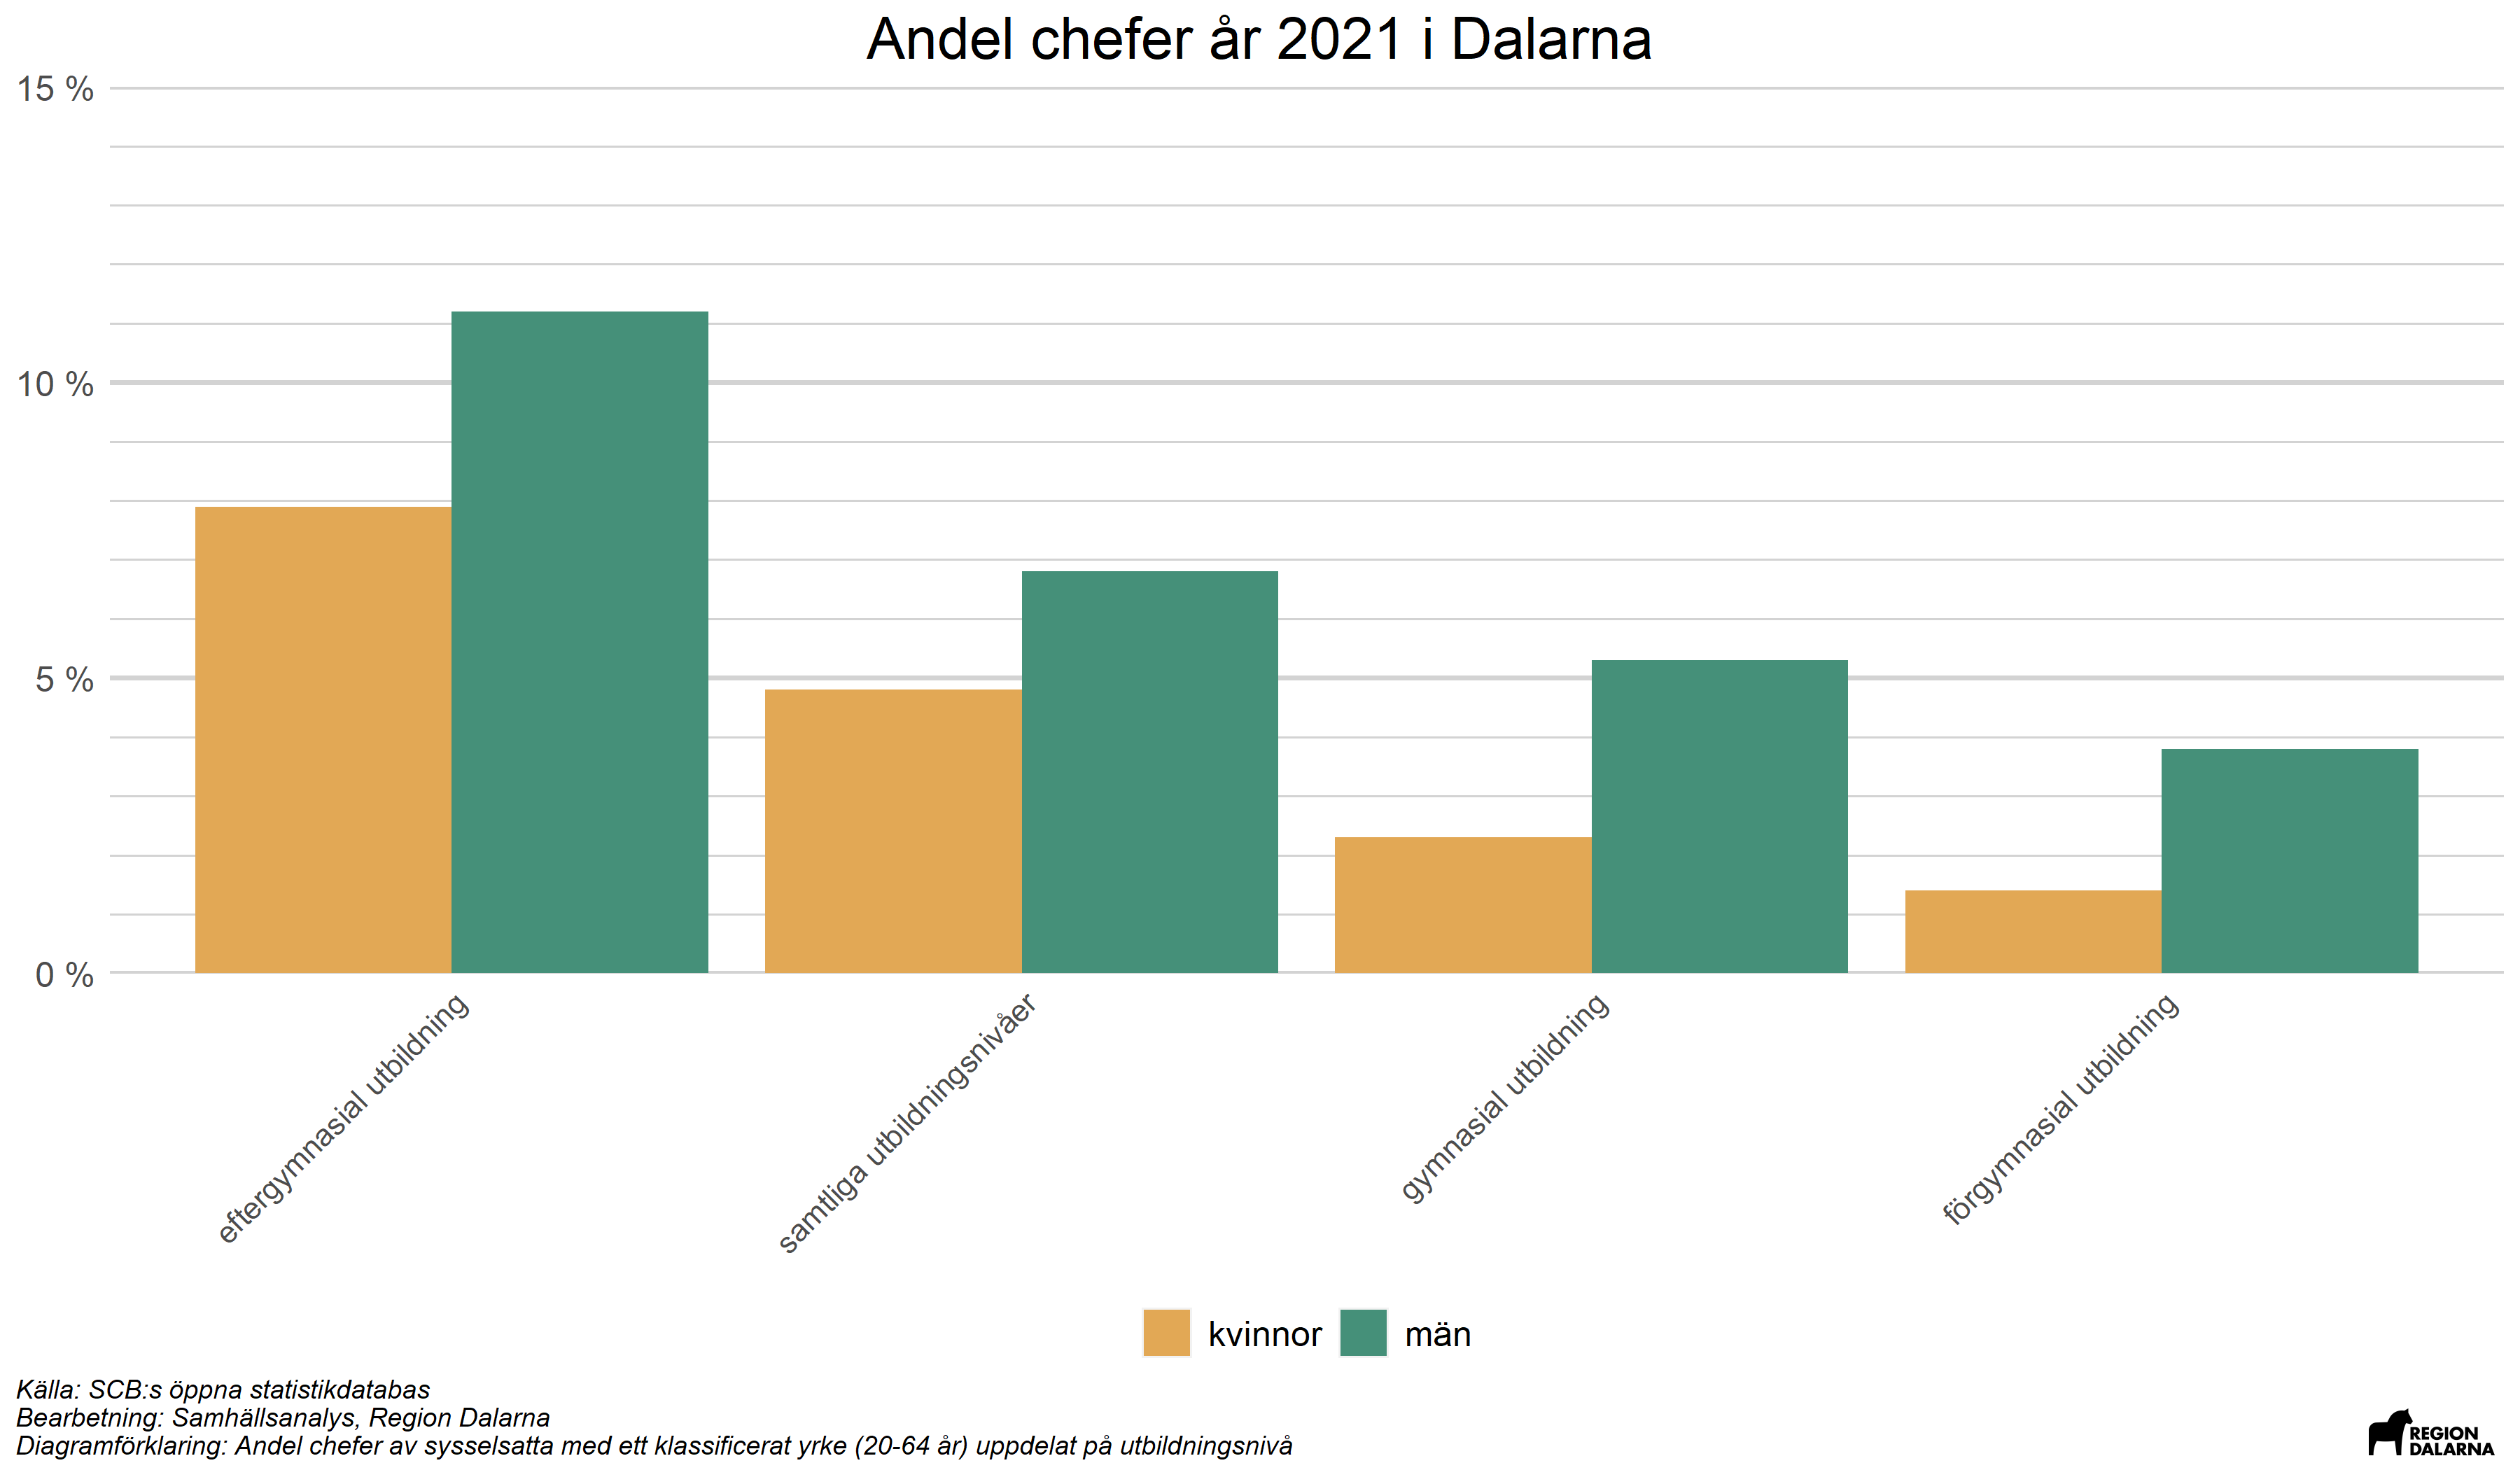
\includegraphics[width=0.9\linewidth]{G:/skript/projekt/kvinnor_man/Projekt_kvinnor_man/Diagram/andel_chefer} \end{center}

\begin{center}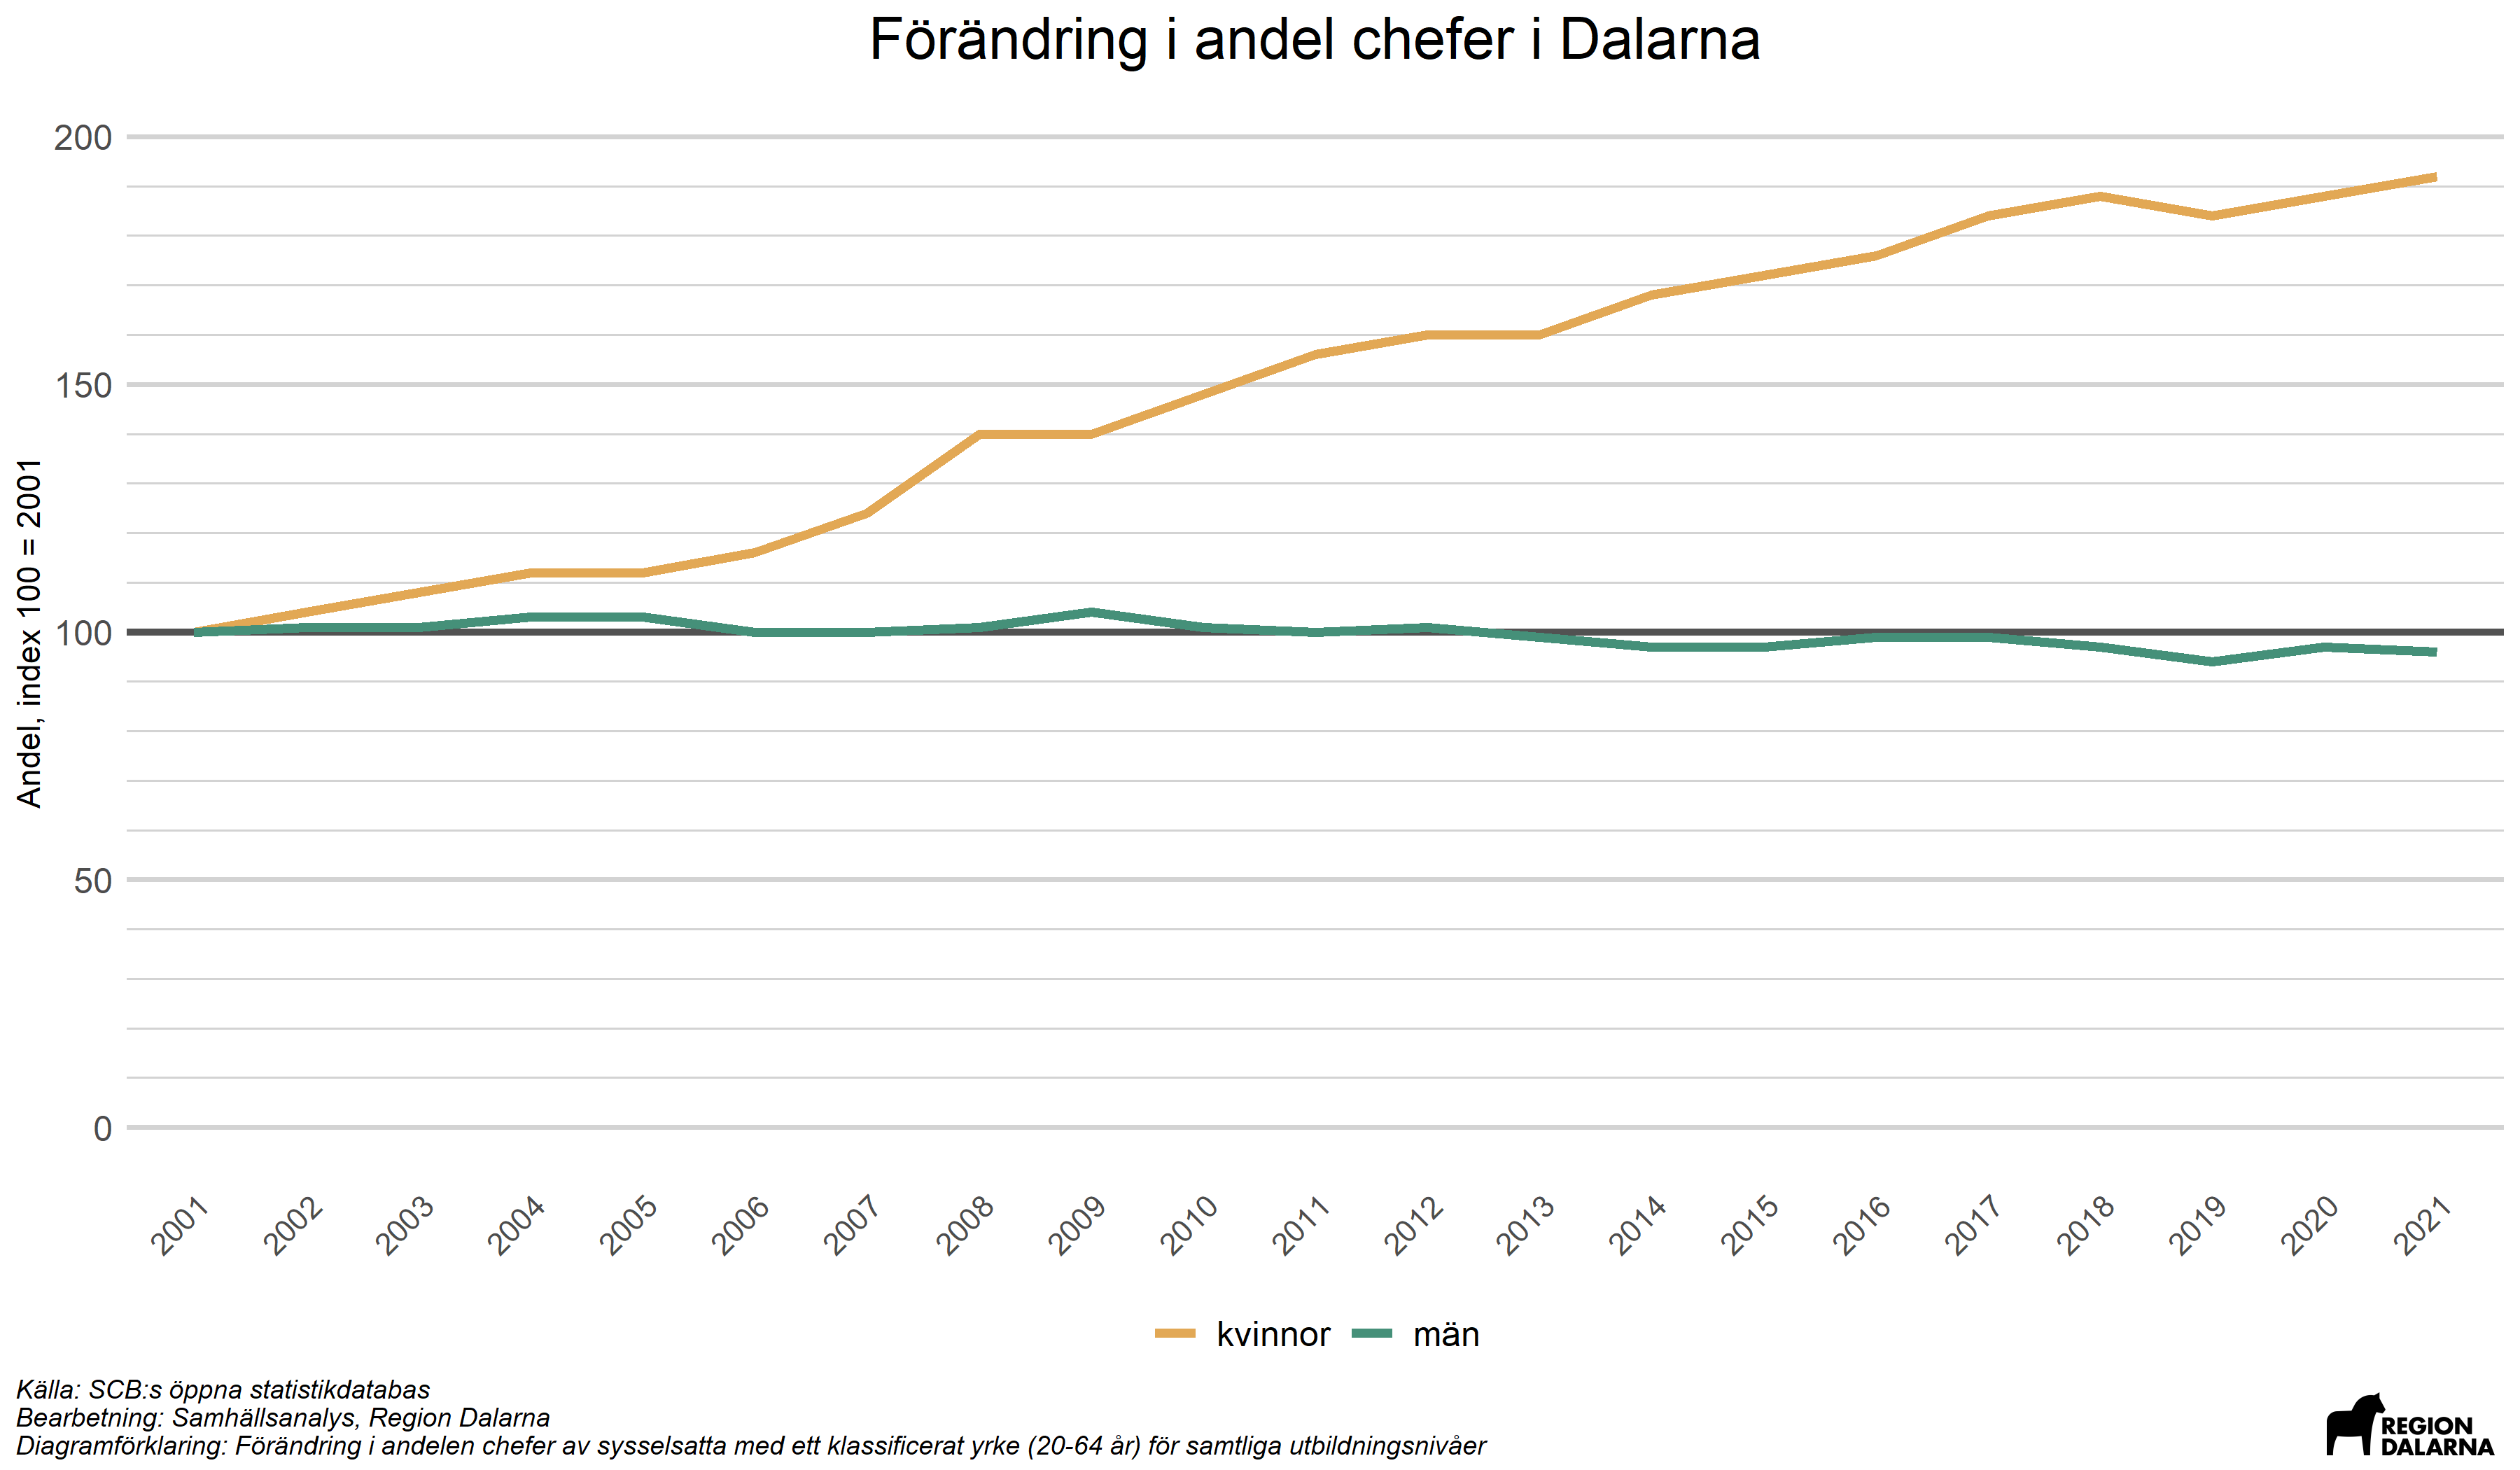
\includegraphics[width=0.9\linewidth]{G:/skript/projekt/kvinnor_man/Projekt_kvinnor_man/Diagram/andel_chefer_linje} \end{center}

\end{document}
